\documentclass[openany]{book}
\usepackage[a4paper,margin=4.72cm]{geometry}

\usepackage{graphicx}
\usepackage{siunitx} 
\usepackage{natbib}
\usepackage{mathtools}
\usepackage{amssymb}
\usepackage{amsthm}
\usepackage[italian]{babel}
\usepackage{stackengine}
\usepackage{graphicx,ifthen}
\usepackage{amsmath}
\usepackage{hyperref}
\usepackage{upgreek}
\usepackage{bm}
\usepackage{braket}
\usepackage{float}
\usepackage{cancel}
\usepackage{anyfontsize}
\usepackage{scalefnt}
\usepackage{mathtools}
\usepackage{underoverlap}
\usepackage{slashed}
\usepackage{extarrows}
\usepackage{tikz}
\usetikzlibrary{positioning}

\newtheorem{lem}{Lemma}
\newtheorem{axiom}{Assioma}
\newtheorem{defn}{Definizione}
\newtheorem{obs}{Osservazione}
\newtheorem{ex}{Esempio}
\newtheorem{notz}{Notazione}
\newtheorem{corl}{Corollario}
\newtheorem{teo}{Teorema}
\theoremstyle{remark}
\newtheorem{caso}{Caso}

\numberwithin{lem}{chapter}
\numberwithin{axiom}{chapter}
\numberwithin{teo}{chapter}
\numberwithin{defn}{chapter}
\numberwithin{obs}{chapter}
\numberwithin{ex}{chapter}
\numberwithin{equation}{chapter}

% insiemi
\newcommand{\R}{\mathbb{R}}
\newcommand{\MI}{\mathbb{I}}
\newcommand{\MO}{\mathbb{O}}
\newcommand{\N}{\mathbb{N}}
\newcommand{\C}{\mathbb{C}}
\newcommand{\HFN}{\SH_{N,F}}
\newcommand{\HBN}{\SH_{N,B}}
\newcommand{\HBFN}{\SH_{N,B/F}}
\newcommand{\SH}{\mathcal{H}}
\newcommand{\Horb}{\mathcal{H}_{orb}}
\newcommand{\Hfock}{\mathcal{H}_{Fock}}
\newcommand{\Hs}{\SH_s}

% operatori quantistici
\newcommand{\hatac}{\hat{a}_i^\dagger}
\newcommand{\hatad}{\hat{a}_i}
\newcommand{\hata}{\hat{a}}
\newcommand{\hataT}{\hat{a}^\dagger}
\newcommand{\hatb}{\hat{b}}
\newcommand{\hatbT}{\hat{b}^\dagger}
\newcommand{\hatT}{\hat{T}}
\newcommand{\hatPi}{\hat{\Pi}}
\newcommand{\hatpi}{\hat{\pi}}
\newcommand{\hatR}{\hat{R}}
\newcommand{\hatx}{\hat{x}}
\newcommand{\hatp}{\hat{p}}
\newcommand{\hatH}{\hat{H}}
\newcommand{\hath}{\hat{h}}
\newcommand{\hatfH}{\hat{\mathcal{H}}}
\newcommand{\hatS}{\hat{S}}
\newcommand{\hatO}{\hat{O}}
\newcommand{\hatL}{\hat{L}}
\newcommand{\hatU}{\hat{U}}
\newcommand{\hatQ}{\hat{Q}}
\newcommand{\hatA}{\hat{A}}
\newcommand{\hatB}{\hat{B}}
\newcommand{\hatP}{\hat{P}}
\newcommand{\hatE}{\hat{E}}
\newcommand{\hatJ}{\hat{J}}
\newcommand{\hatN}{\hat{N}}
\newcommand{\hatn}{\hat{n}}
\newcommand{\hatUT}{\hat{U}(t)}
\newcommand{\hatsz}{\hat{s}_3}
\newcommand{\hatphi}{\hat{\phi}}
\newcommand{\hatphid}{\hat{\phi}^\dagger}
\newcommand{\hatpsi}{\hat{\psi}}
\newcommand{\hatpsid}{\hat{\psi}^\dagger}
\newcommand{\hatpsib}{\hat{\bar{\psi}}}
\newcommand{\oc}{\Psi_{\sigma}^\dagger}
\newcommand{\ocq}{\Psi_{\sigma}}
\newcommand{\slp}{\slashed{p}}

% vettori
\newcommand{\vx}{\bm{x}}
\newcommand{\bx}{\bar{x}}
\newcommand{\vy}{\bm{y}}
\newcommand{\vr}{\bm{r}}
\newcommand{\vp}{\bm{p}}
\newcommand{\vq}{\bm{q}}
\newcommand{\vk}{\bm{k}}
\newcommand{\vv}{\bm{v}}
\newcommand{\vj}{\bm{j}}
\newcommand{\vJ}{\bm{J}}
\newcommand{\vK}{\bm{K}}
\newcommand{\vA}{\bm{A}}
\newcommand{\vE}{\bm{E}}
\newcommand{\vB}{\bm{B}}

% operatori matematici
\newcommand{\mybraket}[2]{\langle #1 | #2 \rangle}
\newcommand{\mybrakett}[3]{\langle #1 | #2 | #3 \rangle}
\newcommand{\vmedio}[1]{\langle #1 \rangle}
\newcommand{\comm}[2]{[#1,#2]}
\newcommand{\acomm}[2]{\{#1,#2\}}
\newcommand{\tr}[1]{\textnormal{tr}(#1)}
\newcommand{\Tr}{\textnormal{Tr}}
\newcommand{\nsum}{\sum\nolimits}
\newcommand{\intR}{\int_{\mathbb{R}}}
\newcommand{\ot}{\otimes}
\newcommand{\op}{\oplus}
\newcommand{\p}{\partial}
\newcommand{\dg}{\dagger}
\newcommand{\contr}[1]{\overbracket{#1}}

% quantità
\newcommand{\amp}{\mathcal{A}}
\newcommand{\EM}{\mathcal{M}}
\newcommand{\dL}{\mathcal{L}}
\newcommand{\ML}{\Lambda}
\newcommand{\psib}{\bar{\psi}}
\newcommand{\mm}{g_{\mu\nu}}

% stati quantistici
\newcommand{\sv}{\ket{0}}
\newcommand{\kO}{\ket{\Omega}}
\newcommand{\bO}{\bra{\Omega}}
\newcommand{\ua}{\uparrow}
\newcommand{\da}{\downarrow}
\newcommand{\vpsi}{\psi(\bm{x},t)}
\newcommand{\tvpsi}{\Tilde{\psi}(\bm{x},t)}
\newcommand{\ipsi}{\psi(x,t)}

% gruppi ed algebre
\newcommand{\g}{\mathfrak{g}}
\newcommand{\su}{\mathfrak{su}}
\newcommand{\so}{\mathfrak{so}}

% spinori e antispinori
\newcommand{\ub}{\bar{u}}
\newcommand{\vb}{\bar{v}}
\newcommand{\sdu}{u_s}
\newcommand{\sdv}{v_s}
\newcommand{\sdup}{u_{s'}}
\newcommand{\sdvp}{v_{s'}}

% spinori e antispinori hermitiani
\newcommand{\sdud}{u^\dg_s}
\newcommand{\sdvd}{v^\dg_s}
\newcommand{\sdudp}{u^\dg_{s'}}
\newcommand{\sdvdp}{v^\dg_{s'}}

% spinori e antispinori hermitiani coniugati
\newcommand{\sdub}{\bar{u}_s}
\newcommand{\sdvb}{\bar{v}_s}
\newcommand{\sdubp}{\bar{u}_{s'}}
\newcommand{\sdvbp}{\bar{v}_{s'}}

\makeindex
\title{\textbf{APPUNTI DI INTRODUZIONE ALLA TEORIA DEI CAMPI}}
\author{Manuel Gabriele Moretti}
\date{Settembre 2025}

\begin{document}

\maketitle
\pagenumbering{roman}
\tableofcontents
\newpage

\pagenumbering{arabic}
\chapter{Richiami di Relatività speciale}
La Relatività speciale si basa due principi fondamentali:
\begin{enumerate}
    \item le leggi della fisica sono invarianti in tutti i sistemi di riferimento inerziali;
    \item la luce si propaga nel vuoto a velocità costante, indipendentemente dallo stato di moto della sorgente o dell'osservatore.
\end{enumerate}
Si definisce la metrica dello spaziotempo, o di Minkowski, $g_{\mu\nu}$ come
\begin{equation}
\label{eq: metrica ST}
    g_{\mu\nu} = 
    \begin{pmatrix}
        1 & 0 & 0 & 0 \\
        0 & -1 & 0 & 0 \\
        0 & 0 & -1 & 0 \\
        0 & 0 & 0 & -1
    \end{pmatrix}
    \equiv g^{\mu\nu},
\end{equation}
per cui $g_{\mu\nu}g^{\mu\nu} = \MI$, o più in generale $g_{\mu\rho}g^{\rho\nu} = \delta^\nu_\mu$. In generale, un quadrivettore è un vettore a quattro componenti e si indica con
\begin{equation}
    a^\mu = (a^0,a^1,a^2,a^3) = (a^0,a^i) = (a^0,\bm{a}),
\end{equation}
dove $\bm{a}$ è il classico trivettore. Data la metrica in \eqref{eq: metrica ST}, il prodotto scalare tra due quadrivettori $a^\mu$ e $b^\mu$ è definito come
\begin{equation}
\label{eq: defn. prodotto scalare QV}
    a_\mu b^\mu = a_0b^0 - a_ib^i = a_0b^0 - \bm{a}\cdot\bm{b}.
\end{equation}
Il modulo quadro di un quadrivettore $a^\mu$ quindi è definito come
\begin{equation}
\label{eq: defn. modulo quadro QV}
    a_\mu a^\mu = a_0^2-|\bm{a}|^2 = (a^\mu)^2.
\end{equation}
L'elemento invariante in Relatività speciale è la distanza spaziotemporale
\begin{equation}
\label{eq: defn. s^2}
    s^2 = c^2t^2 - x_ix^i,
\end{equation}
infatti rispetto a trasformazioni del tipo $(t,x^i)\to(t',x'^i)$ si ha
\begin{equation}
\label{eq: invarianza s^2 per TdL}
    s^2 = c^2t^2 - x_ix^i = c^2t'^2 - x_i'x'^i.
\end{equation}
Il set di trasformazioni lineari che legano $(t,x^i)$ a $(t',x'^i)$ è detto gruppo di Lorentz, quindi si dice che la distanza $s^2$ è invariante rispetto a trasformazioni di Lorentz, che a loro volta vengono dette isometrie. La trasformazione di Lorentz di $x^\mu$ è data da
\begin{equation}
\label{eq: TdL di x^mu}
    x'^\mu = \Lambda^\mu_\nu x^\nu = \Lambda^\mu_0 x^0 + \Lambda^\mu_i x^i,
\end{equation}
dove le $\Lambda^\mu_\nu$ sono le matrici di Lorentz. Tramite la definizione \eqref{eq: defn. modulo quadro QV} si può scrivere la relazione \eqref{eq: invarianza s^2 per TdL} come
\begin{equation}
    s^2 = x^\mu x_\mu = x'^\mu x'_\mu,
\end{equation}
che equivale alla condizione
\begin{equation}
    g_{\mu\nu}x^\mu x^\nu = g_{\mu\nu}x'^\mu x'^\nu,
\end{equation}
che, usando la \eqref{eq: TdL di x^mu} e arrangiandola opportunamente, diventa
\begin{equation}
    g_{\mu\nu}x^\mu x^\nu = g_{\mu\nu}\Lambda^\mu_\rho \Lambda^\nu_\sigma x^\rho x^\sigma,
\end{equation}
la quale è verificata se e solo se
\begin{equation}
\label{eq: principio di RS}
    g_{\mu\nu}\Lambda^\mu_\rho \Lambda^\nu_\sigma = g_{\rho\sigma}.
\end{equation}
L'equazione \eqref{eq: principio di RS} viene spesso indicata con il nome di principio di relatività speciale, in quanto è la relazione che assicura che l'intervallo tra due punti dello spaziotempo $(x^\mu,x'^\mu)$ in un sistema di riferimento inerziale e $(\bx^\mu,\bx'^\mu)$ in un altro sistema di riferimento inerziale sia invariante. Questo fatto si può dimostrare nel seguente modo. Si considerano i due invarianti
\begin{equation}
    (x-x')^2 = (x-x')^\mu(x-x')_\mu,\quad(\bx-\bx')^2 = (\bx-\bx')^\mu(\bx-\bx')_\mu
\end{equation}
e usando la \eqref{eq: TdL di x^mu} si riscrive il secondo in modo da ottenere la relazione
\begin{equation}
    \begin{split}
        (\bx-\bx')^\mu(\bx-\bx')_\mu &= \Lambda_\nu^\mu(x-x')^\nu g_{\mu\sigma}(\bx-\bx')^\sigma \\
        &= g_{\mu\sigma}\Lambda_\nu^\mu(x-x')^\nu\Lambda^\sigma_\rho(x-x')^\rho \\
        &= g_{\mu\sigma}\Lambda_\nu^\mu\Lambda^\sigma_\rho(x-x')^\nu(x-x')^\rho,
    \end{split}
\end{equation}
la quale è verificata solo se $g_{\mu\sigma}\Lambda_\nu^\mu\Lambda^\sigma_\rho=g_{\nu\rho}$, condizione che coincide proprio con il principio di Relatività speciale. Usando appunto la \eqref{eq: principio di RS} si ha che
\begin{equation}
    \begin{split}
        (\bx-\bx')^\mu(\bx-\bx')_\mu &= g_{\mu\sigma}\Lambda_\nu^\mu\Lambda^\sigma_\rho(x-x')^\nu(x-x')^\rho \\
        &= g_{\nu\rho}(x-x')^\nu(x-x')^\rho \\
        &= (x-x')_\rho(x-x')^\rho,
    \end{split}
\end{equation}
verificando quindi l'invarianza di $s^2$ per trasformazioni di Lorentz. Per la precisione, il gruppo di Lorentz è contenuto nel gruppo di Poincaré che comprende trasformazioni più generali, la trasformazione di Poincaré di $x^\mu$ è infatti data da
\begin{equation}
\label{eq: TdP di x^mu}
    x'^\mu  =\Lambda^\mu_\nu x^\nu + a^\mu.
\end{equation}
Tuttavia, nella dimostrazione appena svolta l'ulteriore quadrivettore $a^\mu$ che compare in \eqref{eq: TdP di x^mu} non ha alcun effetto dato che si sono considerati intervalli, i quali appunto non sono sensibili alle semplici traslazioni nello spaziotempo. 
\begin{notz}
    D'ora in avanti, salvo eccezioni, si userà la scala di unità naturale che consiste nel porre $\hbar = 1$ e $c = 1$.
\end{notz}
Si definiscono infine gli operatori di derivazione covariante e controvariante rispettivamente come
\begin{equation}
    \p_\mu \equiv \frac{\p}{\p x^\mu} = \bigg(\frac{\p}{\p t},\nabla\bigg),\quad \p^\mu \equiv \frac{\p}{\p x_\mu} = \bigg(\frac{\p}{\p t},-\nabla\bigg).
\end{equation}
Appare subito evidente che $\p^\mu x^\nu = g^{\mu\nu}$, che $\p_\mu x^\mu = \MI$ e che $\p_\mu x^\nu = g_\mu^\nu$. Inoltre, $\p^\mu$ trasforma esattamente come $x^\mu$, per cui
\begin{equation}
\label{eq: TdL di d^mu}
    \bar{\p}^\mu = \Lambda^\mu_\nu\p^\nu.
\end{equation}
Infatti, da
\begin{equation}
    \bar{\p}^\rho\bx^\sigma = (\Lambda^\rho_\mu\p^\mu)(\Lambda^\sigma_\nu x^\nu + a^\sigma) = \Lambda^\rho_\mu\Lambda^\sigma_\nu\p^\mu x^\nu = \Lambda^\rho_\mu\Lambda^\sigma_\nu g^{\mu\nu} = g^{\rho\sigma}
\end{equation}
che, per il principio di Relatività speciale \eqref{eq: principio di RS}, coincide proprio con $\p^\mu x^\nu = g^{\mu\nu}$, per cui
\begin{equation}
    \bar{\p}^\rho\bx^\sigma = \p^\rho x^\sigma.
\end{equation}
Inoltre, si può dimostrare che anche $\p^2 = \p^\mu\p_\mu \equiv\square$ è invariante per trasformazioni di Lorentz. Infatti, si può scrivere $\p^2$ come
\begin{equation}
    \p^\mu\p_\mu = g_{\mu\nu}\p^\mu\p^\nu,
\end{equation}
mentre $\bar{\p}^2 = \bar{\p}^\mu\bar{\p}_\mu \equiv \bar{\square}$ può essere riscritto come
\begin{equation}
    \bar{\p}^\mu\bar{\p}_\mu = g_{\mu\nu}\Lambda^\mu_\rho\Lambda^\nu_\sigma\p^\rho\p^\sigma = g_{\rho\sigma}\p^\rho\p^\sigma = \p^\rho\p_\rho,
\end{equation}
dove si è sempre usata la \eqref{eq: principio di RS}. Dunque, si ha che il l'operatore d'Alembert è invariante per trasformazioni di Lorentz, ovvero
\begin{equation}
\label{eq: invarianza per TdL di OD'AL}
    \square = \bar{\square}.
\end{equation}


\chapter{Equazione di Klein-Gordon}
L'obiettivo è quello di trovare un'equazione del moto quantistica che sia in accordo con la teoria della Relatività. Già Schr\"odinger aveva tentato questa impresa, ma abbandonò l'idea a causa di alcune conseguenze problematiche che l'eventuale soluzione implicava. Non considerando le questioni relativistiche, arrivò alla formulazione dell'equazione di Schr\"odinger, la quale funziona perfettamente ma non è in accordo con la Relatività, in primis il tempo non viene considerato come una coordinata ma come un semplice parametro.

In Meccanica quantistica non relativistica ogni stato è definito da un vettore $\ket{\psi}$ appartenente ad uno spazio di Hilbert $\SH$ e ogni misura di un'osservabile $O$ restituisce come risultato l'autovalore del corrispondente operatore hermitiano $\hatO$. L'evoluzione temporale di un sistema quantistico è codificato nell'equazione di Schr\"odinger, informazione che può poi essere convenientemente racchiusa in un operatore hermitiano di evoluzione temporale $\hatU$ definito a posteriori. L'equazione di Schr\"odinger nella sua forma più generale è
\begin{equation}
\label{eq: eq. schro. forma generale generale}
    i\hbar\frac{\p}{\p t}\ket{\psi} = \hatH\ket{\psi},\quad\ket{\psi}\in\SH.
\end{equation}
Considerando una particella libera, se si proietta l'equazione \eqref{eq: eq. schro. forma generale generale} sullo spazio delle coordinate considerando il prodotto scalare con $\bra{\vx}$, si associa all'osservabile $p$ l'operatore hermitiano $\hatp=-i\hbar\nabla$ e si ricorda che l'hamiltoniana di una particella libera è 
\begin{equation}
\label{eq: hamiltoniana particella libera}
    \hatH = \frac{\hatp^2}{2m},
\end{equation}
allora si ottiene l'equazione di Schr\"odinger per la particella libera
\begin{equation}
\label{eq: eq. schro. particella libera}
    i\hbar\frac{\p\vpsi}{\p t} = -\frac{\hbar^2}{2m}\nabla^2\vpsi,\quad\vpsi = \mybraket{\vx}{\psi}.
\end{equation}
Le funzioni d'onda soluzioni dell'equazione \eqref{eq: eq. schro. particella libera} sono onde piane della forma $\ipsi=Ne^{-i(\omega t-\vk\cdot\vx)}$. Per rendere relativistica l'equazione \eqref{eq: eq. schro. particella libera} si potrebbe pensare di sostituire la relazione di dispersione della particella libera relativistica
\begin{equation}
\label{eq: eq. mass-shell}
    E^2=p^2c^2+m^2c^4.
\end{equation}
Quindi, considerando la radice di \eqref{eq: eq. mass-shell} si può pensare di porre
\begin{equation}
\label{eq: hamiltoniana KG}
    \hatH\equiv (E^2)^{1/2} = \sqrt{p^2c^2+m^2c^4}.
\end{equation}
In linea di principio, il secondo membro di \eqref{eq: hamiltoniana KG} può essere sia positivo che negativo, nulla a priori permette di eliminare uno dei due casi. Sorgono quindi due problemi: il primo è che prendendo la radice della relazione di dispersione di ottengono energie negative; il secondo è che la radice quadrata di un operatore differenziale non è un'operazione matematicamente ben definita. Per il momento, il discorso sulle energie negative viene lasciato da parte e si considerano solo quelle positive di \eqref{eq: hamiltoniana KG}, mentre per aggirare il secondo problema si può pensare di sviluppare in serie l'hamiltoniana in \eqref{eq: hamiltoniana KG}, per cui si ha
\begin{equation}
\label{eq: sviluppo in serie hamiltoniana KG}
    \hatH = \sqrt{p^2c^2+m^2c^4} = mc^2 + mc^2\frac{p^2}{2m^2c^2} + \cdots = mc^2 + \frac{p^2}{2m} + \cdots.
\end{equation}
In questo modo, almeno al primo ordine, l'hamiltoniana \eqref{eq: sviluppo in serie hamiltoniana KG} corrisponde all'hamiltoniana di particella libera \eqref{eq: hamiltoniana particella libera}, somma dell'energia a riposo e del termine cinetico della Meccanica quantistica. Si può ora pensare di scrivere una nuova equazione di Schr\"odinger di forma
\begin{equation}
\label{eq: eq. pre-KG}
    i\hbar\frac{\p\vpsi}{\p t} = (\sqrt{\hbar^2c^2\nabla^2 + m^2c^4})\vpsi.
\end{equation}
Tuttavia, l'equazione \eqref{eq: eq. pre-KG} presenta un grande problema che coinvolge proprio lo sviluppo in serie dell'hamiltoniana. Definendo $\hatH$ in quel modo si ottiene un operatore che corrisponde ad una serie infinita di derivate di ordini sempre crescenti, ma così facendo l'operatore che ne risulta non è più locale, ovvero al posto che restituire una variazione infinitesima, ne restituisce una finita. In ogni caso comunque non si è risolto il problema delle energie negative, per ora solo accantonato, ma anche se si provasse a considerarle si avrebbe a che fare con un sistema ``unbounded from below'', ossia non limitato inferiormente. L'energia infatti se si permette che possa essere negativa, può allora assumere qualsiasi valore senza un limite inferiore che permetta di avere uno stato fondamentale del sistema. 

Osservando l'equazione \eqref{eq: eq. pre-KG} si nota uno ``sbilanciamento'' nell'ordine delle derivate spaziali e temporali, ispirandosi all'equazione di d'Alembert, si può pensare di usare come hamiltoniana direttamente $E^2$ senza prederne la radice, così facendo si ricava l'equazione di Klein-Gordon
\begin{equation}
\label{eq: eq. Klein-Gordon}
    -\hbar^2\frac{\p^2\ipsi}{\p t^2}=(-\hbar^2c^2\nabla^2+m^2c^4)\ipsi.
\end{equation}
In unità naturali, l'equazione \eqref{eq: eq. Klein-Gordon}, arrangiandola opportunamente, diventa
\begin{equation}
\label{eq: eq. Klein-Gordon U.N.}
    (\square+m^2)\vpsi=0,
\end{equation}
le cui soluzioni sono\footnote{In unità naturali, $E=\omega$ e $\vp=\vk$.}
\begin{equation}
    \psi(x^\mu)=Ne^{-i(Et-\vp\cdot\vx)}=Ne^{-ip^\mu x_\mu},\quad E=\pm\sqrt{p^2+m^2}.
\end{equation}
L'equazione \eqref{eq: eq. Klein-Gordon U.N.} è in accordo con la Relatività speciale, infatti se si opera una trasformazione $(\square,\psi(x^\mu))\to(\bar{\square},\bar{\psi(}\bx^\mu))$ l'equazione mantiene la medesima forma dato che 
\begin{equation}
    \psi(x^\mu) = \bar{\psi(}\bx^\mu),\quad \square = \bar{\square}.
\end{equation}
Infatti, il primo principio della Relatività speciale richiede che ogni fenomeno fisico sia lo stesso in ogni sistema di riferimento inerziali, ovvero che due osservatori $A$ e $B$ in due sistemi di riferimento inerziali diversi ottengono gli stessi risultati per ogni possibile esperimento, oltre ad essere d'accordo sulle predizioni dei risultati i tali esperimenti. Quindi, se $A$ afferma che un sistema che si trova nel punto $x^\mu$ del suo sistema di riferimento inerziale è descritto dalla funzione d'onda $\psi(x^\mu)$ e $B$ afferma che lo stesso sistema, che si trova nel punto $\bx^\mu$ del suo sistema di riferimento è descritto dalla funzione d'onda $\bar{\psi}(\bx)$, allora necessariamente deve essere 
\begin{equation}
    \psi(x^\mu) = \bar{\psi}(\bx^\mu).
\end{equation}
L'invarianza del D'Alembertiano per trasformazioni di Lorentz invece si era verificata in \eqref{eq: invarianza per TdL di OD'AL}. Tuttavia, l'equazione \eqref{eq: eq. Klein-Gordon U.N.}, per quanto elegante, presenta un grave problema: la densità di probabilità non è definita positiva. Questo è il motivo per cui Schr\"odinger abbandonò l'equazione dopo averla derivata, in quanto tutta l'interpretazione probabilistica della Meccanica quantistica viene invalidata se non è possibile definire una densità di probabilità. Per verificarlo si considerano l'equazione \eqref{eq: eq. Klein-Gordon U.N.} e la sua coniugata, moltiplicate rispettivamente per $\vpsi^*$ e $\vpsi$, 
\begin{equation}
    \begin{cases}
        \vpsi^*(\square+m^2)\vpsi=0 \\
        \vpsi(\square+m^2)\vpsi^*=0
    \end{cases},
\end{equation}
calcolando la differenza tra la prima e la seconda equazione si trova
\begin{equation}
    \begin{split}
        \psi^*\square\psi + \vpsi^*m^2\psi - \psi\square\psi^* - \psi m^2\psi^* &= 0 \\
        \psi^*\square\psi - \psi\square\psi^* &= 0 \\
        \p^\mu(\psi^*\p_\mu\psi - \psi\p_\mu\psi^*) &= 0 \\
        \frac{\p}{\p t}\bigg(\psi^*\frac{\p}{\p t}\psi - \psi\frac{\p}{\p t}\psi^*\bigg) - \nabla\bigg(\psi^*\nabla\psi - \psi\nabla\psi^*\bigg) &= 0, \\
    \end{split}
\end{equation}
che apparentemente sembra avere la forma di un'equazione di continuità, tuttavia, anche se il termine $\psi^*\nabla\psi - \psi\nabla\psi^*$ ha effettivamente la forma di una corrente di probabilità $\vj$, il termine 
\begin{equation}
    \psi^*\frac{\p}{\p t}\psi - \psi\frac{\p}{\p t}\psi^*
\end{equation}
non può essere interpretato come una densità di probabilità dato che la differenza non è obbligatoriamente positiva. Pertanto, dall'equazione \eqref{eq: eq. Klein-Gordon U.N.} non è possibile derivare un'equazione di continuità dato che la densità di probabilità $\rho$ non è definita positiva, impedendo la definizione di una quadricorrente di probabilità $j^\mu = (j^0,j^i) = (\rho,\vj)$.

\include{Capitolo 3 - Richiami di TdG }
\chapter{Campi locali}
In Meccanica classica che descrive il punto materiale, un sistema è descritto da un set di coordinate generalizzate $\{q_i\}$ e dalla lagrangiana $L(q_i,\dot{q}_i)$ che dipende dalle $q_i$ e dalle rispettive velocità generalizzate $\dot{q}_i$. Dal principio di minima azione $\delta S = 0$, dove $S = \int_{t}L(q_i,\dot{q}_i)\,dt$ è l'azione, si possono derivare le equazioni del moto di Eulero-Lagrange. In una teoria di campo ruolo delle coordinate $q_i$ è assunto proprio dal campo $\phi(\vx,t)$ in cui l'indice $i$ delle $q_i$ viene rimpiazzato da $\vx$ che varia con continuità. Come già accennato, la posizione non è un operatore come in Meccanica quantistica ma un parametro al pari del tempo $t$, entrambi aventi il ruolo di ``etichettare'' il campo $\phi(\vx,t)$ che si estende su un numero infinito di valori delle coordinate. Tuttavia, in una teoria di campo si prevede che possano coesistere campi diversi in uno stesso punto dello spazio, per cui si usa un indice aggiuntivo $\phi_i(\vx,t)$ per distinguerli. I campi vengono poi associati ad una lagrangiana che ne determina l'evoluzione temporale. Le teorie di campo che si trattano sono teorie locali, in cui la dinamica del sistema non collega punti diversi dello spazio istantaneamente, rispettando quindi il principio della Relatività speciale e la causalità degli eventi. Nelle teorie locali, i campi in qualsiasi regione dello spazio $R$ comunicano con lo spazio esterno ad $R$ solo attraverso i loro comportamento sulla superficie $\sigma$ di $R$. 
\begin{figure}[h]
    \centering
    \begin{tikzpicture}[scale=0.7]
        % Assi
        \draw[->] (0,0) -- (8,0) node[right] {$t$};
        \draw[->] (0,0) -- (0,4) node[above] {$x$};
        % Livelli x1 e x2
        \draw[dashed] (0,1) -- (2,1);
        \draw[dashed] (0,3) -- (2,3);
        \node[left] at (0,1) {$x_1$};
        \node[left] at (0,3) {$x_2$};
        % Tempi t1 e t2
        \draw[dashed] (2,0) -- (2,1);
        \draw[dashed] (7,0) -- (7,1);
        \node[below] at (2,0) {$t_1$};
        \node[below] at (7,0) {$t_2$};
        % Rettangolo R
        \draw (2,1) rectangle (7,3);
        \node at (4.5,2) {$R$};
        % Etichette P2
        \node[left] at (2,3.3) {$P_2$};
        \node[left] at (2,1.3) {$P_1$};
        % Etichetta theta
        \node[above] at (7,3) {$\sigma$};
    \end{tikzpicture}
    \caption{evoluzione temporale del sistema da $t_1$ a $t_2$.}
    \label{fig: evoluzione temporale}
\end{figure}
Quindi, in riferimento alla figura \ref{fig: evoluzione temporale}, per specificare i campi in ogni punto dello spaziotempo all'interno di $R$ è sufficiente specificare il valore dei campi in ogni punto interno ad $R$ negli istanti $t_1$ e $t_2$, e il valore dei campi in ogni punto sulla superficie $\sigma$ in tutti gli istanti di tempo $t$ compresi tra $t_1$ e $t_1$. Date queste condizioni, la lagrangiana ed il principio di minima azione descrivono l'evoluzione temporale dei campi per ogni istante $t_1 < t < t_2$ all'interno di $R$ tramite le equazioni del moto. 

\section{Dalla prima alla seconda quantizzazione}
Il processo di trattare le coordinate $q_i$ e $p_i$ in meccanica lagrangiana ed hamiltoniana è chiamata ``prima quantizzazione'', tuttavia nelle teorie di campo si studiano oggetti che hanno un numero infinito di gradi di libertà. La transizione tra Meccanica quantistica e Teoria dei campi avviene proprio passando dai tre gradi di libertà delle coordinate $x^i$ agli infiniti descritti dai campi $\phi(x^i)$ ed applicando direttamente ad essi i criteri di quantizzazione. 
\begin{figure}[h]
    \centering
    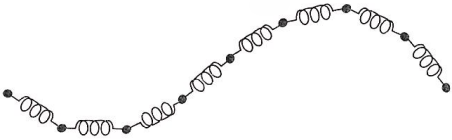
\includegraphics[width=0.5\linewidth]{Immagini/oscillatori armonici.png}
    \caption{sistema di infinite masse collegate da altrettante molle.}
    \label{fig: oscillatori armonici}
\end{figure}

Prima di effettuare questa transizione si può discutere come si descrivono in Meccanica classica sistemi con un numero infinito di gradi di libertà. A tal proposito, si consideri un numero $N$ masse collegate tra di loro da molle di costante elastica $k$, come mostrato in figura \ref{fig: oscillatori armonici}. La lagrangiana di questo sistema contiene due termini, l'energia potenziale di ogni molla e l'energia cinetica di ogni massa. Per cui, la lagrangiana è
\begin{equation}
    L = \sum_{i = 1}^{N}\frac{1}{2}\bigg[m_i\dot{x}_i^2 - k(x_i - x_{i+1})^2\bigg].
\end{equation}
Ora si supponga che si abbia un numero infinito di masse, $N\to\infty$, separate da una distanza $\epsilon$, per cui 
\begin{equation}
    L = \sum_{i = 1}^{N}\frac{\epsilon}{2}\bigg[\frac{m_i}{\epsilon}\dot{x}_i^2 - \frac{k}{\epsilon}(x_i - x_{i+1})^2\bigg],
\end{equation}
nel limite $\epsilon\to0$, la lagrangiana diventa
\begin{equation}
    L = \int\frac{1}{2}\bigg[\mu\dot{\phi}(x)^2 - Y\bigg(\frac{\p\phi(x)}{\p x}\bigg)^2\bigg]\,dx,
\end{equation}
dove $\mu = m/\epsilon$ è la densità di massa lineare, $Y = k\epsilon$ è il modulo di Young e dove si sono operate le estensioni al continuo
\begin{equation}
    \epsilon \to dx,\quad x_i \to \phi(x,t),
\end{equation}
indicando con $\phi(x,t)$ lo spostamento della singola particella localizzata nella posizione $x$ all'istante $t$. Usando le equazioni di Eulero-Lagrange per trovare le equazioni del moto si ritrova l'equazione delle onde unidimensionale 
\begin{equation}
    \frac{\p^2\phi}{\p x^2} - \frac{\mu}{Y}\frac{\p^2\phi}{\p t^2} = 0
\end{equation}
di un sistema che viaggia alla velocità $v = \sqrt{Y/\mu}$. Con questo, da una parte si è dimostrato il fatto che le onde possono propagarsi lungo una molla infinita, mentre dall'altra si è effettuata una transizione ad un sistema con infiniti gradi di libertà tutt'altro che banale. Questa generalizzazione si può vedere come il passaggio dalla lagrangiana $L(q_i,\dot{q}_i)$ ad una lagrangiana funzione dei campi e delle sue derivate spaziotemporali
\begin{equation}
    L(\phi(x^\mu),\p_\mu\phi(x^\mu)),
\end{equation}
definendo quindi l'azione $S$ come l'integrale in quattro dimensioni di una densità di lagrangiana $\mathcal{L}$
\begin{equation}
\label{eq: azione}
    S = \int\mathcal{L}\,d^4x = \int L\,dt,\quad L = \int\mathcal{L}(\phi,\p_\mu\phi)\,d^3x.
\end{equation}

\section{Trasformazioni di Poincarè}
Si consideri una funzione $f$ dipendente dalle coordinate spaziotemporali di un punto $P$. In un certo sistema di riferimento il punto $P$ ha coordinate $x^\mu$ e la funzione ha la forma $f(x^\mu)$, mentre in un altro ha coordinate $x'^\mu$, per cui la funzione è $f'(x'^\mu)$. Per un trasformazione infinitesima $x'^\mu = x^\mu + \delta x^\mu$, la variazione totale su $f$ è
\begin{equation}
    \begin{split}
        \Delta f &= f'(x'^\mu) - f(x^\mu) = f'(x^\mu + \delta x^\mu) - f(x^\mu) \\
        &= f'(x^\mu) - f(x^\mu) +\p_\mu f'(x^\mu)\delta x^\mu + O[(\delta x^\mu)^2].
    \end{split} 
\end{equation}
All'ordine più basso si può approssimare $\p_\mu f \simeq \p_\mu f'$, per cui
\begin{equation}
    \Delta f = \delta f +\p_\mu f\delta x^\mu,
\end{equation}
dove $\delta f$ è la variazione di $f$ dovuta al cambiamento della forma funzionale di $f$ e il secondo termine a secondo membro prende il nome di ``termine di trasporto''. Quindi, riassumendo, la variazione totale $\Delta$ è data dalla somma della variazione della forma funzionale $f$ e della variazione di $f$ indotta dalla variazione delle coordinate $\delta x^\mu\p_\mu$.

\subsubsection{Campo scalare}
Per definizione, un campo scalare è invariante sotto trasformazioni di Lorentz, ossia una funzione delle coordinate $x^\mu$ che assume lo stesso valore in tutti i sistemi di riferimento legati tra loro da una trasformazione di Lorentz, per cui $\phi(x^\mu) = \phi'(x'^\mu)$ e
\begin{equation}
    \Delta \phi = \delta\phi + \delta x^\mu\p_\mu\phi = 0.
\end{equation}
Considerando una traslazione infinitesima $x'^\mu = x^\mu + \epsilon^\mu$, con $\epsilon^\mu = \delta x^\mu$, si ha
\begin{equation}
    \Delta \phi = \delta \phi + \epsilon^\mu\p_\mu\phi = 0\quad\Rightarrow\quad\delta\phi = -\epsilon^\mu\p_\mu\phi = -i\epsilon^\mu p_\mu\phi,
\end{equation}
dove si è usata la definizione del quadrimpulso $p_\mu = -i\p_\mu$. Si deduce quindi che una traslazione spaziotemporale delle coordinate $x^\mu$ induce sul campo scalare una trasformazione generata dall'operatore impulso $p_\mu$. Per una traslazione finita si ha
\begin{equation}
    \phi' = (\MI - i\epsilon^\mu\p_\mu)\phi\quad\Rightarrow\quad \phi' = e^{-i\epsilon^\mu p _\mu}\phi.
\end{equation}
Considerando invece una traslazione di Lorentz spaziotemporale $x'^\mu = x^\mu + \delta x^\mu$, con $ \epsilon^{\mu\rho}x_\rho = \delta x^\mu$, si ha
\begin{equation}
    \Delta \phi = \delta \phi + \epsilon^{\mu\rho}x_\rho\p_\mu\phi = 0\quad\Rightarrow\quad\delta\phi = -\epsilon^{\mu\rho}x_\rho\p_\mu\phi.
\end{equation}
In questo caso l'identificazione del generatore con cui identificare l'operatore differenziale che agisce sul campo scalare non è così ovvia, antisimmetrizzando $\delta = -\epsilon^{\mu\rho}x_\rho\p_\mu$ si ottiene 
\begin{equation}
    \delta = -\frac{1}{2}\epsilon^{\mu\rho}(x_\rho\p_\mu - x_\mu\p_\rho) = -\frac{i}{2}\epsilon^{\mu\rho}M_{\rho\mu},
\end{equation}
dove $M_{\rho\mu}$ sono proprio i generatori delle trasformazioni di Lorentz in rappresentazione infinita. Quindi, per trasformazioni di Lorentz infinitesime si può scrivere
\begin{equation}
    \delta\phi = -\frac{i}{2}\epsilon^{\mu\rho}M_{\mu\rho}\phi,
\end{equation}
dove $M_{\mu\rho}$ sono operatori differenziali in cui indici sono opportunamente contratti con i parametri $\epsilon^{\mu\rho}$ per formare un operatore globalmente scalare sotto trasformazioni di Lorentz, ovviamente contengono al loro interno gli operatori di momento angolare e i generatori dei boost. Per una trasformazione finita si ha
\begin{equation}
    \phi' = e^{-i\epsilon^{\mu\rho}M_{\mu\rho}/2}\phi.
\end{equation}
Dunque, si conclude che una trasformazione di Lorentz sulle coordinate $x^\mu$ induce sul campo scalare una trasformazione generata dai generatori $M_{\mu\rho}$ delle trasformazioni di Lorentz.
\begin{obs}
    Nel caso particolare della rappresentazione scalare, all'interno di $M_{\mu\rho}$ non sono presenti gli operatori di momento di spin, ma solo quelli di momento angolare orbitale, proprio perché la rappresentazione scalare coincide con $\bm{(0,0)}$ che descrive una particella a spin zero.
\end{obs}
\begin{obs}
    Si possono generare molteplici tipi di campi scalari a partire da $\phi$ come $\phi^n$, $\cos{\phi}$, $\sin{\phi}$, $\p_\mu\p^\mu\phi$ e $\p_\mu\phi\p^\mu\phi$. Si deve però fare attenzione, ad esempio la combinazione $x^\mu\p_\mu\phi$ è un invariante di Lorentz, ma non è invariante per trasformazioni di Poincarè in quanto la derivata non distingue le traslazioni. 
\end{obs}

\subsubsection{Campo vettoriale}
Il campo vettoriale più semplice da costruire a partire dal campo scalare $\phi$ è $\p_\mu\phi$. Considerando una trasformazione infinitesima, la variazione di $\p_\mu\phi$ è data da
\begin{equation}
\label{eq: variazione campo vettoriale D_mu phi}
    \Delta(\p_\mu\phi) = \delta\p_\mu\phi + \delta x^\rho\p_\rho\p_\mu\phi,
\end{equation}
questa si può anche scrivere come
\begin{equation}
    \Delta(\p_\mu\phi) = \comm{\Delta}{\p_\mu}\phi + \p_\mu(\Delta\phi) = \comm{\Delta}{\p_\mu}\phi,
\end{equation}
dove si è usata l'ipotesi che il campo è scalare e quindi $\Delta\phi = 0$. Ora il commutatore ottenuto, considerando una trasformazione di Lorentz infinitesima, vale
\begin{equation}
    \comm{\Delta}{\p_\mu} = \comm{\delta x^\nu\p_\nu}{\p_\mu} = \comm{\epsilon^{\nu\rho}x_\rho\p_\nu}{\p_\mu},
\end{equation}
applicando il risultato a $\phi$ si ottiene
\begin{equation}
    \begin{split}
        \Delta(\p_\mu\phi) &=  \comm{\epsilon^{\nu\rho}x_\rho\p_\nu}{\p_\mu}\phi \\
        &= \epsilon^{\nu\rho}x_\rho\p_\nu(\p_\mu\phi) - \epsilon^{\nu\rho}\p_\mu(x_\rho\p_\nu\phi) \\
        &= \epsilon^{\nu\rho}x_\rho\p_\nu(\p_\mu\phi) - \epsilon^{\nu\rho}(\p_\mu x_\rho)(\p_\nu\phi) - \epsilon^{\nu\rho}x_\rho(\p_\mu\p_\nu\phi) \\
        &= - \epsilon^{\nu\rho}g_{\mu\rho}(\p_\nu\phi) \\
        &= \epsilon^\nu_\mu\p_\nu\phi,
    \end{split}
\end{equation}
dove si è usato il fatto che il prodotto tra $\epsilon^{\nu\rho}$, completamente antisimmetrico, e $\p_\nu\p_\nu$, completamente simmetrico, è nullo. Ora confrontando il risultato ottenuto con la \eqref{eq: variazione campo vettoriale D_mu phi} segue che
\begin{equation}
    \begin{split}
        \delta(\p_\mu\phi) &= \epsilon^\nu_\mu(\p_\nu\phi) - \epsilon^{\rho\sigma}x_\sigma\p_\rho(\p_\mu\phi) \\
        &= \epsilon^{\rho\sigma}g_{\rho\mu}g^\nu_\sigma(\p_\nu\phi) - \epsilon^{\rho\sigma}x_\sigma\p_\rho(\p_\mu\phi) \\
        &= \frac{1}{2}\epsilon^{\rho\sigma}[(g_{\rho\mu}g^\nu_\sigma - g_{\sigma\mu}g^\nu_\rho)(\p_\nu\phi) - (x_\sigma\p_\rho - x_\rho\p_\sigma)(\p_\mu\phi)] \\
        &=-\frac{i}{2}\epsilon^{\rho\sigma}(S_{\rho\sigma})^\nu_\mu(\p_\nu\phi) - \frac{i}{2}\epsilon^{\rho\sigma}L_{\rho\sigma}(\p_\mu\phi),
    \end{split}
\end{equation}
dove i $L_{\rho\sigma} = i(x_\sigma\p_\rho - x_\rho\p_\sigma)$ sono i generatori che racchiudono i momenti angolari orbitali ed i boost nello spaziotempo, mentre gli $(S_{\rho\sigma})^\nu_\mu = i(g_{\rho\mu}g^\nu_\sigma - g_{\sigma\mu}g^\nu_\rho)$ sono i generatori che contengono i momenti di spin, indipendenti dalle coordinate $x^\mu$ e dagli operatori di derivazione $\p^\mu$, soddisfacenti la stessa algebra dei momenti angolari. 

\subsubsection{Campo spinoriale}
Le rappresentazioni spinoriali del gruppo di Lorentz $\bm{(1/2,0)}$ e $\bm{(0,1/2)}$ sono realizzate attraverso i rispettivi spinori che si indicano con $\psi_L$ e $\psi_R$. Le proprietà di trasformazione sono
\begin{align}
    \psi_L(x^\mu) &\to \psi_L'(x'^\mu) = \ML_L\psi_L(x^\mu), \\
    \psi_R(x^\mu) &\to \psi_R'(x'^\mu) = \ML_R\psi_R(x^\mu),
\end{align}
con $\ML_{L,R}\in\mathbb{C}^{2,2}$. Quando la trasformazione è una rotazione, si sa dalla rappresentazione spinoriale di $SU(2)$ che
\begin{equation}
    \ML_L^{(r)} = \ML_R^{(r)} = e^{i\sigma_i\omega^i/2},
\end{equation}
dove le matrici di Pauli $\sigma^i$ soddisfano la relazione $\sigma^i\sigma^j = \delta^{ij} + i\epsilon^{ijk}\sigma_k$. Invece, se la trasformazione è una boost, dalla medesima rappresentazione si sa che
\begin{equation}
    \ML^{(b)}_L = e^{-\sigma_i\eta^i/2},\quad\ML_R^{(b)} = e^{\sigma_i\eta^i/2}.
\end{equation}
Quindi, per una trasformazione di Lorentz
\begin{equation}
    \begin{cases}
        \ML_L = e^{i\sigma_i(\omega^i - i\eta^i)/2} \\
        \ML_R = e^{i\sigma_i(\omega^i + i\eta^i)/2}
    \end{cases},
\end{equation}
dove le matrici $\ML$ soddisfano le seguenti proprietà
\begin{equation}
    \ML_L^{-1} = \ML_R^\dagger,\quad\sigma^2\ML_L\sigma^2 = \ML_R^*,\quad\ML_{L,R}^T = \sigma^2\ML_{L,R}^{-1}\sigma^2,\quad\ML_L^T\sigma^2\ML_L = \sigma^2.
\end{equation}
Usando unicamente gli spinori sinistrorsi o quelli destrorsi non è possibile definire un invariante di Lorentz, ma dato che questi sono legati da una trasformazione di parità, gli invarianti possono essere solo costruiti combinando $\psi_L$ con $\psi_R$, cioè combinando le due rappresentazioni $\bm{(0,1/2)}$ e $\bm{(1/2,0)}$. Come già visto, il modo più semplice per farlo è costruire uno spinore di Dirac
\begin{equation}
    \psi = 
    \begin{pmatrix}
        \psi_L \\
        \psi_R
    \end{pmatrix},
\end{equation}
le cui proprietà di trasformazione di parità sono ben definite
\begin{equation}
    \psi= 
    \begin{pmatrix}
        \psi_L \\
        \psi_R
    \end{pmatrix}
    \xrightarrow{P} \psi^P = 
    \begin{pmatrix}
        \psi_R \\
        \psi_L
    \end{pmatrix} =
    \begin{pmatrix}
        \MO & \MI \\
        \MI & \MO
    \end{pmatrix}
    \begin{pmatrix}
        \psi_L \\
        \psi_R
    \end{pmatrix},
\end{equation}
dove si definisce la nuova matrice
\begin{equation}
    \gamma^0 := 
    \begin{pmatrix}
        \MO & \MI \\
        \MI & \MO
    \end{pmatrix}.
\end{equation}
In generale, si possono scrivere gli invarianti bilineari in funzione degli spinori di Dirac come
\begin{equation}
    \psi_R^\dagger\psi_L + \psi_L^\dagger\psi_R = \psi^\dagger\gamma^0\psi = \bar{\psi}\psi,\quad\bar{\psi} := \psi^\dagger\gamma^0,
\end{equation}
e
\begin{equation}
    \frac{1}{2}(\psi_L^\dagger\sigma^\mu\p_\mu\psi_L + \psi_R^\dagger\bar{\sigma}^\mu\p_\mu\psi_R) = \frac{1}{2}\bar{\psi}\gamma^\mu\p_\mu\psi,
\end{equation}
dove le matrici di Dirac $\gamma^\mu$ sono definite come
\begin{equation}
    \gamma^\mu := 
    \begin{pmatrix}
        \MO & \sigma^\mu \\
        \bar{\sigma}^\mu & \MO
    \end{pmatrix},\quad\sigma^\mu = (\MI,\sigma^i),\,\bar{\sigma}^\mu = (\MI,-\sigma^i),
\end{equation}
che rappresentano una sorta di estensione quadridimensionale delle matrici di Pauli. A partire dalle matrici di Dirac si può definire un'altra matrice $\gamma^5$ come
\begin{equation}
    \gamma^5 := i\gamma^0\gamma^1\gamma^2\gamma^3 = 
    \begin{pmatrix}
        -\MI & \MO \\
        \MO & \MI
    \end{pmatrix},
\end{equation}
con la quale è possibile definire gli operatori proiettori 
\begin{equation}
\label{eq: proiettori rappr. Dirac}
    \begin{cases}
        \hatP_{L} = \dfrac{1}{2}(\MI - \gamma^5) \\[2ex]
        \hatP_R = \dfrac{1}{2}(\MI + \gamma^5),
    \end{cases}
\end{equation}
i quali agiscono su $\psi$ in modo da ``selezionare'' solo una tra le componenti $\psi_L$ e $\psi_R$, ossia
\begin{equation}
    \hatP_L\psi = 
    \begin{pmatrix}
        \psi_L \\
        0
    \end{pmatrix},\quad
    \hatP_R\psi = 
    \begin{pmatrix}
        0 \\
        \psi_R
    \end{pmatrix}.
\end{equation}
Inoltre, le matrici di Dirac soddisfano le regole di anticommutazione dell'algebra di Clifford
\begin{equation}
\label{eq: algebra di Clifford}
    \acomm{\gamma^\mu}{\gamma^\nu} = 2g^{\mu\nu}.
\end{equation}
In particolare, la matrice di chiralità anticommuta con tutte le matrici di Dirac, per cui
\begin{equation}
    \acomm{\gamma^\mu}{\gamma^5} = 0.
\end{equation}







\chapter{Azione}
Capito come costruire degli invarianti per trasformazioni di Poincarè, l'obiettivo adesso è di usarli per formulare delle azioni che descrivono le teorie fisiche a cui ci si interessa. Tuttavia, la richiesta di invarianza per trasformazioni di Poincarè non è sufficiente a determinare una sola azione, ma ne genera un classe intera. Sono pertanto necessarie altre richieste, alcune ad hoc, per ottenere un'azione univoca per una data teoria. In generale, l'azione $S$ è un funzionale definito come l'integrale della densità di lagrangiana $\mathcal{L}$ che a sua volta è funzione dei campi e delle loro derivate, ricordando quanto fatto in \eqref{eq: azione}, si ha
\begin{equation}
    S \equiv \int\mathcal{L}\,d^4x,
\end{equation}
dove in questo caso, la $\dL$ dipende unicamente dalle coordinate $x^\mu$ dato che si vuole formulare una teoria locale. L'azione deve poi essere reale in modo da poter conservare la probabilità, infatti se così non fosse si potrebbe dare origine a fenomeni dove le particelle compaiono e scompaiono dal vuoto, conseguenza inaccettabile per una teoria di campo. Inoltre, l'azione dà origine alle equazioni del moto che contengono al più derivate di secondo ordine, poiché derivate di ordine maggiore violano la causalità degli eventi. Quindi, al massimo come operatore agente sui campi $\phi$ si può avere $\p^\mu\p_\mu$, il quale può essere identificato come l'operatore di Casimir del gruppo di Poincarè $P^2$ che a sua volta corrisponde all'energia di una particella libera. Se l'unico termine presente è proprio $\p^\mu\p_\mu$, allora si parla di ``teoria di campo libera''. 

\section{Equazioni di Eulero - Lagrange}
Per simmetria interna si intende una simmetria che non coinvolge le coordinate $x^\mu$, ma provoca unicamente una variazione della forma funzionale del campo $\phi$, che a sua volta provoca una variazione di $\dL$ e quindi in $S$, quindi
\begin{equation}
\label{eq: variazione azione simmetria interna}
    \delta S = \int\delta\dL\,d^4x = \int\bigg[\frac{\p\dL}{\p\phi}\delta\phi + \frac{\p\dL}{\p(\p_\mu\phi)}\delta(\p_\mu\phi)\bigg]\,d^4x.
\end{equation}
Dato che $x^\mu$ non varia, allora la derivata della differenza è uguale alla differenza delle derivate, cioè
\begin{equation}
\label{eq: relazione simmetria interna}
    \p_\mu(\delta\phi) = \delta(\p_\mu\phi).
\end{equation}
Quindi, usando \eqref{eq: relazione simmetria interna} in \eqref{eq: variazione azione simmetria interna}, si ha
\begin{equation}
    \begin{split}
        \delta S &= \int\bigg[\frac{\p\dL}{\p\phi}\delta\phi + \frac{\p\dL}{\p(\p_\mu\phi)}\p_\mu(\delta\phi)\bigg]\,d^4x \\
        &= \int\bigg[\frac{\p\dL}{\p\phi}\delta\phi + \p_\mu\bigg(\frac{\p\dL}{\p(\p_\mu\phi)}\delta\phi\bigg) - \p_\mu\bigg(\frac{\p\dL}{\p(\p_\mu\phi)}\bigg)\delta\phi\bigg]\,d^4x \\
        &= \int\bigg[\frac{\p\dL}{\p\phi}\delta\phi - \p_\mu\bigg(\frac{\p\dL}{\p(\p_\mu\phi)}\bigg)\delta\phi\bigg]\,d^4x + \int \p_\mu\bigg(\frac{\p\dL}{\p(\p_\mu\phi)}\delta\phi\bigg)\,d^4x,
    \end{split}
\end{equation}
dove il secondo integrale è un termine di superficie e quindi può essere riscritto come integrale di superficie 
\begin{equation}
\label{eq: termine di superficie azione}
    \oint_\sigma\frac{\p\dL}{\p(\p_\mu\phi)}\delta\phi\,d\sigma_\mu
\end{equation}
che tende a zero se si richiede la condizione che $\delta\phi$ sia zero ai bordi della superficie $\sigma_\mu$ delimitata dal volume quadridimensionale sul quale si sta integrando. Quindi, la variazione $\delta S$ si riduce a 
\begin{equation}
    \delta S = \int\bigg[\frac{\p\dL}{\p\phi}\delta\phi - \p_\mu\bigg(\frac{\p\dL}{\p(\p_\mu\phi)}\bigg)\delta\phi\bigg]\,d^4x,
\end{equation}
che a questo punto per il principio di minima azione si deve imporre la condizione $\delta S = 0$ in modo che $S$ sia invariante per trasformazioni infinitesime $\delta\phi$ del campo, affinché questo sia verificato necessariamente deve essere
\begin{equation}
\label{eq: EEL}
    \p_\mu\bigg(\frac{\p\dL}{\p(\p_\mu\phi)}\bigg) - \frac{\p\dL}{\p\phi} = 0,
\end{equation}
che corrispondono alle equazioni di campo classiche per il sistema descritto dall'azione $S$, ossia alle equazioni di Eulero - Lagrange.

Le equazioni \eqref{eq: EEL} sono valide solamente quando le variazioni $\delta\phi$ sono nulle ai bordi e il termine di superficie \eqref{eq: termine di superficie azione} è nullo. Un'altra conseguenza dell'annullarsi del termine di superficie è che le stesse equazioni del moto si ottengono da una qualsiasi lagrangiana $\dL'$ che differisca da quella di partenza $\dL$ per la derivata totale di una funzione arbitraria $\ML^\mu$, cioè per
\begin{equation}
    \dL' = \dL + \p_\mu\ML^\mu.
\end{equation}
Infatti, la lagrangiana $\dL'$ induce una variazione su $S$ che dipende solamente dalle condizioni ai bordi imposte su $\delta\phi$ e $\delta\p_\mu\phi$. In particolare, in Meccanica classica la trasformazione $\dL\to\dL'$ prende il nome di ``trasformazione canonica''. Inoltre, anche l'aggiunta di una costante $C$ ad $\dL$, e quindi la trasformazione $\dL' = \dL + C$, non modifica la natura del sistema.

\section{Teorema di Nother}
Un elemento fondamentale per costruire una qualsivoglia teoria volta a descrivere sistemi fisici è il teorema di Noether, il quale a partire dalle simmetrie del sistema, ossia le invarianze,  permette di ricavare le leggi di conservazione. Si affronta prima il caso di simmetrie interne, per poi passare direttamente al caso più generale.

\subsubsection{Simmetria interna}
Si supponga che $S$ sia invariante per una trasformazione di simmetria interna
\begin{equation}
    \phi^\alpha \to \phi^\alpha +\epsilon^\alpha,\quad\epsilon^\alpha\equiv\delta\phi^\alpha\ll1.
\end{equation}
Come conseguenza di questa variazione, l'azione subisce una variazione $\delta S$ data da
\begin{equation}
    \begin{split}
        \delta S &= \int\bigg[\frac{\p\dL}{\p\phi^\alpha}\delta\phi^\alpha + \frac{\p\dL}{\p(\p_\mu\phi^\alpha)}\delta(\p_\mu\phi^\alpha)\bigg]\,d^4x \\
        &= \int\bigg[\frac{\p\dL}{\p\phi^\alpha}\delta\phi^\alpha + \frac{\p\dL}{\p(\p_\mu\phi^\alpha)}\p_\mu(\delta\phi^\alpha)\bigg]\,d^4x \\
        &= \int\bigg[\frac{\p\dL}{\p\phi^\alpha}\delta\phi^\alpha - \p_\mu\bigg(\frac{\p\dL}{\p(\p_\mu\phi^\alpha)}\bigg)\delta\phi^\alpha + \p_\mu\bigg(\frac{\p\dL}{\p(\p_\mu\phi^\alpha)}\delta\phi^\alpha\bigg) \bigg]\,d^4x \\
        &=  \int\p_\mu\bigg(\frac{\p\dL}{\p(\p_\mu\phi^\alpha)}\delta\phi^\alpha\bigg)\,d^4x,
    \end{split}
\end{equation}
dove si sono usate le relazioni \eqref{eq: relazione simmetria interna} e \eqref{eq: EEL} viste prima\footnote{In un certo senso adesso si sta operando ``al contrario'': si assume che valgano le equazioni \eqref{eq: EEL} e si determinano le conseguenze dell'ipotesi sul termine di superficie.}. Quindi, la relazione 
\begin{equation}
\label{eq: variazione azione TdN simmetria interna}
    \delta S = \int\p_\mu\bigg(\frac{\p\dL}{\p(\p_\mu\phi^\alpha)}\delta\phi^\alpha\bigg)\,d^4x
\end{equation}
può essere riscritta interpretando la quantità tra parentesi come una corrente $J^\mu$, per cui
\begin{equation}
    \delta S = \int \p_\mu J^\mu\,d^4x.
\end{equation}
Se si richiede di nuovo che l'azione $S$ sia invariante sotto trasformazioni $\phi^\alpha \to \phi^\alpha + \delta\phi^\alpha$, allora la corrente $J^\mu$ è conservata e soddisfa appunto la legge di continuità
\begin{equation}
\label{eq: eq. continuità simmetria interna}
    \p_\mu J^\mu = 0.
\end{equation}
Si può inoltre definire una carica conservata $Q_\alpha$ definita come l'integrale della componente temporale di $J^\mu$, ossia
\begin{equation}
    Q_\alpha \equiv \int J^0\,d^3x,
\end{equation}
dove l'indice $\alpha$ indica che se è presente più di un campo, allora esiste una corrente conservata associata ad ogni campo.

Infatti, se si integra su un volume tridimensionale infinito l'equazione \eqref{eq: eq. continuità simmetria interna} si ha 
\begin{equation}
    \begin{split}
        0 = \int \p_\mu J^\mu\,d^3x &= \int \p_0 J^0\,d^3x + \int \p_i J^i\,d^3x \\
        &= \frac{\p}{\p t}\int J^0\,d^3x + \int J^i\,d\sigma_i \\
        &\simeq\frac{\p Q}{\p t},
    \end{split}
\end{equation}
dove si è supposto nell'ultimo passaggio che il termine di superficie vada a zero abbastanza rapidamente all'infinito. Così facendo si trova che $Q$ è una quantità conservata nel tempo, infatti $\p_0Q = 0$.

\subsubsection{Traslazione}
Si supponga che $S$ sia invariante per traslazioni spaziotemporali
\begin{equation}
    x^\mu\to x^\mu + a^\mu,\quad a^\mu \equiv \delta x^\mu\ll1,
\end{equation}
per cui di conseguenza si ha la trasformazione $\phi\to\phi(x+a)$. Si consideri quindi una traslazione infinitesima $\phi(x+a) = \phi(x) + \delta\phi$, si ha
\begin{equation}
    \delta\phi = \phi(x+a) -\phi(x) \simeq \phi(x) + a^\mu\p_\mu\phi(x) - \phi(x) = a^\mu\p_\mu\phi(x),
\end{equation}
dove si è sviluppato in serie di Taylor il termine $\phi(x+a)$. Quindi, in seguito alla variazione $\delta x^\mu \equiv a^\mu$, i campi variano come
\begin{equation}
    \delta\phi = a^\mu\p_\mu\phi(x),\quad\delta(\p_\mu\phi) = a^\nu\p_\nu(\p_\mu\phi),
\end{equation}
dato che $\delta(\p_\mu\phi) = \p_\mu\delta\phi = \p_\mu a^\nu\p_\nu\phi$. Ora si deve tenere conto che una trasformazione agente sulle coordinate $x^\mu$ induce una variazione della lagrangiana stessa
\begin{equation}
    \begin{split}
        \delta\dL = \p_\mu\dL\delta x^\mu &= \frac{\p\dL}{\p\phi}\delta\phi + \frac{\p\dL}{\p(\p_\mu\phi)}\delta(\p_\mu\phi) \\
        &= \frac{\p\dL}{\p\phi}a^\nu\p_\nu\phi + \frac{\p\dL}{\p(\p_\mu\phi)}a^\nu\p_\nu\p_\mu\phi \\
        &= a^\nu\bigg[\p_\mu\bigg(\frac{\p\dL}{\p(\p_\mu\phi)}\p_\nu\phi\bigg) - \bigg(\p_\mu\frac{\p\dL}{\p(\p_\mu\phi)}\bigg)\p_\nu\phi + \frac{\p\dL}{\p\phi}\p_\nu\phi\bigg] \\
        a^\mu\p_\mu\dL &= a^\nu\p_\mu\bigg(\frac{\p\dL}{\p(\p_\mu\phi)}\p_\nu\phi\bigg),
    \end{split}
\end{equation}
da cui si ricava l'equazione di conservazione di un tensore $T^\mu_\nu$ di rango due che prende il nome di ``tensore energia - impulso'' o ``tensore canonico''
\begin{equation}
\label{eq: legge di conservazione TEI in L}
    \p_\mu\bigg(\dL\delta^\mu_\nu - \frac{\p\dL}{\p(\p_\mu\phi)}\p_\nu\phi\bigg) = 0,
\end{equation}
che quindi viene definito come
\begin{equation}
\label{eq: tensore energia - impulso}
    - T_{\mu\nu} \equiv \dL\delta^\mu_\nu - \frac{\p\dL}{\p(\p_\mu\phi)}\p_\nu\phi,
\end{equation}
riducendo l'equazione trovata a
\begin{equation}
\label{eq: legge di conservazione del TEI}
    \p_\mu T^\mu_\nu = 0.
\end{equation}
La scelta del segno in \eqref{eq: tensore energia - impulso} ha a che fare con la definita positività di $T_0^0$, ossia della densità di energia. Dall'equazione \eqref{eq: legge di conservazione del TEI} si deduce direttamente che esistono delle quantità conservate, ad esempio ponendo $\mu = 0$ si ha
\begin{equation}
    \p_0T^0_0 + \p_i T^i_0 = 0,
\end{equation}
spostando il secondo termine a secondo membro e integrando su un volume $V$ infinito si ha
\begin{equation}
    \int \p_0T^0_0\,d^3x = -\int \nabla T^i_0\,d^3x,
\end{equation}
che usando il teorema della divergenza diventa
\begin{equation}
    \int \p_0T^0_0\,d^3x = -\int \nabla T^i_0\,d^3x = \int_{\p V} T^i_0\,d^2x = 0,
\end{equation}
dato che i campi tendono a zero all'infinito. Insomma, si è trovata la legge di conservazione
\begin{equation}
    \p_0\int T^0_0\,d^3x = 0.
\end{equation}
Si deduce quindi che l'invarianza rispetto a traslazioni nello spaziotempo porta a quattro leggi di conservazione, una per ogni componenti $\mu$; queste sono
\begin{equation}
    E = \int T_0^0\,d^3x,\quad P^i = \int T_0^i\,d^3x,
\end{equation}
dove $E$ è l'energia totale del sistema, conservata perché si ha invarianza rispetto a traslazioni temporali, mentre $P_i$ è il momento totale del campo, conservato perché si ha invarianza rispetto a traslazioni spaziali.

\subsubsection{Trasformazione di Lorentz}
Si supponga che $S$ sia invariante per un trasformazione di Lorentz 
\begin{equation}
    x^\mu\to x^\mu + M^{\mu\sigma} x_\sigma,\quad M^{\mu\sigma} x_\sigma \equiv \delta x^\mu \ll 1,
\end{equation}
dove gli $M_\mu^\sigma$ sono i generatori del gruppo di Lorentz. Sostituendo $\delta x^\mu \equiv M_\mu^\sigma x_\sigma$ in \eqref{eq: legge di conservazione TEI in L}, usando la definizione di tensore energia - impulso \eqref{eq: tensore energia - impulso} porta a 
\begin{equation}
    \p_\nu T^\nu_\mu M^{\mu\sigma}x_\sigma = 0,
\end{equation}
che può essere riscritta in una forma più convenzionale 
\begin{equation}
    \begin{split}
        \p_\nu T^\nu_\mu M^{\mu\sigma}x_\sigma &= \frac{1}{2}(\p^\nu T^\mu_\nu M_{\mu\sigma}x^\sigma - \p^\nu T_\nu^\mu M_{\sigma\mu}x^\sigma) \\
        &= \frac{1}{2}(\p^\nu T_\nu^\mu x^\sigma - \p^\nu T_\nu ^\sigma x^\mu)M_{\mu\sigma} \\
        &= \frac{1}{2}\p^\nu(T_\nu^\mu x^\sigma - T_\nu ^\sigma x^\mu)M_{\mu\sigma},
    \end{split} 
\end{equation}
per cui si arriva a
\begin{equation}
    \p^\nu(T_\nu^\mu x^\sigma - T_\nu ^\sigma x^\mu)M_{\mu\sigma} = 0.
\end{equation}
Essendo quella trovata una legge di conservazione, si definisce la corrente di Noether $(J_\nu)^{\sigma\mu}$ come
\begin{equation}
    (J_\nu)^{\sigma\mu} \equiv T_\nu^\mu x^\sigma - T_\nu ^\sigma x^\mu,
\end{equation}
ottenendo dunque la legge di conservazione
\begin{equation}
    \p_\nu(J^\nu)^{\sigma\mu}M_{\mu\sigma} = 0.
\end{equation}
La carica conservata invece è
\begin{equation}
    Q^{\mu\sigma} = \int (T^{\mu0}x^\sigma - T^{\sigma0}x^\mu)\,d^3x.
\end{equation}
Per l'invarianza rotazione, la carica conservata è il momento angolare orbitale
\begin{equation}
    L^i = \frac{1}{2}\epsilon^{ijk}Q^{jk} = \frac{1}{2}\epsilon^{ijk}\int (T^{j0}x^k - T^{k0}x^j)\,d^3x,
\end{equation}
mentre per l'invarianza rispetto ai boost la carica conservata è 
\begin{equation}
    Q^{0i} = \int (T^{00}x^i - T^{i0}x^0)\,d^3x.
\end{equation}

\subsubsection{Trasformazione generale}
Si considera ora il caso più generale di una trasformazione agente sia sulla forma funzionale dei campi che sulle coordinate spaziotemporali $x^\mu$. Una trasformazione infinitesima del genere induce le variazioni
\begin{equation}
    \begin{cases}
        x'^\mu = x^\mu + \delta x^\mu \\
        \phi'(x') = \phi(x) + \Delta\phi(x)
    \end{cases},\quad\Delta\phi(x) = \phi'(x') - \phi(x),
\end{equation}
dove in $\Delta\phi$ è inclusa sia la variazione della forma funzionale sia quella delle coordinate spaziotemporali, infatti è data da
\begin{equation}
\label{eq: variazione totale campo TdN generale}
    \begin{split}
        \Delta \phi(x) &= \phi'(x + \delta x) - \phi(x) \\
        &= \phi'(x) - \phi(x) + \p_\mu\phi'\delta x \\
        &= \delta\phi(x) + \p_\mu\phi'\delta x \\
        &\simeq \delta\phi(x) + \p_\mu\phi(x)\delta x,
    \end{split}
\end{equation}
dove nell'ultimo passaggio si è approssimato $\p_\mu\phi'\simeq\p_\mu\phi$ all'ordine $O(\delta x^0)$. La lagrangiana, di conseguenza, subisce la seguente variazione
\begin{equation}
    \delta\dL = \frac{\p\dL}{\p\phi}\delta\phi + \frac{\p\dL}{\p(\p_\mu\phi)}\delta(\p_\mu\phi) + (\p_\mu\dL)\delta x^\mu,
\end{equation}
per cui l'azione subisce la variazione 
\begin{equation}
\label{eq: variazione azione TdN generale}
    \delta S = \int\delta\dL\,d^4x + \int(\delta d^4x)\dL.
\end{equation}
Ricordando la relazione \eqref{eq: relazione simmetria interna} e usando la regola di derivazione del prodotto, $\delta\dL$ diventa
\begin{equation}
\label{eq: variazione lagrangiana TdN generale}
    \begin{split}
        \delta\dL &= \bigg(\frac{\p\dL}{\p\phi} - \p_\mu\frac{\p\dL}{\p(\p_\mu\phi)}\bigg)\delta\phi + \p_\mu\bigg(\frac{\p\dL}{\p(\p_\mu\phi)}\delta\phi\bigg) + (\p_\mu\dL)\delta x^\mu \\
        &= \p_\mu\bigg(\frac{\p\dL}{\p(\p_\mu\phi)}\delta\phi\bigg) + (\p_\mu\dL)\delta x^\mu,
    \end{split}
\end{equation}
dove si sono usate le equazioni \eqref{eq: EEL} a secondo membro. 

Per determinare $\delta(d^4x)$ si deve ricordare che il differenziale $d^4x$ trasforma con lo jacobiano e quindi
\begin{equation}
    d^4x' = |J(x)|d^4x = \bigg|\det{\frac{\p x'^\mu}{\p x^\nu}}\bigg|d^4x,
\end{equation}
dove 
\begin{equation}
    \frac{\p x'^\mu}{\p x^\nu} = \frac{\p}{\p x^\nu}(x^\mu + \delta x^\mu) = g^\mu_\nu + \p_\nu\delta x^\mu.
\end{equation}
Ricordando che $\det{e^A} = e^{\Tr{(A)}}$, si ha
\begin{equation}
    \det{(g^\mu_\nu + \p_\nu\delta x^\mu)} = e^{\Tr{[\ln{(g^\mu_\nu + \p_\nu\delta x^\mu)}]}} \simeq e^{\Tr{(\p_\nu\delta x^\mu)}} \simeq 1 + \p_\mu\delta x^\mu,
\end{equation}
dove prima si è sviluppato secondo Taylor il logaritmo considerando $\delta x^\mu$ infinitesimo per poi sviluppare nuovamente con Taylor l'esponenziale al primo ordine. Quindi, si ha
\begin{equation}
    d^4x' = \bigg|\det{\frac{\p x'^\mu}{\p x^\nu}}\bigg|d^4x = |1+\p_\mu\delta x^\mu|d^4x.
\end{equation}
Pertanto, $\delta(d^4x)$ è dato da
\begin{equation}
\label{eq: variazione d4x}
    \delta(d^4x) = d^4x' - d^4x = (|1+\p_\mu\delta x^\mu| - 1)d^4x \simeq \p_\mu\delta x^\mu d^4x.
\end{equation}
Quindi, combinando le equazioni \eqref{eq: variazione lagrangiana TdN generale} e \eqref{eq: variazione d4x} in \eqref{eq: variazione azione TdN generale} si ottiene
\begin{equation}
    \begin{split}
        \delta S &= \int \bigg[\p_\mu\bigg(\frac{\p\dL}{\p(\p_\mu\phi)}\delta\phi\bigg) + (\p_\mu\dL)\delta x^\mu + \dL\p_\mu\delta x^\mu \bigg]\,d^4x \\
        &= \int \p_\mu\bigg(\frac{\p\dL}{\p(\p_\mu\phi)}\delta\phi + \dL\delta x^\mu\bigg)d^4x.
    \end{split}
\end{equation}
Dunque, se l'azione $S$ è invariante per trasformazioni che inducono una variazione $\delta\phi$ sul campo e una variazione $\delta x^\mu$ sulle coordinate spaziotemporali, allora la corrente 
\begin{equation}
\label{eq: corrente TdN generale}
    J^\mu \equiv \frac{\p\dL}{\p(\p_\mu\phi)}\delta\phi + \dL\delta x^\mu
\end{equation}
è conservata e quindi rispetta l'equazione di continuità $\p_\mu J^\mu = 0$, già ricavata in \eqref{eq: eq. continuità simmetria interna}. Chiaramente, se si pone $\delta x^\mu = 0$ si ritrova il risultato ricavato in \eqref{eq: variazione azione simmetria interna}. Si può riscrivere l'espressione \eqref{eq: corrente TdN generale} in funzione della variazione totale del campo $\Delta\phi$, invece che in funzione di $\delta\phi$, ricordando la relazione \eqref{eq: variazione totale campo TdN generale}, da cui segue che
\begin{equation}
    J^\mu \equiv \bigg(\dL g^\mu_\nu - \frac{\p\dL}{\p(\p_\mu\phi)}\p_\nu\phi\bigg)\delta x^\nu + \frac{\p\dL}{\p(\p_\mu\phi)}\Delta\phi,
\end{equation}
dove 
\begin{equation}
    \dL g^\mu_\nu - \frac{\p\dL}{\p(\p_\mu\phi)}\p_\nu\phi \equiv -T^\mu_\nu
\end{equation}
è di nuovo il tensore energia - impulso, dove la scelta del segno in ha sempre a che fare con la definita positività di $T_0^0$, ossia della densità di energia. 

\section{Azione per un campo scalare}
La forma più generale di una lagrangiana che contiene un solo campo scalare è
\begin{equation}
\label{eq: lagrangiana campo scalare}
    \dL = \frac{1}{2}\p_\mu\phi(x)\p^\mu\phi(x) - V[\phi(x)],
\end{equation}
dove il primo è un termine cinetico, mentre il secondo $V[\phi(x)]$ è un termine di potenziale, in particolare è una funzione scalare del campo $\phi(x)$ ma non delle sue derivate $\p_\mu\phi(x)$. Il termine cinetico appartiene ad un gruppo più restrittivo, infatti $\p_\mu\phi(x)$ non è invariante solo rispetto a trasformazioni di Poincarè, ma anche rispetto a simmetrie interne $\phi\to\phi'=\phi + \delta\phi$ e a simmetrie discrete come quella di parità $\phi\to\phi'=-\phi$. Dato che la dimensione della lagrangiana è $[\dL] = \mathrm{L}^{-4}$, allora la dimensione del campo deve essere $[\phi] = \mathrm{L}^{-1}$, si ricordi anche che $[\p_\mu] = \mathrm{L}^{-1}$. Non esistono particolari restrizioni sul potenziale in una teoria classica, ma esistono alcuni casi di particolare interesse, ad esempio se il sistema in esame consiste in un particella libera di massa $m$, allora il termine di potenziale assume la forma
\begin{equation}
\label{eq: potenziale particella libera}
    V[\phi(x)] = \frac{1}{2}m^2\phi^2(x).
\end{equation}
A partire dall'equazione \eqref{eq: lagrangiana campo scalare} le equazioni di Eulero - Lagrange \eqref{eq: EEL} restituiscono
\begin{equation}
    \p_\mu\p^\mu\phi(x) = -\frac{\p V(\phi)}{\p \phi}.
\end{equation}
In particolare, se il potenziale ha la forma \eqref{eq: potenziale particella libera} si ottiene
\begin{equation}
\label{eq: eq. Klein-Gordon campo scalare}
    (\square + m^2)\phi(x) = 0,
\end{equation}
cioè l'equazione di Klein - Gordon che si era trovata in \eqref{eq: eq. Klein-Gordon U.N.}. Tuttavia, la grande differenza dell'equazione \eqref{eq: eq. Klein-Gordon campo scalare} rispetto alla \eqref{eq: eq. Klein-Gordon U.N.} è che la ``funzione'' su cui agisce l'operatore di Klein - Gordon non è più la funzione d'onda di Schr\"odinger, ma un campo. 

Per traslazioni infinitesime, la corrente di Noether è il tensore di energia - impulso
\begin{equation}
    J_{\mu\nu} \equiv T_{\mu\nu} = -g_{\mu\nu}\dL +\p_\mu\phi\p_\nu\phi
\end{equation}
e la carica conservata è data da 
\begin{equation}
    P_\mu = \int J_{\mu 0}\,d^3x = \int[-g_{\mu 0}\dL + (\p_\mu\phi)(\p_0\phi)]\,d^3x.
\end{equation}
In particolare, la componente $T_{00}$ coincide con la densità di energia $\SH$, infatti
\begin{equation}
    T_{00} = -\dL + (\p_0\phi)(\p_0\phi) =\frac{1}{2}(\p_0\phi)(\p_0\phi) + \frac{1}{2}(\p_i\phi)(\p_i\phi) + V(\phi) \equiv \SH.
\end{equation}
La corrispondenza $T_{00} \equiv \SH$ è valida in quanto $T_{00}$ è un quantità definita positiva se $V[\phi(x)] > 0$. Da questo si nota come il teorema di Noether permetta di superare il problema delle energie negative che si trovavano quando si tentava di estendere l'equazione di Schr\"odinger al caso relativistico. L'equazione che si otteneva era l'equazione di Klein - Gordon che però presentava il grande problema di non poter essere interpretata in termini probabilistici. 

\section{Azione per un campo spinoriale}
Per costruire l'azione di un campo spinoriale si parte dagli invarianti
\begin{equation}
    \dL_L := \frac{1}{2}\psi_L^\dagger\sigma^\mu\p_\mu\psi_L,\quad\dL_R := \frac{1}{2}\psi_R^\dagger\bar{\sigma}^\mu\p_\mu\psi_R,
\end{equation}
che possono essere riassunti nel termine cinetico invariante
\begin{equation}
    \dL_K = \dL_L + \dL_R = \frac{1}{2}\psib\gamma^\mu\p_\mu\psi \equiv \psib\gamma^\mu\p_\mu\psi.
\end{equation}
Il termine $\dL_K$ è invariante per trasformazioni conformi, cioè quelle che conservano gli angoli, la scala, che variano la metrica in modo locale con $g^{\mu\nu}\to\Omega(x)g^{\mu\nu}$, le dilatazioni e le trasformazioni di Poincarè, così come lo era il termine cinetico della \eqref{eq: lagrangiana campo scalare}. Tuttavia, $\dL_K$ è invariante anche per trasformazioni di fase del gruppo $U(1)$
\begin{equation}
    \psi\to\psi' = e^{i\alpha}\psi,
\end{equation}
infatti
\begin{equation}
    \dL'_K = \psib e^{-i\alpha}\gamma^\mu\p_\mu(e^{i\alpha}\psi) = \psib\gamma^\mu\p_\mu\psi = \dL_K.
\end{equation}
Un'altra invarianza particolare di $\dL_K$ è quella per trasformazioni di chiralità
\begin{equation}
    \psi\to\psi' = e^{i\beta\gamma^5}\psi,
\end{equation}
che non agiscono sulle coordinate $x^\mu$. Le correnti di Noether corrispondenti alle rispettive trasformazioni di fase e di chiralità sono
\begin{equation}
\label{eq: correnti di Noether fase e chiralità campo spinoriale}
    J^\mu_F = i\psib\gamma^\mu\psi,\quad J^\mu_C = i\psib\gamma^\mu\gamma^5\psi.
\end{equation}
Il fattore moltiplicativo $i$ nelle espressioni in \eqref{eq: correnti di Noether fase e chiralità campo spinoriale} deriva dalla rimozione dell'elemento infinitesimo delle trasformazioni, per esempio considerando la trasformazione di fase si ha che la corrente di Noether è data da
\begin{equation}
    J^\mu_F = \frac{\p \dL}{\p(\p_\mu\psi)}\delta\psi = \psib\gamma^\mu\delta\psi,
\end{equation}
dove la variazione dello spinore $\delta\psi$ è data da
\begin{equation}
    \delta\psi = \psi' - \psi = e^{i\alpha}\psi - \psi \simeq (1+i\alpha)\psi - \psi = i\alpha\psi,
\end{equation}
il quale derivato rispetto al parametro della trasformazione $\alpha$ restituisce 
\begin{equation}
    \frac{\p(\delta\psi)}{\p\alpha} = i\psi,
\end{equation}
ottenendo dunque la corrente di Noether
\begin{equation}
    J^\mu_F = i\psib\gamma^\mu\psi.
\end{equation}
Invece, le cariche conservate rispettivamente dalla trasformazioni di fase e di chiralità sono
\begin{align}
    Q_F &= i\int\psib\gamma^0\psi\,d^3x = i\int(\psi_L^\dagger\psi_L + \psi^\dagger_R\psi_R), \\
    Q_C &= i\int\psib\gamma^0\gamma^5\psi\,d^3x = i\int(\psi_L^\dagger\psi_L - \psi^\dagger_R\psi_R).
\end{align}
Ora, il termine di potenziale della lagrangiana di un campo spinoriale è
\begin{equation}
    \dL_U = im\psib\psi.
\end{equation}
Il termine $\dL_U$, a differenza di $\dL_K$, non è invariante per trasformazioni chirali dato che non lo è $\psib\psi$, infatti
\begin{equation}
    \psib\psi\to\psib'\psi' = e^{-i\beta\gamma^5}\psib e^{i\beta\gamma^5}\psi\neq\psib\psi,
\end{equation}
in quanto la matrice $\gamma^5$ non commuta con $\gamma^0$, anzi anticommuta. Ad ogni modo, la lagrangiana di un campo spinoriale è
\begin{equation}
\label{eq: lagrangiana campo spinoriale}
    \dL = \dL_K - \dL_U = \psib\gamma^\mu\p_\mu\psi - im\psib\psi = \psib(i\gamma^\mu\p_\mu - m)\psi.
\end{equation}
Rispetto alla variazione di $\psib$, le equazioni \eqref{eq: EEL} restituiscono l'equazione del moto di un campo spinoriale, ovvero l'equazione di Dirac
\begin{equation}
\label{eq: equazione di Dirac}
    (i\gamma^\mu\p_\mu - m)\psi = 0.
\end{equation}
\begin{obs}
    Le equazioni \eqref{eq: EEL} per lo spinore $\psi$ restituiscono l'equazione di Dirac aggiunta del tutto equivalente
    \begin{equation}
        (-i\p_\mu\gamma^\mu -m)\psib = 0.
    \end{equation}
\end{obs}





\chapter{Equazione di Dirac}
La richiesta fondamentale che deve essere formulata per l'equazione di Dirac è che questa sia invariante per trasformazioni di Lorentz in quanto l'obiettivo è costruire una teoria in accordo con la Relatività speciale, per cui le equazioni del moto devono avere la stessa in ogni sistema di riferimento inerziale. 

Gli spinori $\psi(x)$ che compaiono in \eqref{eq: equazione di Dirac} sono espressi in rappresentazione di spin $1/2$ del gruppo di Lorentz, che sotto trasformazioni di Lorentz trasformano come
\begin{equation}
    \psi(x)\to\psi'(x') = e^{-i\omega_{\rho\sigma}M^{\rho\sigma}/2}\psi(\ML x) \equiv S(\ML)\psi(x),
\end{equation}
dove gli $M^{\rho\sigma}$ sono i generatori del gruppo di Lorentz in rappresentazione di campo, ossia
\begin{equation}
    M^{\rho\sigma} = M^{\rho\sigma}_{(fin)} + M^{\rho\sigma}_{(inf)},
\end{equation}
con gli $M^{\rho\sigma}_{(fin)}$ definiti come visto nella \eqref{eq: generatori gruppo di Lorentz} agenti sulle componenti del campo spinoriale $\psi(x)$ appartenenti ad uno spazio vettoriale di dimensionalità finita, mentre gli $M^{\rho\sigma}_{(inf)}$ definiti come $M^{\rho\sigma}_{(inf)} := i(x_\rho\p_\sigma - x_\sigma\p_\rho)$ agenti sugli argomenti delle componenti del campo spinoriale, ossia le coordinate $x^\mu$ che invece variano con continuità in uno spazio vettoriale di dimensionalità infinita. Moltiplicando l'equazione di Dirac \eqref{eq: equazione di Dirac} per $S(\ML)^{-1}$ segue che
\begin{equation}
    S(\ML)^{-1}[(i\gamma^\mu\p'_\mu - m)\psi'(x')] = (iS(\ML)^{-1}\gamma^\mu S(\ML)\p_\mu' - m)\psi(x) = 0,
\end{equation}
ma dato che $\p_\mu'= (\ML^{-1})_\mu^\nu\p_\nu \equiv \ML_\mu^\nu\p_\nu$, allora affinché l'equazione di Dirac sia invariante per trasformazioni di Lorentz deve essere verificata la condizione
\begin{equation}
    S(\ML)^{-1}\gamma^\mu S(\ML) = \gamma^\rho\ML^\mu_\rho,
\end{equation}
infatti in questo modo si ha
\begin{equation}
    \begin{split}
        (iS(\ML)^{-1}\gamma^\mu S(\ML)\p_\mu' - m)\psi(\ML x) &= (i\gamma^\rho\ML^\mu_\rho\ML_\mu^\nu\p_\nu - m)\psi(x) \\
        &= (i\gamma^\rho\delta^\nu_\rho\p_\nu -m)\psi(x) \\
        &= (i\gamma^\nu\p_\nu - m)\psi(x).
        \end{split}
\end{equation}
Si può anche dimostrare che l'equazione di Dirac implica quella di Klein - Gordon, infatti usando la regola di anticommutazione definente l'algebra di Clifford \eqref{eq: algebra di Clifford} si ha
\begin{equation}
    \begin{split}
        (i\gamma^\nu \p_\nu - m)\psi &= (-i\gamma^\mu\p_\mu - m)(i\gamma^\nu\p_\nu - m)\psi \\
        &=(\gamma^\mu\gamma^\nu\p_\mu\p_\nu + m^2)\psi \\
        &= \bigg(\frac{1}{2}\acomm{\gamma^\mu}{\gamma^\nu}\p_\mu\p_\nu + m^2\bigg)\psi \\
        &=(\p_\mu\p^\mu + m^2)\psi, \\
    \end{split}
\end{equation}
dove nel quarto passaggio si è simmetrizzato il termine $\gamma^\mu\gamma^\nu\p_\mu\p_\nu$, dato che $\p_\mu\p_\nu$ è un oggetto completamente simmetrico per cui l'unica componente di $\gamma^\mu\gamma^\nu\p_\mu\p_\nu$ non nulla è proprio quella simmetrica.

Per quanto riguarda gli invarianti, è interessante notare come $\psi^\dagger\psi$ non sia invariante per trasformazioni di Lorentz, infatti
\begin{equation}
    \psi^\dagger\psi\to\psi'^\dagger\psi' = \psi^\dagger S^\dagger(\ML)S(\ML)\psi \neq \psi^\dagger\psi,
\end{equation}
in quanto la matrice di trasformazione $S(\ML)$ non è hermitiana. Tuttavia, un invariante possibile è $\psib\psi$, infatti
\begin{equation}
\label{eq_: psi bar * psi invariante}
    \psib\psi\to\psib'\psi' = \psi^\dagger S^\dagger(\ML)\gamma^0 S(\ML)\psi = \psib\psi,
\end{equation}
dove però per spiegare l'ultima uguaglianza è necessario qualche elemento in più. 

\subsubsection{Trasformazione di parità}
Un'inversione spaziale trasforma le coordinate $x^\mu$ come
\begin{equation}
\label{eq: trasformazione di parità}
    x^\mu\to x'^\mu = (x^0,-x^i)
\end{equation}
Si vuole ora determinare come trasforma il campo spinoriale per la trasformazione \eqref{eq: trasformazione di parità}. In generale, si ha
\begin{equation}
    \psi(x)\to\psi'(-x) = S_p\psi(x),
\end{equation}
per cui l'equazione di Dirac trasforma come
\begin{equation}
    (i\gamma^0\p_0 -i\gamma^i\p_i -m)S_p\psi(x) = 0,
\end{equation}
la quale affinché sia invariante per trasformazioni di parità è necessario che vengano soddisfatte le condizioni
\begin{equation}
    \begin{cases}
        S_p^{-1}\gamma^0S_p = \gamma^0 \\
        S_p^{-1}\gamma^iS_p = -\gamma^i
    \end{cases}.
\end{equation}
Queste condizioni possono essere verificate semplicemente ponendo
\begin{equation}
    S_p:=\eta_p\gamma^0,\quad\eta_p\in\mathbb{C}.
\end{equation}
Non è complesso vedere che $\psi^\dagger\psi$ è invariante per inversione di parità purché sia $|\eta_p| = 1$, ossia che $\eta_p = e^{i\phi}$, con $\phi\in\R$; infatti
\begin{equation}
    \begin{split}
        \psi^\dagger(x)\psi(x)\to\psi'^\dagger(x')\psi'(x') &=  [\eta_p\gamma^0\psi(x)]^\dagger[\eta_p\gamma^0\psi(x)] \\
        &=|\eta_p|^2\psi^\dagger\gamma^0\gamma^0\psi \\
        &= \psi^\dagger\psi,
    \end{split}
\end{equation}
dove infatti si è dovuto porre $|\eta|^2 = 1$. Il fattore di fase $\eta_p$ dipende unicamente dalla natura dello spinore $\psi$ di spin $1/2$ ed è chiamato parità intrinseca. Inoltre, è da notare che $\psib\psi$ non è invariante per inversione di parità, mentre $\psib\gamma^\mu\psi$ trasforma come
\begin{equation}
    \psib\gamma^0\psi\to\psib'\gamma^0\psi' = \psib\gamma^0\psi,\quad \psib\gamma^i\psi\to\psib'\gamma^i\psi' = -\psib\gamma^i\psi.
\end{equation}

\subsubsection{Trasformazioni di Lorentz}
A questo punto è interessante dare una rappresentazione delle matrici di $S(\ML)$ in termini delle matrici di Dirac $\gamma^\mu$. Per farlo, si definiscono le matrici $\sigma^{\mu\nu}$ di dimensione $4 \times 4$ come
\begin{equation}
    \sigma^{\mu\nu} := \frac{i}{2}\comm{\gamma^\mu}{\gamma^\nu}.
\end{equation}
Le matrici $\sigma^{\mu\nu}/2$ sono i generatori del gruppo di Lorentz in questa rappresentazione quadridimensionale che si erano in precedenza indicate in generale come $M^{\mu\nu}$ e che nella rappresentazione $\mathfrak{su}(2)\otimes\mathfrak{su}(2)$ vengono rappresentate dalla matrici di Pauli. Quindi, una trasformazione di Lorentz si può scrivere come
\begin{equation}
\label{eq: S(lambda) in funzione delle gamma}
    S(\ML) = e^{-i\omega_{\mu\nu}\sigma^{\mu\nu}/4},
\end{equation}
che effettivamente è una rappresentazione esplicita di $S(\ML)$ che induce una trasformazione di Lorentz sul campo spinoriale $\psi$ in termini delle matrici di Dirac $\gamma^\mu$.

Avendo dato una rappresentazione di $S(\ML)$, è possibile spiegare l'invarianza di $\psib\psi$ per trasformazioni di Lorentz come accennato nella \eqref{eq_: psi bar * psi invariante}, infatti
\begin{equation}
\label{eq: inizio dimostrazione trasformazione psi bar}
    \psib\to\psib' = \psi^\dagger S^\dagger(\ML)\gamma^0 = \psib\gamma^0S^\dagger(\ML)\gamma^0,
\end{equation}
che considerando una trasformazione di Lorentz infinitesima, ossia se $S(\ML) = e^{-i\omega_{\mu\nu}\sigma^{\mu\nu}/4}\simeq\MI - i\omega_{\mu\nu}\sigma^{\mu\nu}/4$, diventa
\begin{equation}
    \psib\to\psib' = \psib\gamma^0\bigg[\MI + \frac{i}{4}\omega_{\mu\nu}(\sigma^{\mu\nu})^\dg\bigg]\gamma^0,
\end{equation}
e poiché
\begin{equation}
    \begin{split}
        \gamma^0(\sigma^{\mu\nu})^\dagger\gamma^0 &= -\frac{i}{2}\gamma^0\comm{(\gamma^\nu)^\dagger}{(\gamma^\mu)^\dagger}\gamma^0 \\
        &= -\frac{i}{2}\gamma^0\comm{\gamma^0\gamma^\nu\gamma^0}{\gamma^0\gamma^\mu\gamma^0}\gamma^0 \\
        &= -\frac{i}{2}(\gamma^0)^2\comm{\gamma^\nu}{\gamma^\mu}(\gamma^0)^2 \\
        &=-\sigma^{\nu\mu} \\
        &= \sigma^{\mu\nu},
    \end{split}
\end{equation}
essendo le matrici $\sigma^{\mu\nu}$ completamente antisimmetriche, si ha per una trasformazione finita che
\begin{equation}
\label{eq: fine dimostrazione trasformazione psi bar}
    \psib\to\psib' = \psib e^{i\omega_{\mu\nu}\sigma^{\mu\nu}/4} = \psib S^{-1}(\ML).
\end{equation}
Quindi, confrontando la \eqref{eq: inizio dimostrazione trasformazione psi bar} con la \eqref{eq: fine dimostrazione trasformazione psi bar} si può porre
\begin{equation}
    S^{-1}(\ML) = \gamma^0S(\ML)^\dg\gamma^0,
\end{equation}
verificando dunque l'uguaglianza introdotta nella \eqref{eq_: psi bar * psi invariante} e dimostrando l'invarianza per trasformazioni di Lorentz di $\psib\psi$. Inoltre, il prodotto $\psib\gamma^\mu\psi$ trasforma come un quadrivettore, ovvero
\begin{equation}
    \psib\gamma^\mu\psi\to\psib'\gamma^\mu\psi' = \ML_\rho^\mu\psib\gamma^\mu\psi.
\end{equation}

\section{Forme bilineari spinoriali}
Ricapitolando, si è visto che $\psib\psi$ è un invariante di Lorentz mentre $\psib\gamma^\mu\psi$ trasforma come un quadrivettore, di fatto questi due termini compongono la lagrangiana di un campo spinoriale ricavata nella \eqref{eq: lagrangiana campo spinoriale}. Ora è possibile dimostrare che esistono sedici matrici $4\times4$ con proprietà di trasformazioni per operazioni del gruppo di Lorentz ben definite che costituiscono una base dello spazio spinoriale. Qualsiasi combinazione $\psib\Gamma\psi$ con $\Gamma\in\R^{4,4}$ ad elementi costanti può essere scritta in termini di questa base di matrici, definite come combinazioni antisimmetriche di matrici $\gamma^\mu$. Queste sono:
\begin{enumerate}
    \item la matrice identità $\MI$, uno scalare di Lorentz;
    \item le quattro matrici di Dirac $\gamma^\mu$, vettori dello spazio di Dirac;
    \item le sei matrici che definiscono il tensore di rango due $\sigma^{\mu\nu}$;
    \item le quattro matrici $\gamma^\mu\gamma^5$ che trasformano come pseudo-vettori;
    \item la matrice di chiralità $\gamma^5$ che trasforma come uno pseudo-scalare.
\end{enumerate}
Queste matrici vengono racchiuse sotto un unico simbolo $\Gamma^a$, dove l'indice $a$ indica a quale famiglia ci si sta riferendo e i cui valori, in questo caso, sono decisi in base all'elenco in cui si sono presentate. Le $\Gamma^a$ hanno le seguenti proprietà:
\begin{enumerate}
    \item $(\Gamma^a)^2 = \pm\MI$, $\forall a$;
    \item Ogni $\Gamma^a$ può essere espressa come prodotto di al più quattro matrici $\gamma^\mu$ diverse con coefficienti $\pm1$ o $\pm i$;
    \item $\forall\Gamma^a,\Gamma^b$, $a\neq b$, $\exists\,\Gamma^c\neq\MI : \Gamma^a\Gamma^b = \alpha\Gamma^c$, $\alpha = \{\pm1,\pm i\}$;
    \item $\forall\Gamma^a\neq\MI$, $\exists!\,\Gamma^b : \{\Gamma^a,\Gamma^b\} = 0$;
    \item $\forall\Gamma^a\neq\MI$, $\Tr{(\Gamma^a)} = 0$;
    \item $\forall\Gamma^a,\Gamma^b$, $a\neq b$, $\Tr{(\Gamma^a\Gamma^b)} = 0$.
\end{enumerate}
Pertanto, il set completo di forme bilineari è:
\begin{enumerate}
    \item lo scalare $\psib\psi$;
    \item i quattro vettori $\psib\gamma^\mu\psi$;
    \item il tensore di rango due $\psib\sigma^{\mu\nu}\psi$;
    \item i quattro pseudo-vettori $\psib\gamma^\mu\gamma^5\psi$;
    \item lo pseudo-scalare\footnote{Pseudo-scalari e pseudo-vettori trasformano rispettivamente come scalari e vettori per trasformazioni di Lorentz ma cambiano il segno per inversioni di parità.} $\psib\gamma^5\psi$.
\end{enumerate}

\section{Soluzioni dell'equazione di Dirac}
L'equazione di Dirac per il campo $\psi(x)$ ammette come soluzioni combinazioni lineari di onde piane che necessariamente devono avere quattro componenti date le dimensioni $\psi(x)$; infatti le soluzioni sono
\begin{equation}
    \psi(x) = 
    \begin{cases}
        u_s(p)e^{-ip_\mu x^\mu} \\
        v_s(p)e^{ip_\mu x^\mu}
    \end{cases},
\end{equation}
dove $s$ è un indice a due valori legato allo spin associato allo spinore e dove $u_s$ e $v_s$ sono spinori a quattro componenti. Inserendo queste soluzioni nell'equazione di Dirac \eqref{eq: equazione di Dirac} si ottengono
\begin{equation}
    \begin{cases}
        (\gamma^\mu p_\mu - m)u_s(p) = 0 \\
        (\gamma^\mu p_\mu + m)v_s(p) = 0
    \end{cases},
\end{equation}
da cui si deduce che gli spinori $u_s$ e $v_s$ devono soddisfare le condizioni
\begin{equation}
\label{eq: equazioni spinori u e v}
    \begin{cases}
        (\slp - m)u_s(p) = 0 \\
        (\slp + m)v_s(p) = 0
    \end{cases},\quad\slp := \gamma^\mu\p_\mu.
\end{equation}
Ponendosi nel sistema di riferimento di riposo, in cui $p_\mu = (m,\bm{0})$, si sceglie come base per gli spinori $u_s$ e $v_s$ 
\begin{equation}
    \left\{u_1(0) = 
    \begin{pmatrix}
        1 \\
        0 \\
        0 \\
        0
    \end{pmatrix},\
    u_2(0) = 
    \begin{pmatrix}
        0 \\
        1 \\
        0 \\
        0
    \end{pmatrix},\
    v_1(0) = 
    \begin{pmatrix}
        0 \\
        0 \\
        0 \\
        1
    \end{pmatrix},\
    v_2(0) = 
    \begin{pmatrix}
        0 \\
        0 \\
        1 \\
        0
    \end{pmatrix}\right\},
\end{equation}
che può essere scritta in maniera più compatta usando gli spinori di Weyl a due componenti
\begin{equation}
    \left\{u_1(0) = 
    \begin{pmatrix}
        \chi^\ua \\
        \bm{0}
    \end{pmatrix},\
    u_2(0) = 
    \begin{pmatrix}
        \chi^\da \\
        \bm{0}
    \end{pmatrix},\
    v_1(0) = 
    \begin{pmatrix}
        \bm{0} \\
        \phi^\ua
    \end{pmatrix},\
    v_2(0) = 
    \begin{pmatrix}
        \bm{0} \\
        \phi^\da
    \end{pmatrix}\right\}.
\end{equation}
Ora si considera un boost su $u_s(0)$ e $v_s(0)$ in modo da trovare la loro espressione in un sistema di riferimento generico diverso da quello di riposo dove $p_\mu = (E,\vp)$. Ricordando che i boost sono generati dagli operatori
\begin{equation}
    M^{0i} = K^i = \frac{1}{2}\sigma^{0i} = \frac{i}{4}\comm{\gamma^0}{\gamma^i},
\end{equation}
si ha che la matrice di trasformazione $S(\ML) = e^{-i\omega_{0i}\sigma^{0i}/4}$ è
\begin{equation}
    S(\ML) = \MI\cosh{\frac{\eta}{2}} - i\sinh{\frac{\eta}{2}}K^3,\quad K^3 = -i
    \begin{pmatrix}
        0 & 0 & 0 & 1 \\
        0 & 0 & 0 & 0 \\
        0 & 0 & 0 & 0 \\
        1 & 0 & 0 & 0 \\
    \end{pmatrix}.
\end{equation}
Quindi, in una generica direzione $\bm{n}$ si ha
\begin{equation}
    S(\ML) = 
    \begin{pmatrix}
        \MI\cosh{\dfrac{\eta}{2}} & \sigma^i\cdot\hat{n}\sinh{\dfrac{\eta}{2}} \\
        \sigma^i\cdot\hat{n}\sinh{\dfrac{\eta}{2}} & \MI\cosh{\dfrac{\eta}{2}}
    \end{pmatrix},
\end{equation}
i cui elementi possono essere riscritti in termine dell'energia e del momento, infatti valgono le relazioni
\begin{equation}
    \begin{cases}
        \cosh^2{\dfrac{\eta}{2}} = \dfrac{1}{2}(1 + \gamma) = \dfrac{1}{2}\dfrac{mc^2}{mc^2}(1 + \gamma) = \dfrac{1}{2}\dfrac{mc^2 + E}{mc^2} = \dfrac{E + m}{2m} \\[2ex]
        \sinh^2{\dfrac{\eta}{2}} = \dfrac{E - m}{2m}
    \end{cases}.
\end{equation}
Per cui, si può scrivere
\begin{equation}
    S(\ML) = \sqrt{\frac{E + m}{2m}}
    \begin{pmatrix}
        \MI & \dfrac{\sigma^ip_i}{E + m} \\
        \dfrac{\sigma^ip_i}{E + m} & \MI
    \end{pmatrix}.
\end{equation}
Quindi, gli spinori $u_s$ e $v_s$ possono essere scritti come
\begin{equation}
\label{eq: spinori u e v in un SdR generico}
    u_s(p) = \sqrt{E + m}
    \begin{pmatrix}
        \chi^s \\
        \dfrac{\sigma^ip_i}{E + m}\chi^s
    \end{pmatrix},\quad v_s(p) = \sqrt{E + m}
    \begin{pmatrix}
        \dfrac{\sigma^ip_i}{E + m}\phi^s \\
        \phi^s
    \end{pmatrix}.
\end{equation}
Gli spinori $u_s$ e $v_s$ definiti dalla \eqref{eq: spinori u e v in un SdR generico} soddisfano opportune regole di normalizzazione e ortogonalità. Per quanto riguarda la normalizzazione, questa risulta fissata imponendo le condizioni
\begin{equation}
    \begin{cases}
        u_s^\dg(p)u_{s'}(p) = 2E\delta_{ss'} \\
        v_s^\dg(p)v_{s'}(p) = 2E\delta_{ss'}
    \end{cases},
\end{equation}
a cui si aggiungono, definendo gli spinori aggiunti $\sdub := \sdud\gamma^0$ e $\sdvb = \sdvd\gamma^0$, le ulteriori due condizioni
\begin{equation}
    \begin{cases}
        \sdub(p)\sdup(p) = 2m\delta_{ss'} \\
        \sdvb(p)\sdvp(p) = -2m\delta_{ss'}
    \end{cases}.
\end{equation}
Per quanto riguarda l'ortogonalità invece le condizioni da rispettare sono
\begin{equation}
    \sdub(p)\sdvp(p) = \sdvb(p)\sdup(p) = 0.
\end{equation}
Non è difficile verificare che gli spinori \eqref{eq: spinori u e v in un SdR generico} soddisfano le equazioni \eqref{eq: equazioni spinori u e v}, ad esempio considerando l'equazione per $u_s$, lasciando da parte il fattore $\sqrt{E + m}$ e usando la rappresentazione di Dirac per la $\gamma^0$, si ha
\begin{equation}
    \begin{split}
        (\slp - m)u_s &= (E\gamma^0 - p_i\gamma^i - m\MI)
        \begin{pmatrix}
            \chi^s \\
            \dfrac{\sigma^ip_i}{E + m}\chi^s
        \end{pmatrix} \\
        &=\bigg[E
        \begin{pmatrix}
            \MI & \MO \\
            \MO & -\MI
        \end{pmatrix}
        - p_i
        \begin{pmatrix}
            \MO & \sigma^i \\
            -\sigma^i & \MO
        \end{pmatrix}
        -m\MI\bigg]
        \begin{pmatrix}
            \chi^s \\
            \dfrac{\sigma^ip_i}{E + m}\chi^s
        \end{pmatrix} \\
        &= 
        \begin{pmatrix}
            E - m & -p_i\sigma^i \\
            p_i\sigma^i & - E - m
        \end{pmatrix}
        \begin{pmatrix}
            \chi^s \\
            \dfrac{\sigma^ip_i}{E + m}\chi^s
        \end{pmatrix} \\
        &= 
        \begin{pmatrix}
            \bigg[E - m - \dfrac{\vp^2}{E + m}\bigg]\chi^s \\
            p_i\sigma^i\bigg[1 - \dfrac{E + m}{E - m}\bigg]\chi^s
        \end{pmatrix} \\
        &= 0,
    \end{split}
\end{equation}
dove si è tenuto conto della relazione $(\sigma^ip_i)^2 = \vp^2\MI$. Chiaramente, un calcolo analogo porta alla verifica che $v_s(p)$ soddisfa la rispettiva relazione in \eqref{eq: equazioni spinori u e v}.

\subsubsection{Proiettori su stati di energia}
Chiaro il fatto che il prodotto $\sdub(p)\sdup(p)$ è un numero, ci si chiede quale possano essere le informazioni contenute nel prodotto $\sdu(p)\sdubp(p)$ che invece risulta essere una matrice $4\times4$ a cui si associano gli indici $\alpha$ e $\beta$. A tal proposito, si definisce l'operatore
\begin{equation}
    [\ML_+(\vp)]_{\alpha\beta} = \nsum_s\frac{\sdu^\alpha(p)\sdub^\beta(p)}{2m},
\end{equation}
il quale applicato allo spinore $\sdup$ restituisce
\begin{equation}
    \ML_+\sdup(p) = \nsum_{s,\beta}\frac{\sdu^\alpha(p)\sdub^\beta(p)\sdup^\beta(p)}{2m} = \nsum_{s,\beta}\frac{\sdu^\alpha(p)2m\delta_{ss'}}{2m} = \sdup(p),
\end{equation}
mentre applicato allo spinore $\sdvp$, per l'ortogonalità di $\sdu$ e $\sdv$ restituisce
\begin{equation}
    \ML_+\sdvp(p) = 0.
\end{equation}
Inoltre, l'operatore $\ML_+$ è idempotente, ossia dotato della proprietà $\ML_+^2 = \ML_+$. Abbastanza immediato è notare che $(\slp - m)\ML_+(\vp) = 0$ come conseguenza di $(\slp - m)\sdu(p) = 0$, quindi ricordando che $(\slp + m)(\slp - m) = 0$ si può rappresentare $\ML_+$ come 
\begin{equation}
    \ML_+(\vp) = \frac{\slp + m}{2m}.
\end{equation}
Pertanto $\ML_+$ è un proiettore su stati di energia positiva, ossia su stati di tipo $u$. Analogamente, si può definire l'operatore
\begin{equation}
    [\ML_-(\vp)]_{\alpha\beta} = \nsum_s\frac{\sdv^\alpha(p)\sdvb^\beta(p)}{2m} = \frac{-\slp + m}{2m},
\end{equation}
come un proiettore su stati ad energia negativa, o meglio su stati di tipo $v$. Valgono inoltre le seguenti proprietà di completezza
\begin{equation}
    \ML_+(\vp) + \ML_-(\vp) = \MI,
\end{equation}
e di ortogonalità 
\begin{equation}
    \ML_+(\vp)\ML_-(\vp) = \ML_-(\vp)\ML_+(\vp) = 0.
\end{equation}

\subsubsection{Autostati e proiettori di chiralità}
Nella rappresentazione di chiralità le matrici $\gamma^0$ e $\gamma^5$ sono definite da
\begin{equation}
    \gamma^0 = 
    \begin{pmatrix}
        \MO & \MI \\
        \MI & \MO
    \end{pmatrix},\quad \gamma^5 = 
    \begin{pmatrix}
        -\MI & \MO \\
        \MO & \MI
    \end{pmatrix}.
\end{equation}
Nella \eqref{eq: proiettori rappr. Dirac} si erano definiti i proiettori $P_{L,R}$ che consentono di selezionare le componenti sinistrorse e destrorse dello spinore $\psi = (\phi_L\,\phi_R)^T$ nella rappresentazione di Dirac. Comunque, la distinzione tra gli spinori sinistrorsi e destrorsi vale in qualsiasi rappresentazione dell'algebra di Clifford ed è invariante poiché $\comm{\gamma^5}{\sigma^{\mu\nu}} = 0$. Quindi, in analogia a quanto fatto nella \eqref{eq: proiettori rappr. Dirac} si definiscono i proiettori $u_L$ e $u_R$ come
\begin{equation}
    u_L(\vp) := \hatP_Lu(p),\quad u_R(\vp) := \hatP_Ru(p),
\end{equation}
da cui si ottiene
\begin{equation}
    \bar{u}_L(\vp) = u^\dg_L\gamma^0 = \bigg(\frac{\MI - \gamma^5}{2}u\bigg)^\dg\gamma^0 = u^\dg\frac{\MI - \gamma^5}{2}\gamma^0 = \bar{u}(p)\hatP_R,
\end{equation}
per cui
\begin{equation}
    \begin{cases}
        \bar{u}_L(\vp) = \bar{u}(p)\hatP_R \\ \bar{u}_R(\vp) = \bar{u}(p)\hatP_L
    \end{cases},\quad \hatP_L\gamma^\mu = \gamma^\mu\hatP_R.
\end{equation}

\subsubsection{Fermioni chirali}
Un fenomeno è detto chirale quando non è identico alla sua immagine ``speculare'' indotta da una trasformazione di parità. Nella rappresentazione chirale (o di Weyl) lo spinore di Dirac $\psi = (\psi_L\,\psi_R)^T$ è dotato di due componenti che trasformano in modo diverso sotto trasformazioni di Lorentz dato che infatti le due componenti sono legate da un'operazione di complessa coniugazione. L'equazione di Dirac può essere riscritta in termini di $\psi_L$ e $\psi_R$ tramite la rappresentazione matriciale 
\begin{equation}
    \begin{pmatrix}
        -m\MI & i(\p_0 + \sigma_i\p^i) \\
        i(\p_0 -\sigma_i\p^i) & -m\MI
    \end{pmatrix}
    \begin{pmatrix}
        \psi_L \\
        \psi_R
    \end{pmatrix}
    = 0,
\end{equation}
da cui si ottengono
\begin{equation}
\label{eq: equazioni psi_L e psi_R con m}
    \begin{cases}
        i(\p_0 + \sigma_i\p^i)\psi_R(x) - m\psi_L(x) = 0 \\
        i(\p_0 - \sigma_i\p^i)\psi_L(x) - m\psi_R(x) = 0
    \end{cases}.
\end{equation}
Dalle equazioni \eqref{eq: equazioni psi_L e psi_R con m} si deve che queste sono accoppiate tramite il termine di massa che ``mescola'' le componenti sinistrorse e destrorse dello spinore $\psi$. Tuttavia, nel limite $m\to0$ le equazioni si disaccoppiano risultando nelle equazioni di Weyl per particelle massless
\begin{equation}
\label{eq: equazioni psi_L e psi_R senza m}
    \begin{cases}
        i(\p_0 + \sigma_i\p^i)\psi_R(x) = 0 \\
        i(\p_0 - \sigma_i\p^i)\psi_L(x) = 0
    \end{cases}.
\end{equation}
Per particelle, che sono autostati dell'impulso, si può porre
\begin{equation}
    \psi(x) = \psi(\vp)e^{-ip_\mu x^\mu} = \psi(\vp)e^{-i(Et + \vp\cdot\vx)}
\end{equation}
e se la loro massa è nulla si ha $E^2 - |\vp|^2 = 0$ e quindi $E = |\vp|$. Quindi, per particelle libere le equazioni \eqref{eq: equazioni psi_L e psi_R senza m} diventano $(E \pm \sigma_ip^i)\psi_{L,R}(\vp) = 0$, che dividendo per $|\vp|$ si possono riscrivere come
\begin{equation}
\label{eq: eq: equazioni psi_L e psi_R senza m con h}
    \begin{cases}
        \hath\psi_R = \psi_R \\
        \hath\psi_L = -\psi_L
    \end{cases},\quad\hath = \sigma^i\cdot\hatp,
\end{equation}
dove si è definito l'operatore elicità $\hath$ di cui quindi le componenti $\psi_R$ e $\psi_L$ sono gli autostati con autovalori rispettivamente $1$ e $-1$. Le equazioni \eqref{eq: eq: equazioni psi_L e psi_R senza m con h} racchiudono l'informazione che per particelle libere massless hanno ``spin'' completamente allineato o anti-allineato alla direzione del momento. Tuttavia, questa interpretazione vale solo per particelle massless dato che lo spin per particelle a massa nulla non è ben definito. Per particelle con massa $m\neq0$ gli autostati di chiralità, cioè quelli di $\gamma^5$ che nella rappresentazione di Weyl è diagonale, $\phi_L$ e $\phi_R$ non sono autostati dell'elicità, che oltretutto non è un invariante di Lorentz dato che è sempre possibile effettuare un boost in un sistema di riferimento dove il verso del momento è invertito, invertendo così anche l'elicità. Tuttavia, per una particella relativistica l'elicità, e non lo spin, è una costante del moto, o in altre parole, se una particelle relativistica o massless possiede una certa elicità in un istante $t$ rimarrà sempre nello stesso stato di elicità a qualsiasi istante $t'$ successivo. La chiralità $\gamma^5$ invece è un invariante di Lorentz dato che $\comm{\gamma^5}{\sigma^{\mu\nu}} = 0$, ma non viene conservata nel caso di fermioni liberi se $m\neq0$. Infine, per $m = 0$ i concetti di chiralità ed elicità coincidono.

\chapter{Quantizzazione canonica}
A questo punto si sono sviluppati tutti gli strumenti necessari per costruire i funzionali di azione in termini di invarianti per trasformazioni di Poincarè in modo da assicurare la consistenza con i principi della Relatività speciale. Questo passaggio costringe a ``tornare indietro'' e considerare una teoria classica, non applicata alla descrizione di una particella singola ma piuttosto ad un campo, ossia ad un oggetto esteso. Ora si propone di affrontare il problema della quantizzazione della teoria di campo sviluppata per campi scalari, spinoriali e, più in avanti, anche per il campo elettromagnetico. Il metodo formalmente più elegante consiste nella quantizzazione tramite i path integrals che pur essendo basato su principi molto semplici ed intuitivi, comporta una serie di calcoli molto complessi: l'integrazione funzionale è un'operazione matematicamente molto delicata, che a rigore non esiste nello spazio di Minkowski. Per il momento quindi ci si limita all'uso di un metodo più diretto detto ``quantizzazione canonica'', che ricalca i passaggi storici dello sviluppo delle teorie di campo quantistiche e mette in luce in modo esplicito la natura di questo procedimento. Anche se funziona alla perfezione per campi scalari e spinoriali, purtroppo diventa lungo e proibitivo per sistemi che richiedono lagrangiane più complesse. Ad ogni modo, il protocollo di quantizzazione canonica si articola seguendo questi passi:
\begin{enumerate}
    \item si scrive la lagrangiana $\dL$ in funzione degli invarianti di Lorentz costruiti tramite i campi, dato che esistono più combinazioni di invarianti non tutte portano a teorie interessanti o fisicamente accettabili;
    \item si calcola il campo di impulso coniugato $\pi(x)$ e l'hamiltoniana $\hatH$;
    \item si promuovono i campi e i loro impulsi coniugati al ruolo di operatori e si impongono le opportune condizioni di commutazione tra i campi e i momenti coniugati in modo da renderli operativamente quantistici;
    \item si sviluppano i campi in funzione degli operatori di creazione e distruzione di particelle, permettendo quindi di lavorare con il formalismo dei numeri di occupazione in uno spazio di Fock;
    \item si risolve la teoria determinando gli autovalori e gli autostati dell'hamiltoniana $\hatH$ con la prescrizione del ``normal ordering''.
\end{enumerate}

\section{Campo scalare neutro}
L'esempio più semplice della quantizzazione canonica è quella un campo scalare neutro $\phi(x)$. Data la lagrangiana $\dL(\phi(x),\p_\mu\phi(x))$ si definisce il campo $\pi(x)$ canonicamente coniugato a $\phi(x)$ come
\begin{equation}
    \pi(x) = \frac{\p\dL}{\p[\p_0\phi(x)]}.
\end{equation}
La lagrangiana più semplice associata ad un campo scalare è quella vista in \eqref{eq: lagrangiana campo scalare} che per comodità si riporta qui
\begin{equation}
\label{eq: lagrangiana campo scalare neutro (per refs)}
    \dL = \frac{1}{2}\p_\mu\phi\p^\mu\phi - \frac{1}{2}m^2\phi^2,
\end{equation}
da cui si determina il campo coniugato $\pi(x)$ che risulta essere
\begin{equation}
    \pi(x) = \p_0\phi(x).
\end{equation}
Di conseguenza, l'hamiltoniana associata ad un campo scalare è
\begin{equation}
    \SH = \pi\p_0\phi - \dL = \frac{1}{2}[\pi^2 + (\p_i\phi)^2 + m^2\phi^2].
\end{equation}
Promuovendo i campi $\phi(x)$ e $\pi(x)$ agli operatori $\hatphi(x)$ e $\hatpi(x)$ si definiscono le relative regole di commutazione 
\begin{equation}
\label{eq: regole di commutazione campo scalare quantizzato}
    \comm{\hatphi(x)}{\hatpi(y)} = i\delta^3(\vx - \vy),\quad \comm{\hatphi(x)}{\hatphi(y)} = \comm{\hatpi(x)}{\hatpi(y)} = 0,
\end{equation}
dove i campi si considerano valutati ad istanti uguali ma in diversi punti dello spazio. Fatto questo, adesso si deve trovare la forma esplicita dei campi in termini della trasformata di Fourier, in questo caso
\begin{equation}
    \hatphi(x) = \int \frac{d^4k}{(2\pi)^{3/2}}\delta(k^2 - m^2)\Theta(k^0)[\hatA e^{-ik_\mu x^\mu} + \hatA^\dg e^{ik_\mu x^\mu}],
\end{equation}
dove la delta di Dirac assicura che l'equazione di Klein - Gordon \eqref{eq: eq. Klein-Gordon campo scalare} sia sempre verificata, dove la Theta di Heaviside garantisce che la massa e l'energia siano positive e dove i coefficienti dello sviluppo di Fourier $\hatA$ e $\hatA^\dg$ sono operatori. Questa espressione può essere ulteriormente semplificata ricordando che in generale $\delta(f(x))$ è data da
\begin{equation}
    \delta[f(x)] = \frac{\nsum_a\delta(x - a)}{|f'(a)|},\quad f(a) = 0.
\end{equation}
Quindi, dato che in questo caso $f(x) \equiv f(k) = k^2 - m^2$ gli zeri della funzione sono $k^0 \equiv \pm\omega_k = \pm\sqrt{\vk^2 + m^2}$, per cui
\begin{equation}
    \delta(k^2 - m^2) = \frac{\delta(k^0 - \omega_k)}{2k^0} + \frac{\delta(k^0 + \omega_k)}{2k^0},
\end{equation}
ma allora 
\begin{equation}
    \delta(k^2 - m^2)\Theta(k^0) = \frac{\delta(k^0 - \omega_k)}{2k^0},
\end{equation}
quindi l'espressione del campo diventa
\begin{equation}
\label{eq: campo scalare quantizzato}
    \hatphi(x) = \int\frac{d^3k}{(2\pi)^{3/2}}\frac{1}{(2\omega_k)^{1/2}}(\hata_ke^{-ik_\mu x^\mu} + \hata_k^\dg e^{ik_\mu x^\mu}).
\end{equation}
Derivando l'espressione \eqref{eq: campo scalare quantizzato} si ottiene il campo coniugato 
\begin{equation}
\label{eq: campo scalare coniugato quantizzato}
    \hatpi(x) = \int\frac{d^3k}{(2\pi)^{3/2}}\frac{i\omega_k}{(2\omega_k)^{1/2}}(-\hata_ke^{-ik_\mu x^\mu} + \hataT_k e^{ik_\mu x^\mu}),
\end{equation}
da cui si può già dedurre che se le regole di commutazione \eqref{eq: regole di commutazione campo scalare quantizzato} per i campi $\hatphi(x)$ e $\hatpi(x)$, allora anche gli operatori $\hata$ e $\hataT$ soddisfano regole analoghe
\begin{equation}
\label{eq: regole commutazione operatori a campo scalare}
    \comm{\hata_p}{\hata_{p'}} = \comm{\hataT_p}{\hataT_{p'}} = 0,\quad\comm{\hata_p}{\hataT_{p'}} = i\delta^3(\vp - \vp'),
\end{equation}
che sono proprio le regole di commutazione soddisfatte dagli operatori di scala dell'oscillatore armonico quantistico. Si potrebbe quindi immaginare di interpretare il campo come una sovrapposizione infinita di oscillatori armonici. Quindi, l'hamiltoniana del campo scalare è
\begin{equation}
\label{eq: hamiltoniana campo scalare neutro pre-sostituzione campi}
    \hatH = \frac{1}{2}\int(\hatpi^2 + \p_i\hatphi\p^i\hatphi + m^2\hatphi^2)\,d^3x,\quad\hatpi=\p_0\hatphi.
\end{equation}
Sostituendo le espressioni dei campi \eqref{eq: campo scalare quantizzato} e \eqref{eq: campo scalare coniugato quantizzato}, la \eqref{eq: hamiltoniana campo scalare neutro pre-sostituzione campi} diventa
\begin{equation}
    \begin{split}
        \hatH &= \frac{1}{2}\int d^3x\iint\frac{d^3k\,d^3k'}{(2\pi)^3(2\omega_k)^{1/2}(2\omega_{k'})^{1/2}}[-(\omega_k\omega_{k'} + \vk\cdot\vk') \\
        &\times (\hata_ke^{-ik_\mu x^\mu} - \hataT_ke^{ik_\mu x^\mu})(\hata_{k'}e^{-ik'_\mu x^\mu} - \hataT_{k'}e^{ik'_\mu x^\mu}) + m^2 \\
        &\times(\hata_ke^{-ik_\mu x^\mu} + \hataT_ke^{ik_\mu x^\mu})(\hata_{k'}e^{-ik'_\mu x^\mu} + \hataT_{k'}e^{ik'_\mu x^\mu})] \\
        &=\frac{1}{2}\iint\frac{d^3k\,d^3k'}{(2\omega_k)^{1/2}(2\omega_{k'})^{1/2}}[\delta(\vk - \vk')(\omega_k\omega_{k'} + \vk\cdot\vk' + m^2) \\
        &\times(\hataT_k\hata_{k'}e^{i(\omega_k-\omega_{k'})t} + \hata_k\hataT_{k'}e^{-i(\omega_k-\omega_{k'})t}) - \delta^3(\vk + \vk') \\
        &\times(\omega_k\omega_{k'} + \vk\cdot\vk' - m^2)(\hataT_k\hataT_{k'}e^{i(\omega_k+\omega_{k'})t} + \hata_k\hata_{k'}e^{-i(\omega_k+\omega_{k'})t}) \\
        &= \frac{1}{2}\int\frac{d^3k}{2\omega_k}[(\omega_k^2 + \vk^2 + m^2)(\hataT_k\hata_k + \hata_k\hataT_k) \\
        &+ (-\omega_k^2 + \vk^2 + m^2)(\hataT_k\hataT_k + \hata_k\hata_k)] \\
        &= \frac{1}{2}\int d^3k\,\omega_k(\hata_k\hataT_k + \hataT_k\hata_k).
    \end{split}
\end{equation}
Usando ancora le regole di commutazione \eqref{eq: regole commutazione operatori a campo scalare} si può riscrivere l'hamiltoniana come
\begin{equation}
    \hatH = \int d^3k\,\omega_k[\hataT_k\hata_k + \frac{1}{2}\delta^3(0)],
\end{equation}
dato che appunto in questo caso $[\hata_k,\hataT_{k}] = \delta^3(\vk - \vk) = \delta^3(0)$. Tuttavia, proprio questo secondo termine dell'integrale dà un contributo divergente all'integrale dell'hamiltoniana che si potrebbe considerare un grave problema, eppure si deve considerare che sperimentalmente è possibile osservare solo differenze di energia, per cui si elimina la divergenza con uno shift infinito del valore dell'energia dello stato fondamentale. In realtà la presenza di tale divergenza è prevedibile dato che si tratta semplicemente della somma su tutti i possibili valori di energia dello stato fondamentale $\nsum_k\omega_k/2$, consistente con l'interpretazione di ``campo'' come la somma di infiniti oscillatori armonici estesa al continuo. Dunque, finalmente si trova che l'hamiltoniana del campo scalare è
\begin{equation}
\label{eq: hamiltoniana campo scalare}
    \hatH = \int d^3k\,\omega_k(\hataT_k\hata_k).
\end{equation}
Anche se la $\delta(0)$ nell'espressione dell'hamiltoniana non risulta essere un vero problema, è evidente come questa abbia origine dal commutatore e che quindi sia legata all'ordinamento degli operatori $\hata$ e $\hataT$ all'interno delle espressioni di $\hatphi$ e $\hatpi$. Quindi, per eliminare tali contributi si può imporre una prescrizione sull'ordinamento degli operatori. Questa operazione prende il nome di ``normal ordering'' e consiste nel posizionare tutti gli operatori di distruzione a destra e tutti quelli di creazione a sinistra, in modo da eliminare tutti i contributi privi di significato fisico da un prodotto di operatori di campo quantizzati. Il normal ordering viene eseguito applicando l'operatore $N$ agente come
\begin{equation}
    N[\hata\hataT] := \hataT\hata.
\end{equation}
Quindi, il processo di quantizzazione canonica viene completato interpretando $\hatH$ considerando il normal ordering di
\begin{equation}
    \hatH = \frac{1}{2}\int d^3k\,\omega_k(\hata_k\hataT_k + \hataT_k\hata_k)
\end{equation}
chiaramente ottenendo di nuovo
\begin{equation}
    \hatH = \int d^3k\,\omega_k(\hataT_k\hata_k) = \int d^3x\, \hatn_k,\quad \hatn_k := \hataT_k\hata_k,
\end{equation}
dove si è definito l'operatore numero $\hatn_k$, il cui integrale $\int d^3k\,\hatn_k$ restituisce il numero di particelle, o meglio quante eccitazioni del campo corrispondenti ad un certo modo normale $k$ ci sono in un generico stato.

Con un calcolo analogo a quanto fatto per ricavare l'hamiltoniana, è possibile trovare l'impulso canonicamente coniugato. Il teorema di Noether applicato al campo scalare afferma che le tre componenti dell'impulso sono le cariche conservate associate alle traslazioni spaziali
\begin{equation}
    \begin{split}
        P^i = \int d^3x\,T^i_0 = -\int d^3x\,\pi(x)\p_i\phi(x) = \int d^3k\,\vk[\hataT_k\hata_k + \frac{1}{2}\delta^3(0)],
    \end{split}
\end{equation}
e, come fatto per l'hamiltoniana, si applica il normal ordering per eliminare i contributi divergenti
\begin{equation}
    N[P^i] = \frac{1}{2}\int d^3k\,\vk(\hataT_k\hata_k).
\end{equation}

\subsubsection{Autostati dell'hamiltoniana}
Ora che è nota l'espressione esplicita dell'hamiltoniana di un campo scalare si può determinare lo spettro dei suoi autostati. Per prima cosa, si definisce lo stato di vuoto $\sv$ come
\begin{equation}
    \hata_k\sv = 0,
\end{equation}
ossia come lo stato dove non è presente alcuna particella o, in altre parole, nessuna eccitazione del campo scalare. Si definisce poi lo stato di una particella con impulso definito $k$ come
\begin{equation}
    \hataT_k\sv = \ket{k}.
\end{equation}
Pertanto, uno stato di $n$ particelle è dato da
\begin{equation}
    \hataT_{k_1}\cdots\hataT_{k_n}\sv = \ket{k_1,\dots,k_n},
\end{equation}
dove l'insieme degli stati con $i$ particelle $\ket{i}$ con $i=1,\dots,n$ genera uno spazio di Fock, definito in generale come
\begin{equation}
    \Hfock = \SH_1 \oplus \cdots \oplus \SH_n = \bigoplus_{i=1}^{n}\SH_i,
\end{equation}
dove in generale la base di $\SH_i$ è $\{\ket{i}\}$ e dove il generico spazio $\SH_i$ può essere scritto come il prodotto diretto di $i$ volte $\SH_1$, ossia
\begin{equation}
    \SH_i = \SH_1\underbrace{\oplus\cdots\oplus}_{i\,times}\SH_1.
\end{equation}
Con l'operatore $\hatn$ è possibile poi ``contare'' quante particelle popolano un certo stato.

In precedenza, si è definita la misura di integrazione Lorentz invariante per il campo scalare $\phi(x)$ come
\begin{equation}
    \frac{d^4k}{(2\pi)^{3/2}}\delta(k^2 - m^2)\Theta(k^0) \Rightarrow \frac{d^3k}{(2\pi)^{3/2}}\frac{1}{(2\omega_k)^{1/2}},
\end{equation}
ora per gli autostati ad impulso definito $\ket{k}$ si richiede che 
\begin{equation}
    \int\frac{d^3k}{(2\pi)^3}\frac{1}{2\omega_k}\ket{k}\bra{k} = \MI,
\end{equation}
che a sua volta richiede che lo spazio degli stati a quadrimpulso definito sia anch'esso Lorentz invariante. Quindi, se la norma per gli stati a impulso fissato è
\begin{equation}
    \mybraket{\vk}{\vk'} = \delta^3(\vk - \vk'),
\end{equation}
allora per gli stati a quadrimpulso definito si deve avere
\begin{equation}
    \ket{k} = (2\pi)^{3/2}(2\omega_k)^{1/2}\ket{\vk},
\end{equation}
e di conseguenza se $\hataT_k\sv = \ket{k}$ anche $\hataT$ deve essere opportunamente normalizzato
\begin{equation}
    \hatA^\dg\to(2\omega_k)^{1/2}\hataT
\end{equation}
in modo che tutto sia consistente con la definizione di campo scalare
\begin{equation}
    \hatphi(x) = \int\frac{d^3k}{(2\pi)^{3/2}}\frac{1}{(2\omega_k)^{1/2}}(\hata_ke^{-ik_\mu x^\mu} + \hataT_k e^{ik_\mu x^\mu}).
\end{equation}

\section{Campo scalare carico}
La discussione fatta per il campo scalare neutro può essere generalizzata per quantizzare un campo scalare carico immaginando di avere più di un campo neutro. Si supponga quindi di avere due campi scalari neutri $\phi_1(x)$ e $\phi_2(x)$  indipendenti, ossia tali che $\comm{\phi_1}{\phi_2} = 0$, e reali, si può allora definire le combinazioni 
\begin{equation}
    \begin{cases}
        \phi(x) = \dfrac{1}{\sqrt{2}}[\phi_1(x) + i\phi_2(x)] \\[1.5ex]
        \phi^\dg(x)= \dfrac{1}{\sqrt{2}}[\phi_1(x) - i\phi_2(x)]
    \end{cases},
\end{equation}
che rappresentano il campo scalare carico e il suo aggiunto rispettivamente. Quindi, la lagrangiana di questo sistema è
\begin{equation}
\label{eq: lagrangiana campo scalare carico}
    \dL = \p_\mu\phi^\dg\p^\mu\phi - m^2\phi^\dg\phi,
\end{equation}
da cui si ricavano i momenti coniugati
\begin{equation}
    \pi_\phi(x) = \frac{\p\dL}{\p(\p_0\phi)} = \p_0\phi^\dg,\quad \pi_{\phi^\dg}(x) = \frac{\p\dL}{\p(\p_0\phi^\dg)} = \p_0\phi.
\end{equation}
Dunque, l'hamiltoniana è la somma dei contributi dei relativi due campi 
\begin{equation}
\label{eq: hamiltoniana campo scalare carico pre-sostituzione campi}
    \hatH = \pi_\phi\p_0\phi + \pi_{\phi^\dg}\p_0\phi^\dg - \dL = \p_0\phi\p_0\phi^\dg + \p_i\phi\p^i\phi + m^2\phi^\dg\phi.
\end{equation}
Promuovendo ora i campi $\phi(x)$, $\pi(x)$ e i loro aggiunti al ruolo di operatori, si determinano le opportune regole di commutazione 
\begin{equation}
    \comm{\hatphi(x)}{\hatpi_\phi(x)} = i\delta^3(\vx - \vy),\quad\comm{\hatphi^\dg(x)}{\hatpi_{\phi^\dg}(x)} = i\delta^3(\vx - \vy).
\end{equation}
A questo punto, si possono scrivere le espressioni esplicite dei campi
\begin{align}
\label{eq: campo scalare carico quantizzato}
    \hatphi(x) &= \int\frac{d^3k}{(2\pi)^{3/2}}\frac{1}{(2\omega_k)^{1/2}}(\hata_k e^{-ik_\mu x^\mu} + \hatb^\dg_k e^{ik_\mu x^\mu}), \\
    \hatphid(x) &= \int\frac{d^3k}{(2\pi)^{3/2}}\frac{1}{(2\omega_k)^{1/2}}(\hataT_k e^{ik_\mu x^\mu} + \hatb_k e^{-ik_\mu x^\mu}),
\end{align}
dove la grande differenza con l'espressione del campo scalare \eqref{eq: campo scalare quantizzato} e che ora si devono usare due operatori differenti per la creazione e distruzione di particelle. Come si era dedotto dal campo scalare, gli operatori $\hata$ e $\hatb$ soddisfano le regole di commutazione
\begin{equation}
    \comm{\hata_k}{\hataT_{k'}} = \comm{\hatb_k}{\hatbT_{k'}} = \delta^3(\vk - \vk').
\end{equation}
Sostituendo le espressioni dei campi \eqref{eq: campo scalare carico quantizzato} nella \eqref{eq: hamiltoniana campo scalare carico pre-sostituzione campi} e applicando ora il normal ordering si ottiene l'hamiltoniana di un campo scalare carico
\begin{equation}
\label{eq: hamiltoniana campo scalare carico}
    N[\hatH] = \int d^3k\,\omega_k(\hataT_k\hata_k + \hatbT_k\hatb_k) = \int d^3k\,\omega_k(\hatn^a_k + \hatn_k^b),
\end{equation}
dove gli integrali degli operatori numero $\int d^3k\,\hatn^a_k$ e $\int d^3k\,\hatn_k^b$ ``contano'' rispettivamente il numero di particelle di tipo $a$ e di particelle di tipo $b$. In particolare, si nota che le particelle associate al termine $\hata e^{-ik_\mu x^\mu}$ hanno la medesima energia $E_k = \omega_k$ delle particelle associate al termine $\hatbT e^{ik_\mu x^\mu}$, ma queste ultime con impulso opposto alle prime. Pertanto, convenzionalmente si associa agli operatori $\hata$ e $\hataT$ le particelle, mentre a $\hatb$ e $\hatbT$ le antiparticelle. Secondo questa definizione, il campo $\hatphi(x)$ annichila particelle e crea antiparticelle, mentre $\hatphid$ crea particelle e annichila antiparticelle.

\subsubsection{Simmetrie e correnti di Noether}
Il campo scalare carico è invariante per trasformazioni di fase del gruppo $U(1)$, quindi la lagrangiana è invariante per trasformazioni finite
\begin{equation}
    \hatphi\to\hatphi' = e^{i\alpha}\hatphi,\quad\hatphid\to\hatphi'^\dg = e^{-i\alpha}\hatphid,
\end{equation}
ovvero per trasformazioni infinitesime
\begin{equation}
    \hatphi\to\hatphi' = \hatphi + i\alpha\hatphi,\quad\hatphid\to\hatphi'^\dg = \hatphid - i\alpha\hatphid.
\end{equation}
Per cui, la corrente di Noether è
\begin{equation}
\label{eq: corrente di Noether campo scalare carico}
    \hatJ^\mu = i[(\p_\mu\hatphid)\hatphi - (\p_\mu\hatphi)\hatphid],
\end{equation}
da cui si ricava la carica conservata
\begin{equation}
    \hatQ = \int d^3x\,\hatJ^0 = i\int d^3x\,[(\p^0\hatphid)\hatphi - (\p^0\hatphi)\hatphid],
\end{equation}
che, sostituendo le espressioni dei campi \eqref{eq: campo scalare carico quantizzato} e applicando il normal ordering, diventa
\begin{equation}
\label{eq: carica conservata campo scalare carico}
    N[\hatQ] = \int d^3k\,(\hatbT_k\hatb_k - \hataT_k\hata_k) = \int d^3k (\hatn_k^b - \hatn^a_k),
\end{equation}
la quale, ricordando le definizioni degli integrali degli operatori di numero, coincide con la differenza tra il numero di antiparticelle e quello di particelle, che a sua volta è proporzionale alla carica totale del sistema la quale viene dunque conservata. Si noti poi che particelle ed antiparticelle contribuiscono con lo stesso segno all'energia totale data dalla \eqref{eq: hamiltoniana campo scalare carico}, ossia all'hamiltoniana, ma con segno opposto alla corrente di Noether data dalla \eqref{eq: corrente di Noether campo scalare carico}.

\subsubsection{Statistica bosonica}
Il formalismo di quantizzazione che si sta seguendo permette anche di determinare quale statistica seguono le particelle che si stanno descrivendo tramite i campi scalari neutri e carichi. Infatti, considerando uno stato a due particelle con diverso impulso $k$ e $k'$ dato da $\hataT_k\hataT_{k'}\sv$, dato che $\comm{\hataT_k}{\hataT_{k'}} = 0$, allora questo stato è perfettamente identico allo stato $\hataT_{k'}\hataT_k\sv$, cioè a quello dove le due particelle sono scambiate di posto. Questo permette di dedurre che il campo scalare di Klein - Gordon, sia neutro che carico, descrive bosoni, ossia particelle che obbediscono alla statistica di Bose - Einstein.

\section{Campo spinoriale}
Per la quantizzazione del campo spinoriale $\psi(x)$ a spin $1/2$ si segue la medesima procedura usato per i campi scalari neutro e carico. Prima di tutto, si scrive la lagrangiana del sistema che risulta essere
\begin{equation}
    \dL = \psib(i\gamma^\mu\p_\mu - m)\psi,
\end{equation}
da cui si ricavano i momenti coniugati
\begin{equation}
    \pi_\psi(x) = \frac{\p\dL}{\p(\p_0\psi)} = i\psi^\dg,\quad\pi_{\psib}(x) = \frac{\p\dL}{\p(\p_0\psib)} = 0.
\end{equation}
Dunque, l'hamiltoniana è semplicemente
\begin{equation}
    \hatH = \pi_\psi\p_0\psi + \pi_{\psib}\p_0\psib -\dL = \pi_\psi\p_0\psi -\dL = \psib(-i\gamma^i\p_i + m)\psi,
\end{equation}
la cui espressione può ulteriormente essere semplificata usando l'equazione di Dirac \eqref{eq: equazione di Dirac} da cui si ha
\begin{equation}
    i\gamma^i\p_i\psi = m\psi - i\gamma^0\p_0\psi,
\end{equation}
ottenendo
\begin{equation}
\label{eq: hamiltoniana campo spinoriale pre-sostituzione campi}
    \hatH = i\psib\gamma^0\p_0\psi = i\psi^\dg\p_0\psi.
\end{equation}
Come al solito, si promuovono i campi $\psi(x)$, $\pi(x)$ e i loro aggiunti al ruolo di operatori, tuttavia ora le regole che devono soddisfare non sono di commutazione, bensì di anticommutazione. L'equazione di Dirac infatti descrive campi fermionici, per i quali ci si aspettano appunto regole di anticommutazione. I campi devono quindi soddisfare
\begin{equation}
    \begin{cases}
        \acomm{\hatpsi_a(x)}{\hatpsid_{b}(y)} = \delta^3(\vx - \vy)\delta_{ab} \\
        \acomm{\hatpsi_a(x)}{\hatpsi_{b}(y)} = 0 \\
        \acomm{\hatpsid_a(x)}{\hatpsid_{b}(y)} = 0.
    \end{cases}
\end{equation}
Inoltre, la scelta di imporre relazioni di anticommutazione è anche obbligata per avere l'hamitoniana, e quindi l'energia del sistema, definita positiva. Si scrivono ora le espressioni dei campi tramite l'analisi di Fourier
\begin{align}
\label{eq: campo spinoriale quantizzato}
    \hatpsi(x) = \int\frac{d^3p}{(2\pi)^{3/2}}\frac{1}{(2E_p)^{1/2}}\nsum_s(\sdu(p)\hata^s_p e^{-ip_\mu x^\mu} + \sdv(p)\hatb_p^{s\dg} e^{ip_\mu x^\mu}) \\
    \hatpsib(x) = \int\frac{d^3p}{(2\pi)^{3/2}}\frac{1}{(2E_p)^{1/2}}\nsum_s(\sdub(p)\hata^{s\dg}_p e^{ip_\mu x^\mu} + \sdvb(p)\hatb_p^s e^{-ip_\mu x^\mu}),
\end{align}
dove gli operatori di creazione e distruzione soddisfano le regole di anticommutazione
\begin{equation}
    \acomm{\hata^s_p}{\hata^{s'\dg}_{p'}} = \acomm{\hatb^s_p}{\hatb^{s'\dg}_{p'}} = \delta^3(\vp - \vp')\delta_{ss'}.
\end{equation}
Sostituendo le espressioni \eqref{eq: campo spinoriale quantizzato} nell'espressione \eqref{eq: hamiltoniana campo spinoriale pre-sostituzione campi} e applicando il normal ordering si ottiene
\begin{equation}
\label{eq: hamiltoniana campo spinoriale}
    N[\hatH] = \int d^3p\nsum_s E_p(\hata^{s\dg}_p\hata^s_p + \hatb^{s\dg}_p\hatb^s_p).
\end{equation}

\subsubsection{Simmetrie e correnti di Noether}
Come quella del campo scalare, la lagrangiana di Dirac è invariante per trasformazioni di fase del gruppo $U(1)$, ossia per trasformazioni finite
\begin{equation}
    \hatpsi\to\hatpsi' = e^{i\alpha}\hatpsi.
\end{equation}
La corrente di Noether corrispondente a questa simmetria è
\begin{equation}
\label{eq: corrente di Noether campo spinoriale}
    \hatJ^\mu = \hatpsib\gamma^\mu\hatpsi,
\end{equation}
da cui, sostituendo le espressioni dei campi \eqref{eq: campo spinoriale quantizzato} e applicando il normal ordering, si ricava la corrente conservata
\begin{equation}
\label{eq: carica conservata campo spinoriale}
    Q = \int d^3p\nsum_s(\hata_p^{s\dg}\hata_p^s - \hatb_p^{s\dg}\hatb_p^s) = \int d^3p\nsum_s (\hatn_p^{s,a} - \hatn^{s,b}_p),
\end{equation}
che, come per il campo scalare, corrisponde alla carica elettrica totale del sistema.

\subsubsection{Statistica fermionica}
Come per il campo scalare, le regole di anticommutazione soddisfatte dagli operatori di creazione e distruzione permettono di determinate la statistica seguita dalle particelle descritte dai campi spinoriali. Infatti, le condizioni 
\begin{equation}
    \acomm{\hata^{s\dg}_p}{\hata^{s'\dg}_{p'}} = \acomm{\hatb^{s\dg}_p}{\hatb^{s'\dg}_{p'}} = 0
\end{equation}
implicano che $\hata^{s\dg}_p\hata^{s\dg}_p\sv = 0$ e $\hatb^{s\dg}_p\hatb^{s\dg}_p\sv = 0$, ossia che gli stati possono contenere al più una sola particelle con spin, impulso ed energia definite. Quindi, il campo spinoriale di Dirac descrive fermioni, come già si sapeva, ossia particelle che obbediscono alla statistica di Fermi - Dirac.










\chapter{Teoria del propagatore}
Adesso che si sono quantizzati i campi scalari e spinoriali ad un istante di temo $t$ fissato ed si sono interpretati i risultati ottenuti in termini di particelle relativistiche, si vuole ora studiare l'evoluzione temporale di tali campi. Il concetto fondamentale per questo scopo è quello di propagatore la cui espressione esplicita funge da base per i diagrammi di Feynman e il calcolo delle sezioni d'urto dei processi di scattering tra particelle relativistiche. In Teoria dei campi, il propagatore non fornisce altro che l'ampiezza di probabilità che una particella viaggi da un luogo ad un altro in un dato tempo, ovvero anche con una certa energia e momento. Anche se potrebbe sembrare, il concetto di propagatore non è niente di nuovo: in Meccanica quantistica non relativistica il propagatore fornisce infatti la probabilità che una particella che si trova in un punto $\vx_i$ dello spazio al tempo $t_i$, arrivi in un altro punto $\vx_f$ al tempo $t_f$ ed è definito come l'elemento di matrice 
\begin{equation}
\label{eq: propagatore in MQ non relativistica}
    K(\vx_i,t_i;\vx_f,t_f) = \mybrakett{\vx_f}{\hatU(t_f,t_i)}{\vx_i}.
\end{equation}
Il propagatore può essere visto come l'inverso dell'operatore d'onda appropriato per la particella e per questo è spesso identificato con la funzione di Green di tale operatore. Infatti, il propagatore \eqref{eq: propagatore in MQ non relativistica} è la funzione di Green dell'operatore di Schr\"odinger 
\begin{equation}
    \bigg(i\frac{\p}{\p t} - \hatH\bigg)K(\vx_i,t_i;\vx_f,t_f) = -i\delta^3(\vx_f - \vx_i)\delta(t_f - t_i).
\end{equation}
Per studiare l'evoluzione temporale si è soliti usare la rappresentazione di Heisenberg per gli operatori di campo quantistici.

In generale, considerando operatori di campo $\hat{\xi}$ di qualsiasi natura, per una teoria libera, ossia prova di interazione tra i campi, il propagatore viene definito come l'elemento di matrice
\begin{equation}
\label{eq: propagatore libero generale incompleto}
    \mybrakett{0}{\hat{\xi}(x)\hat{\xi}(y)}{0},
\end{equation}
dove lo stato fondamentale è appunto lo stato di vuoto $\sv$. Tuttavia, per una teoria interagente non è più vero che lo stato fondamentale è lo stato di vuoto, invece è uno stato coincidente con una sovrapposizione infinita di autostati dell'impulso convenzionalmente indicato con $\ket{\Omega}$, che contiene, tra gli altri, anche lo stato di vuoto $\sv$. Quindi, per una teoria interagente il propagatore è definito come
\begin{equation}
\label{eq: propagatore interagente generale incompleto}
    \mybrakett{\Omega}{\hat{\xi}(x)\hat{\xi}(y)}{\Omega}.
\end{equation}
Tuttavia, queste definizioni di propagatore non sono del tutto complete: manca il contributo di antiparticella e non rispettano la causalità. Le definizioni \eqref{eq: propagatore libero generale incompleto} e \eqref{eq: propagatore interagente generale incompleto} infatti hanno senso solamente se $x^0 > y^0$, ma non comprendono il caso in cui $y^0 > x^0$, pertanto la definizione di propagatore libero completa risulta essere
\begin{equation}
\label{eq: propagatore libero generale}
    \mybrakett{0}{\hat{\xi}(x)\hat{\xi}(y)}{0}\Theta(x^0 - y^0) + \mybrakett{0}{\hat{\xi}(y)\hat{\xi}(x)}{0}\Theta(y^0 - x^0).
\end{equation}
ed analogamente quella di propagatore interagente è
\begin{equation}
\label{eq: propagatore interagente generale}
    \mybrakett{\Omega}{\hat{\xi}(x)\hat{\xi}(y)}{\Omega}\Theta(x^0 - y^0) + \mybrakett{\Omega}{\hat{\xi}(y)\hat{\xi}(x)}{\Omega}\Theta(y^0 - x^0)
\end{equation}
Le definizioni \eqref{eq: propagatore libero generale} e \eqref{eq: propagatore interagente generale} possono essere riscritte in maniera più compatta introducendo l'operatore di ordinamento temporale $T$ agente come
\begin{equation}
\label{eq: ordinamento temporale}
    T[\hat{\xi}(x)\hat{\xi}(y)] = 
    \begin{cases}
        \hat{\xi}(x)\hat{\xi}(y),\quad x^0 > y^0 \\
        \pm\hat{\xi}(y)\hat{\xi}(x),\quad y^0 > x^0
    \end{cases},
\end{equation}
dove la scelta del segno nel caso in cui $y^0 > x^0$ dipende dalla natura dei campi in questione: se si tratta di campi bosonici si sceglie il segno positivo per rispettare la simmetria, mentre se si tratta di campi fermionici si sceglie il segno meno per rispettare l'antisimmetria. Con questo operatore le espressioni dei propagatori diventano
\begin{equation}
    \mybrakett{0}{T[\hat{\xi}(x)\hat{\xi}(y)]}{0},\quad \mybrakett{\Omega}{T[\hat{\xi}(x)\hat{\xi}(y)]}{\Omega}.
\end{equation}

\section{Campo scalare carico}
In rappresentazione di Heisenberg gli operatori di campo, come visto in \eqref{eq: campo scalare carico quantizzato}, sono 
\begin{align}
    \hatphi(x) &= \int\frac{d^3k}{(2\pi)^{3/2}}\frac{1}{(2\omega_k)^{1/2}}(\hata_k e^{-ik_\mu x^\mu} + b^\dg_k e^{ik_\mu x^\mu}), \\
    \hatphid(x) &= \int\frac{d^3k}{(2\pi)^{3/2}}\frac{1}{(2\omega_k)^{1/2}}(\hataT_k e^{ik_\mu x^\mu} + b_k e^{-ik_\mu x^\mu}).
\end{align}
L'obiettivo è determinare l'espressione esplicita del propagatore 
\begin{equation}
    \Delta(x,y) = \mybrakett{0}{T[\hatphi(x)\hatphid(y)]}{0},
\end{equation}
per farlo si parte calcolando i contributi data dall'azione dei campi sullo stato vuoto. Quindi, si hanno
\begin{equation}
    \begin{split}
        \hatphid(y)\sv &= \int\frac{d^3k}{(2\pi)^{3/2}}\frac{1}{(2\omega_k)^{1/2}}(\hataT_k\sv e^{ik_\mu x^\mu} + b_k\sv e^{-ik_\mu x^\mu}) \\
        &= \int\frac{d^3k}{(2\pi)^{3/2}}\frac{1}{(2\omega_k)^{1/2}}\ket{k} e^{ik_\mu x^\mu},
    \end{split}
\end{equation}
\begin{equation}
    \begin{split}
        \bra{0}\hatphi(x) &= \int\frac{d^3k'}{(2\pi)^{3/2}}\frac{1}{(2\omega_{k'})^{1/2}}(\bra{0}\hata_{k'} e^{-ik'_\mu x^\mu} + \bra{0}b^\dg_{k'} e^{ik'_\mu x^\mu}) \\
        &= \int\frac{d^3k'}{(2\pi)^{3/2}}\frac{1}{(2\omega_{k'})^{1/2}}\bra{k'} e^{-ik'_\mu x^\mu},
    \end{split}
\end{equation}
per cui il primo contributo al propagatore libero è dato da
\begin{equation}
    \begin{split}
        \mybrakett{0}{\hatphi(x)\hatphid(y)}{0} &= \iint\frac{d^3k\,d^3k'}{(2\pi)^3(2\omega_k)^{1/2}(2\omega_{k'})^{1/2}}\mybraket{k'}{k} e^{-i(k'_\mu x^\mu - k_\mu x^\mu)} \\
        &= \int\frac{d^3k}{(2\pi)^3}\frac{1}{(2\omega_k)}e^{-ik_\mu(x^\mu - y^\mu)}.
    \end{split}
\end{equation}
Analogamente, con un simile calcolo si può arrivare al contributo di antiparticella al propagatore
\begin{equation}
    \mybrakett{0}{\hatphid(y)\hatphi(x)}{0} = \int\frac{d^3k}{(2\pi)^3}\frac{1}{(2\omega_k)}e^{ik_\mu(x^\mu - y^\mu)}.
\end{equation}
Dunque, la forma completa il propagatore libero per campi scalari carichi nello spazio delle coordinate è
\begin{equation}
\label{eq: propagatore libero campo scalare carico (Theta)}
    \Delta(x,y) = \int\frac{d^3k}{(2\pi)^3(2\omega_k)}[\Theta(x^0 - y^0)e^{-ik_\mu(x^\mu - y^\mu)} + \Theta(y^0 - x^0)e^{ik_\mu(x^\mu - y^\mu)}]
\end{equation}
\begin{figure}[h]
    \centering
    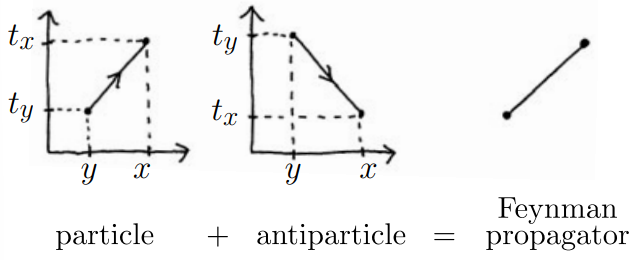
\includegraphics[width=0.6\linewidth]{Immagini/rappr. grafica prop. feynman.png}
    \caption{rappresentazione grafica del propagatore di Feynman vista come somma dei contributi di particella ed antiparticella.}
    \label{fig: rappr. grafica prop. feynman}
\end{figure}

La discussione fatta per i campi scalari carichi può chiaramente essere ripetuta per il caso più semplice dei campi scalari neutri dati da \eqref{eq: campo scalare quantizzato}, in tal caso il propagatore di Feynman è semplicemente 
\begin{equation}
    \Delta(x,y) = \mybrakett{0}{T[\hatphi(x)\hatphi(y)]}{0},
\end{equation}
la cui espressione esplicita è la medesima trovata in \eqref{eq: propagatore libero campo scalare carico (Theta)}.

\subsubsection{Causalità}
Considerando per semplicità il caso dei campi scalari neutri, l'ampiezza di probabilità che una particella si propaghi da un punto $y^\mu$ dello spaziotempo ad un altro $x^\mu$ è, come detto prima, data dall'integrale Lorentz invariante
\begin{equation}
\label{eq: propagatore libero campo scalare carico parziale}
    D(x - y) = \int\frac{d^3k}{(2\pi)^3}\frac{1}{(2\omega_k)}e^{-ik_\mu(x^\mu - y^\mu)}.
\end{equation}
Ci si concentra ora sul risolvere questo integrale per particolari valori della differenza $x^\mu - y^\mu$. Si supponga quindi che la differenza $x^\mu - y^\mu$ sia puramente temporale, ossia che $x^0 - y^0 = t$ e che $\vx -\vy = \bm{0}$, in questo caso si ha
\begin{equation}
    \begin{split}
        D(x - y) &= \frac{4\pi}{(2\pi)^{3}}\int_\R dk\,\frac{p^2}{2\sqrt{p^2 + m^2}}e^{-i\sqrt{p^2 + m^2}t} \\
        &=\frac{1}{4\pi^2}\int_m^\infty dE\, \sqrt{E^2 - m^2}e^{-iEt} \\
        &\overset{t\to\infty}{\simeq} e^{-imt}.
    \end{split}
\end{equation}
Ora si consideri invece che la distanza spaziotemporale $x^\mu - y^\mu$ sia puramente spaziale, ossia che $x^0 - y^0 = 0$ e che $\vx -\vy = \bm{r}$, in questo caso si ha
\begin{equation}
    \begin{split}
        D(x - y) &= \int\frac{d^3k}{(2\pi)^3}\frac{1}{2\omega_k}e^{ik_ir^i} \\
        &= \frac{2\pi}{(2\pi)^3}\int_0^\infty dk\,\frac{p^2}{2\omega_k}\frac{e^{i|\vp||\vr|} - e^{-i|\vp||\vr|}}{i|\vp||\vr|} \\ 
        &= \frac{-i}{2(2\pi)^2|\vr|}\int_\R \frac{|\vp|e^{i|\vp||\vr|}}{\sqrt{p^2 + m^2}}\\
        &=\frac{1}{4\pi^2|\vr|}\int_m^\infty d\rho\,\frac{\rho e^{-\rho|\vr|}}{\sqrt{\rho^2 - m^2}} \\
        &\overset{r\to\infty}{\simeq} e^{-mr},
    \end{split}
\end{equation}
dove, considerando l'integrando come una funzione complessa di $|\vp|$, si è definito $\rho = -i|\vp|$ e si è valutato l'integrale modificando il cammino di integrazione a causa dei poli in $\pm im$ scegliendo di chiuderlo nel semipiano immaginario positivo. Questi due risultati affermano che l'ampiezza di probabilità fuori dal cono luce decresce esponenzialmente ma non è identicamente nulla. Tuttavia, per discutere la causalità si dovrebbe in realtà chiedersi non se le particelle possono propagarsi seguendo specifici intervalli, ma se una misura effettuata in un punto dello spaziotempo può influenzare una misura effettuata in un altro punto separato dal primo da una distanza di tipo spazio. L'elemento più semplice che si può misurare è proprio il campo $\hatphi(x)$, quindi si considera il commutatore $\comm{\hatphi(x)}{\hatphi(y)}$: se questo si annulla, allora una misura non può influenzarne un'altra. Chiaramente, dalle condizioni \eqref{eq: regole di commutazione campo scalare quantizzato} è già noto che il commutatore in questione si annulli per $x^0  = y^0$, si svolge quindi il calcolo più generale
\begin{equation}
    \begin{split}
        \comm{\hatphi(x)}{\hatphi(y)} &= \iint\frac{d^3k\,d^3k'}{(2\pi)^{3}(2\omega_k)^{1/2}(2\omega_{k'})^{1/2}}\times \\
        &\times\comm{\hata_k e^{-ik_\mu x^\mu} + \hataT_k e^{ik_\mu x^\mu}}{\hata_{k'} e^{ik'_\mu y^\mu} + \hata_{k'} e^{ik'_\mu y^\mu}} \\
        &= \int\frac{d^3k}{(2\pi)^3}\frac{1}{2\omega_k}(e^{-ik_\mu(x^\mu - y^\mu)} - e^{ik_\mu(x^\mu - y^\mu)}) \\
        &= D(x - y) - D(y - x),
    \end{split}
\end{equation}
dove si sono usate le regole di commutazione \eqref{eq: regole commutazione operatori a campo scalare}. Quando l'intervallo è di tipo spazio per cui $(x^\mu - y^\mu)^2 < 0$ è possibile effettuare una trasformazione di Lorentz sul secondo termine, dato che ogni termine è Lorentz invariante in modo indipendente, passando da $(x^\mu - y^\mu)\to-(x^\mu - y^\mu)$. In questo modo, la differenza $D(x - y) - D(y - x)$ si annulla e la causalità è conservata. Si osservi inoltre che se $(x^\mu - y^\mu)^2 > 0$ non esiste una trasformazione di Lorentz continua che permetta il passaggio $(x^\mu - y^\mu)\to-(x^\mu - y^\mu)$, in questo caso l'ampiezza di probabilità è diversa da zero, in particolare per $\vx - \vy = \bm{0}$ è circa $(e^{-imt} - e^{imt})$. Dunque, si conclude che nessuna misura in una teoria di campo scalare può influenzare un'altra misura fuori dal cono luce. 

Un discorso analogo può essere fatto nel caso di campi scalari carichi, dove il campo $\hatphi(x)$ genera particelle cariche positivamente e distrugge particelle caricate negativamente, mentre il suo aggiunto $\hatphid(x)$ effettua le operazioni opposte. Quindi, il commutatore $\comm{\hatphi(x)}{\hatphid(y)}$ avrà contributi non nulli che si devono però annullare fuori dal cono luce in modo da preservare la causalità. I due contributi sono interpretati nel medesimo modo in cui si sono interpretati $D(x - y)$ e $D(y - x)$, solo con l'aggiunta della carica: il primo rappresenta la propagazione di una particella carica negativamente da $y^\mu$ a $x^\mu$, mentre il secondo quella di una carica positivamente  da $x^\mu$ a $y^\mu$. Affinché questi due processi generino ampiezze di probabilità opposte è necessario che entrambe le particelle esistano e che abbiano la medesima massa. In Teoria dei campi quindi, la causalità richiede che per ogni particella esista una corrispondente antiparticella avente la medesima massa e numeri quantici opposti, in questo caso la carica elettrica. Per un campo scalare neutro, ogni particella è l'antiparticella di se stessa.

\section{Propagatore di Feynman}
Si vuole ora determinare l'espressione esplicita del propagatore di Feynman ricavato nell'equazione \eqref{eq: propagatore libero campo scalare carico (Theta)}. In realtà, convenzionalmente si pone $\Delta(x,y) = i\Delta_F(x,y)$, dove $\Delta_F(x,y)$ prende effettivamente il nome di propagatore di Feynman. Quindi, prima di tutto si pone $z^\mu \equiv x^\mu - y^\mu$ e si scrive il propagatore di Feynman usando la normalizzazione Lorentz invariante
\begin{equation}
\label{eq: propagatore di Feynman norm. Lorentz invariante}
    i\Delta_F(x,y) = \int \frac{d^4p}{(2\pi)^3}\,\Theta(p_0)\delta(p^2 - m^2)[\Theta(z^0)e^{-ip_\mu z^\mu} + \Theta(-z^0)e^{ip_\mu z^\mu}]
\end{equation}
e si osserva come questa sia una definizione a tratti a causa delle Theta di Heaviside $\Theta(p_0)$ e $\Theta(\pm z^0)$. Per ``rimuovere'' questi contributi si considera l'espressione integrale della Theta ricavabile tramite il teorema di Cauchy
\begin{equation}
\label{eq: espressione integrale Theta Heaviside}
    \Theta(z^0) = \lim_{\epsilon\to0^+}\frac{1}{2i\pi}\int_\R d\tau\,\frac{e^{i\tau z^0}}{\tau - i\epsilon}.
\end{equation}
Per semplicità nel seguito si trascurano i termini $\mathcal{O}(\epsilon^2)$ e si sottintende il limite per $\epsilon\to0^+$. Sostituendo l'espressione \eqref{eq: espressione integrale Theta Heaviside} nella \eqref{eq: propagatore di Feynman norm. Lorentz invariante} si ottiene
\begin{equation}
    \begin{split}
        i\Delta_F(x,y) &= \int \frac{d^4p}{i(2\pi)^4}\int_\R d\tau\,\Theta(p_0)\delta(p^2 - m^2) \\
        &\times\bigg[\frac{e^{-i(p_\mu z^\mu - \tau z^0)}}{\tau - i\epsilon} + \frac{e^{i(p_\mu z^\mu - \tau z^0)}}{\tau - i\epsilon}\bigg].
    \end{split}
\end{equation}
Considerando il secondo termine nella parentesi quadra, si effettua un cambio di variabili $p_\mu \to -p_\mu$ e $\tau \to -\tau$ in modo da avere
\begin{equation}
    \Theta(p_0) \to \Theta(-p_0),\quad 
        \dfrac{e^{i(p_\mu z^\mu - \tau z^0)}}{\tau - i\epsilon} \to \dfrac{e^{-i(p_0z^0 - p_i z^i - \tau z^0)}}{-\tau - i\epsilon} \equiv \dfrac{e^{-ip'_\mu z^\mu}}{-\tau - i\epsilon},
\end{equation}
dove si è definito il quadrimpulso $p_\mu' = (p'_0,p'_i) = (p_0 - \tau,p_i)$, il quale si deve notare non soddisfa l'equazione di mass-shell in quanto ora $\vp'^{\,2} + m^2 = \omega_{p'}^2$. Con questa definizione di $p_\mu'$ si possono anche riscrivere
\begin{align}
    \delta(p^2 - m^2) &= \delta(p_0^2 - p_i^2 - m^2) \notag\\
    &= \delta((p'_0 + \tau)^2 - p_i'^{\,2} - m^2) \\
    &= \frac{\delta(p'_0 + \tau + \omega_{p'})}{2\omega_{p'}} + \frac{\delta(p'_0 + \tau - \omega_{p'})}{2\omega_{p'}}, \notag\\
    \Theta(\pm p_0) &= \Theta(\pm p_0' \pm \tau).
\end{align}
Dunque, si ottiene
\begin{equation}
    \begin{split}
        i\Delta_F(x,y) &= \int\frac{d^4p'}{i(2\pi)^4}\int_\R d\tau\,e^{-ip_\mu'z^\mu}\bigg[\frac{\Theta(p_0' + \tau)}{\tau - i\epsilon} + \frac{\Theta(-p_0' - \tau)}{-\tau - i\epsilon}\bigg]\times \\
        &\times\bigg[\frac{\delta(p'_0 + \tau + \omega_{p'})}{2\omega_{p'}} + \frac{\delta(p'_0 + \tau - \omega_{p'})}{2\omega_{p'}}\bigg] \\
        &= \int\frac{d^4p'}{i(2\pi)^4}\int_\R d\tau\,e^{-ip_\mu'z^\mu}\bigg[\frac{\delta(p'_0 + \tau + \omega_{p'})}{2\omega_{p'}}\frac{\Theta(-p_0' - \tau)}{-\tau - i\epsilon}+ \\
        &+ \frac{\delta(p'_0 + \tau - \omega_{p'})}{2\omega_{p'}}\frac{\Theta(p_0' + \tau)}{\tau - i\epsilon}\bigg].
    \end{split}
\end{equation}
Adesso, sfruttando le delta di Dirac e integrando su $d\tau$ si ha
\begin{equation}
    \begin{split}
        i\Delta_F(x,y) &= \int\frac{d^4p'}{i(2\pi)^4}\frac{e^{-ip_\mu'z^\mu}}{2\omega_{p'}}\bigg(\frac{1}{p_0' + \omega_{p'} - i\epsilon} + \frac{1}{-p_0' + \omega_{p'} - i\epsilon}\bigg) \\
        &= \int\frac{d^4p'}{i(2\pi)^4}\frac{e^{-ip_\mu'z^\mu}}{2\omega_{p'}}\frac{2\omega_{p'} - 2i\epsilon}{(\omega_p' - i\epsilon)^2 - (p_0')^2} \\
        &= \int\frac{d^4p'}{i(2\pi)^4}\frac{e^{-ip_\mu'z^\mu}}{\omega_{p'}^2 - (p_0')^2},
    \end{split}
\end{equation}
che considerando la relazione $\omega_{p'}^2 - (p_0')^2 = p_i^2 + m^2 - (p_0')^2 = m^2 - p'^{\,2}$ e scalando $-2i\epsilon\omega_{p'}\to -i\epsilon$ permette di ottenere un'espressione per il propagatore di Feynman nello spazio delle coordinate
\begin{equation}
\label{eq: propagatore libero campo scalare carico}
    \Delta_F(x,y) = \int\frac{d^4p}{(2\pi)^4}\frac{e^{-ip_\mu'z^\mu}}{p^2 - m^2 + i\epsilon}.
\end{equation}
Nello spazio degli impulsi invece, tramite una trasformata di Fourier, il propagatore di Feynman assume la forma
\begin{equation}
\label{eq. propagatore libero campo scalare carico (spazio impulsi)}
    \tilde{\Delta}_F(p) = \frac{1}{p^2 - m^2 + i\epsilon}.
\end{equation}
In entrambi i risultati \eqref{eq: propagatore libero campo scalare carico} e \eqref{eq. propagatore libero campo scalare carico (spazio impulsi)}, il termine a denominatore $i\epsilon$ assume il ruolo fondamentale di preservare la causalità e dalla rappresentazione integrale della Theta di Heaviside \eqref{eq: espressione integrale Theta Heaviside}, facendo attenzione a considerare il corretto contorno di integrazione dal punto di vista fisico tra le quattro scelte matematicamente equivalenti possibili.

Si può infine verificare che il propagatore in \eqref{eq: propagatore libero campo scalare carico} è la funzione di Green dell'operatore di Klein-Gordon $(\square + m^2)$, infatti
\begin{equation}
    (\square + m^2)\Delta_F(x,y) = \int\frac{d^4p}{(2\pi)^4}\frac{-p^2 + m^2}{p^2 - m^2 + i\epsilon}e^{-p_\mu z^\mu},
\end{equation}
considerando poi che il fattore $i\epsilon$ può essere mandato a zero grazie al limite sottinteso per $\epsilon\to0^+$ si ha proprio
\begin{equation}
     (\square + m^2)\Delta_F(x,y) = -\int\frac{d^4p}{(2\pi)^4}e^{-p_\mu z^\mu} = -\delta^4(x - y).
\end{equation}
In aggiunta, nel caso dei campi vettoriali, che descrivono particelle come il fotone, si definisce il propagatore come
\begin{equation}
    \Delta(x,y) = \frac{1}{k^2 - i\epsilon}.
\end{equation}
Invece, per il campo spinoriale di Dirac si definisce il propagatore come
\begin{equation}
    iS_F(x,y) = \mybrakett{0}{T[\hatpsi(x)\hatpsib(y)]}{0}
\end{equation}
che, seguendo un processo analogo a quanto fatto per il campo scalare anche se più tortuoso a causa dell'algebra delle matrici $\gamma^\mu$, ha come forma esplicita nello spazio dello coordinate 
\begin{equation}
\label{eq: propagatore campo spinoriale}
    S_F(x,y) = \int\frac{d^4p}{(2\pi)^4}\frac{\slp + m}{p^2 - m^2 + i\epsilon},
\end{equation}
mentre nello spazio degli impulsi risulta essere
\begin{equation}
    \tilde{S}_F(p) = \frac{\slp + m}{p^2 - m^2} = \frac{i}{\slp - m}. 
\end{equation}
\chapter{Teoria delle perturbazioni}
Fino ad ora si sono discusse teoria di campo libere che danno una descrizione approssimata di molte particelle trovate in Natura. Tuttavia, stati di particella libera sono autostati dell'hamiltoniana e non si è parlato né di interazione né di scattering. In modo da ottenere una descrizione più accurata del mondo reale si devono necessariamente includere nuovi termini non lineari nell'hamitoniana o nella lagrangiana che accoppiano differenti modi di Fourier, e le particelle che li occupano, l'uno con l'altro. Per conservare la causalità, si insiste sulla condizione che questi nuovi termini devono includere solamente prodotti dei campi e dello loro derivate calcolate nello stesso punto dello spaziotempo. Quindi, l'hamiltoniana che include i termini descriventi l'interazione ha la forma
\begin{equation}
    \hatH' = \int d^3x\,\SH'[\hatphi(x),\p_\mu\hatphi(x)] = -\int d^3x\,\dL'[\hatphi(x),\p_\mu\hatphi(x)].
\end{equation}
Si intende ora studiare la Teoria delle perturbazioni per campi interagenti con l'obiettivo di arrivare ad un formalismo che permetta di visualizzare le serie perturbative come processi dello spaziotempo. Pur non avendo necessità di riformulare la Meccanica quantistica, si intende derivare una ``nuova'' Teoria delle perturbazioni dipendenti dal tempo conveniente per una teoria di campo. Il risultato a cui si intende arrivare è il calcolo delle sezioni d'urto dei processi di scattering e le frequenze di decadimento, ma per ora ci si concentra sul calcolare la più semplice, anche se più astratta, funzioni di Green a due punti 
\begin{equation}
    \mybrakett{\Omega}{T[\hatphi(x)\hatphi(y)]}{\Omega}.
\end{equation}
Per una teoria libera si era determinato che il propagatore di un campo scalare, sia carico che neutro, ha la forma trovata nell'equazione \eqref{eq: propagatore libero campo scalare carico}, quindi si vuole capire come tale espressione cambi in una teoria interagente e quale sia la relazione che la lega al propagatore libero. Per farlo, prima di tutto si scrive l'hamiltoniana del sistema come la somma tra quella libera e quella di interazione
\begin{equation}
    \hatH = \hatH_0 + \hatH',\quad \hatH' \ll 1,
\end{equation}
dove la condizione imposta sull'hamiltoniana di interazione è fondamentale per sviluppare una teoria perturbativa, infatti in questo modo si sta considerando un'interazione ``piccola'' e presente per un tempo molto limitato, in modo da poter sviluppare in serie i termini di interazione. Tale condizione è anche legata al fatto che in generale in Teoria dei campi le interazioni sono descritte come lo scambio di particelle ``virtuali'', ossia particelle che non rispettano l'equazione di mass-shell della Relatività speciale violando quindi la conservazione dell'energia; potrebbe sembrare impossibile, ma in realtà questa violazione è giustificata dal fatto che queste particelle vivono per un tempo tale da soddisfare la relazione di indeterminazione tra energia e tempo $\Delta E \Delta t  \simeq \hbar$. Ora per descrivere l'evoluzione temporale di stati ed operatori si fa uso di una particolare rappresentazione detta ``di interazione'' in cui gli stati $\ket{\psi_I}$ evolvono unicamente con l'hamiltoniana di interazione $\hatH'$, mentre gli operatori $\hatO$ evolvono unicamente con l'hamiltoniana libera $\hatH_0$; in questo modo gli operatori evolvono secondo
\begin{equation}
    \hatO_I(t) = e^{i\hatH_0t}\hatO e^{-i\hatH_0t}
\end{equation}
ottenendo così un'equazione del moto alla Heisenberg per l'hamiltoniana libera
\begin{equation}
    i\frac{d\hatO_I}{dt} = \comm{\hatO_I(t)}{\hatH_0},
\end{equation}
invece gli stati soddisfano l'equazione di Schr\"odinger per l'hamiltoniana di interazione
\begin{equation}
    i\frac{\p}{\p t}\ket{\psi_I(t)} = \hatH'_I\ket{\psi_I(t)},\quad \hatH_I' = e^{i\hatH_0t}\hatH' e^{-i\hatH_0t}.
\end{equation}
Stabilita l'evoluzione temporale degli operatori, si considera un generico elemento di matrice nella rappresentazione di Schr\"odinger e lo si confronta con uno in quella di interazione in modo da verificare che queste rappresentazioni siano equivalenti
\begin{equation}
    \begin{split}
        \mybrakett{\phi(t)}{\hatO}{\psi(t)}&=\mybrakett{\phi(0)}{\hatU^\dagger(t,0)\hatO\hatU(t,0)}{\psi(0)} \\
        &=\mybrakett{\phi(0)}{e^{i\hatH t}\hatO e^{-i\hatH t}}{\psi(0)} \\
        &=\mybrakett{\phi(0)}{e^{i\hatH' t}e^{i\hatH_0 t}\hatO e^{-i\hatH_0 t}e^{-i\hatH' t}}{\psi(0)} \\
        &=\mybrakett{\phi_I(t)}{e^{i\hatH_0 t}\hatO e^{-i\hatH_0 t}}{\psi_I(t)},
    \end{split}
\end{equation}
quindi i valori medi di ogni elemento di matrice sono gli stessi in qualsiasi rappresentazione
\begin{equation}
    \underbrace{\mybrakett{\phi(t)}{\hatO}{\psi(t)}}_{\substack{Schr\ddot{o}dinger\\picture}}\equiv\underbrace{\mybrakett{\phi_I(t)}{e^{i\hatH_0t}\hatO e^{-i\hatH_0t}}{\psi_I(t)}}_{\substack{interaction\\picture}}.
\end{equation}
\begin{obs}
    Al tempo $t=0$ tutte le rappresentazioni, Schr\"odinger, Heisenberg ed interazione, coincidono.
\end{obs}
La rappresentazione di interazione è utile in quanto l'hamiltoniana di interazione $\hatH'$ è nulla all'inizio e alla fine del processo. Infatti, si supponga che $\hatH'$ si ``accenda'' e si ``spenga'' in modo continuo senza interruzioni. Quando $\hatH_I=0$ l'unica rappresentazione presente è quella di Heisenberg per l'hamiltoniana libera $\hatH_0$. Quindi, gli autostati di $\hatH_0$ sono $\ket{\psi_I(\pm\infty)}$, i quali possono essere costruiti a partire dallo stato di vuoto $\sv$ applicando gli operatori di creazione o distruzione. Inoltre, l'hamiltoniana di interazione è diversa da zero solo durante il breve intervallo di tempo in cui avviene l'interazione tra particelle, per poi tornare nuovamente a zero, quindi $\hatH'=0$ per $t\to\pm\infty$. In questo modo, è possibile dare una rappresentazione funzionale dell'hamiltoniana di interazione
\begin{equation}
    \hatH_I(t)=\lambda(t)\hatH'.
\end{equation}
\begin{figure}[h]
    \centering
    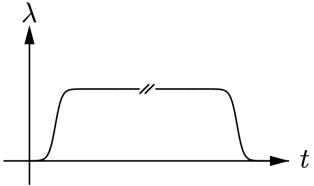
\includegraphics[width=0.5\linewidth]{Immagini/rappr. ham. int.png}
    \caption{rappresentazione funzionale dell'hamiltoniana di interazione.}
    \label{fig: rappr. ham. int.}
\end{figure}

Ricapitolando, gli stati evolvono nel tempo solo durante il periodo in cui avviene l'interazione secondo $\hatH'$, o meglio $\hatH_I$, nel quale $\hatH_I\neq0$; al di fuori di tale intervallo gli stati sono stazionari, mentre gli operatori evolvono nel tempo secondo $\hatH_0$.

Quindi, essendo i campi degli operatori la loro evoluzione temporale in rappresentazione di Heisenberg è data da
\begin{equation}
    \hatphi(\vx,t) = e^{i\hatH(t - t_0)}\hatphi(\vx,t_0)e^{-i\hatH(t - t_0)},
\end{equation}
scegliendo un istante di tempo fissato $t_0$ è possibile esprimere il campo tramite la sua espressione esplicita \eqref{eq: campo scalare quantizzato} in termini di operatori di creazione e distruzione, in particolare per $\lambda(t) = 0$, l'hamiltoniana $\hatH$ si riduce ad $\hatH_0$ e l'evoluzione temporale del campo in rappresentazione di interazione, come ci si aspetta, è
\begin{equation}
    \hatphi_I(\vx,t) \equiv e^{i\hatH_0(t - t_0)}\hatphi(\vx,t_0)e^{-i\hatH_0(t - t_0)};
\end{equation}
quando $\lambda(t) \ll 1$ questa espressione continua a restituire la parte più importante della dipendenza temporale del campo $\hatphi(x)$ e quindi è possibile usarla in una teoria perturbativa. Adesso si deve esprimere il campo $\hatphi(x)$ in termini di $\hatphi_I(x)$, quindi
\begin{equation}
    \begin{split}
        \hatphi(x) &= e^{i\hatH(t - t_0)}e^{-i\hatH_0(t - t_0)}\hatphi_I(x)e^{i\hatH_0(t - t_0)}e^{i\hatH(t - t_0)} \\
        &= \hatU^\dg_I(t,t_0)\hatphi_I(t)\hatU_I(t,t_0),
    \end{split}
\end{equation}
dove si è definito l'operazione di evoluzione temporale in rappresentazione di interazione $\hatU_I(t,t_0)$ come
\begin{equation}
    \hatU_I(t,t_0) := e^{i\hatH_0(t - t_0)}e^{-i\hatH(t - t_0)}.
\end{equation}
Anche $\hatU_I(t,t_0)$ deve essere espresso in termini di $\hatphi_I(x)$ di cui si conosce la forma esplicita. Per farlo, si osserva che $\hatU(t,t_0)$ è soluzione, con condizione iniziale $\hatU_I(t_0,t_0) = 1$, dall'equazione di Schr\"odinger
\begin{equation}
    \begin{split}
        i\frac{\p}{\p t}\hatU_I(t,t_0) &= e^{i\hatH_0(t - t_0)}(\hatH - \hatH_0)e^{-i\hatH(t-t_0)} \\
        &= e^{i\hatH_0(t - t_0)}\hatH'e^{-i\hatH(t - t_0)} \\
        &= e^{i\hatH_0(t - t_0)}\hatH'e^{-i\hatH_0(t - t_0)}e^{i\hatH_0(t - t_0)}e^{-i\hatH(t - t_0)} \\
        &= \hatH_I'(t)\hatU_I(t,t_0).
    \end{split}
\end{equation}
La soluzione di tale equazione non è semplicemente dato dall'esponenziale $\hatU(t,t_0) = \exp{(-i\int_{t_0}^t\hatH_I'(t')\,dt')}$ dato che l'hamiltoniana di interazione non commuta a tempi diversi, infatti in verità si ha
\begin{equation}
    \hatU(t,t_0) = 1 + (-i)\int_{t_0}^tdt_1\,\hatH_I'(t_1) + (-i)^2 \int_{t_0}^t\int_{t_0}^{t_1}dt_1\,dt_2\,\hatH_I'(t_1)\hatH_I'(t_2) + \cdots,
\end{equation}
che può essere riscritta tramite l'operatore di ordinamento temporale \eqref{eq: ordinamento temporale} nella forma più compatta
\begin{equation}
    \hatU(t,t_0) = T\bigg[\exp{\bigg(-i\int_{t_0}^tdt'\,\hatH'_I(t')\bigg)}\bigg],
\end{equation}
dove l'operatore $T$ è definito come la serie di Taylor avente ogni termine ordinato temporalmente. 

Si vuole adesso trovare una relazione tra lo stato fondamentale interagente $\kO$ e lo stato di vuoto $\sv$. Siccome l'energia minima di una teoria libera è posta a zero, allora $\hatH_0\sv = 0$. Considerando il termine di interazione $\hatH = \hatH_0 + \hatH'$, si definiscono ${\ket{n}}$ come gli autostati di $\hatH$ dotati di una relazione di completezza 
\begin{equation}
    \nsum_n\ket{n}\bra{n} = \MI,
\end{equation}
tra questi autostati esiste uno stato $\kO$ che appunto rappresenta lo stato fondamentale della teoria interagente tale per cui
\begin{equation}
    \hatH\kO = E_0\kO.
\end{equation}
Lo stato $\kO$ può essere espresso come una sovrapposizione lineare, potenzialmente infinita, di autostati dell'impulso di $\hatH_0$. Tra tutti questi ulteriori autostati di $\hatH_0$ è presente anche lo stato di vuoto $\sv$, per cui $\kO$ è parzialmente sovrapposto a $\sv$ e quindi $\mybraket{\Omega}{0} \neq 0$. Per isolare $\kO$ si parte pertanto dall'evolvere lo stato $\sv$ tramite $\hatH$ per un tempo $T$ ottenendo
\begin{equation}
    \begin{split}
        e^{-i\hatH T}\sv &= e^{-i\hatH T}\nsum_n\ket{n}\mybraket{n}{0} \\
        &= \nsum_n e^{-iE_nT}\ket{n}\mybraket{n}{0} \\
        &= e^{-iE_0T}\kO\mybraket{\Omega}{0} + \nsum_{n\neq0}e^{-iE_nT}\ket{\mybraket{n}{0}}.
    \end{split}
\end{equation}
Dato che per ogni $n\neq0$, $E_n > E_0$, allora ci si può sbarazzare dei termini con $n\neq0$ considerando il limite complesso per $T\to\infty(1 - i\epsilon)$ e, dato che il termine con $e^{iE_0t}$ è quello che decresce più lentamente, si ha
\begin{equation}
    \kO = \lim_{T\to\infty(1 - i\epsilon)}(e^{-iE_0T}\mybraket{\Omega}{0})^{-1}e^{-i\hatH T}\sv.
\end{equation}
Dato che $T\to\infty(1 - i\epsilon) \equiv \infty^\C$, allora si può considerare una traslazione temporale $T\to T + t_0$, con $t_0\in\R$, in questo modo
\begin{equation}
    \begin{split}
        \kO &= \lim_{T\to\infty^\C}(e^{-iE_0(T + t_0)}\mybraket{\Omega}{0})^{-1}e^{-i\hatH (T + t_0)}\sv \\
        &= \lim_{T\to\infty^\C}(e^{-iE_0(t_0 - (-T))}\mybraket{\Omega}{0})^{-1}e^{-i\hatH (t_0 - (-T))}\sv \\
        &= \lim_{T\to\infty^\C}(e^{-iE_0(t_0 - (-T))}\mybraket{\Omega}{0})^{-1}e^{-i\hatH (t_0 - (-T))}e^{i\hatH_0(t_0 - (-T))}\sv \\
        &= \lim_{T\to\infty^\C}(e^{-iE_0(t_0 - (-T))}\mybraket{\Omega}{0})^{-1}\hatU(t_0,-T)\sv,
    \end{split}
\end{equation}
dove la definizione $\hatU(t_0,-T) := e^{-i\hatH (t_0 - (-T))}e^{i\hatH_0(t_0 - (-T))}$ vale in quanto per $T\to\infty^\C$ si ha $\hatH\simeq\hatH_0$ e $\hatH'\to0$. Analogamente, si può esprimere 
\begin{equation}
    \bO = \lim_{T\to\infty^\C}\bra{0}\hatU(T,t_0)(e^{-iE_0(T - t_0)}\mybraket{0}{\Omega})^{-1}.
\end{equation}
Ora che sono note le espressioni degli stati $\kO$ e $\bO$ in funzione di $\sv$ e $\bra{0}$ insieme a quelle dei campi $\hatphi(x)$ in funzione di $\hatphi_I(x)$ è possibile determinare la forma del propagatore interagente, quindi
\begin{equation}
    \begin{split}
        \mybrakett{\Omega}{T[\hatphi(x)\hatphi(y)]}{\Omega} &= \lim_{T\to\infty^\C}(|\mybraket{0}{\Omega}|^2e^{-2iE_0T})^{-1} \times \\
        &\times\mybrakett{0}{\hatU(T,x^0)\hatphi_I(x)\hatU(x^0,y^0)\hatphi_I(y)\hatU(y^0,-T)}{0},
    \end{split}
\end{equation}
dove per il momento si è supposto che $x^0 > y^0 > t_0$. Adesso dividendo per la normalizzazione dello stato fondamentale 
\begin{equation}
    \mybraket{\Omega}{\Omega} = (|\mybraket{0}{\Omega}|^2e^{-2iE_0T})^{-1}\mybrakett{0}{\hatU(T,t_0)\hatU(t_0,-T)}{0} = 1,
\end{equation}
si ottiene 
\begin{equation}
    \mybrakett{\Omega}{T[\hatphi(x)\hatphi(y)]}{\Omega} = \lim_{T\to\infty^\C}\frac{\mybrakett{0}{\hatU(T,x^0)\hatphi_I(x)\hatU(x^0,y^0)\hatphi_I(y)\hatU(y^0,-T)}{0}}{\mybrakett{0}{\hatU(T,t_0)\hatU(t_0,-T)}{0}}.
\end{equation}
Quest'ultima però non è ancora l'espressione completa dato che non si sta rispettando necessariamente la causalità, come al solito si deve introdurre l'operatore di ordinamento temporale per rispettarla ottenendo finalmente l'espressione del propagatore di una teoria interagente in funzione dello stato di vuoto di una teoria libera
\begin{equation}
\label{eq: teorema di Gell-Mann - Low}
    \mybrakett{\Omega}{T[\hatphi(x)\hatphi(y)]}{\Omega} = \lim_{T\to\infty^\C}\frac{\mybrakett{0}{T[\hatphi_I(x)\hatphi_I(y)\exp{(-i\int_{-T}^Tdt\,\hatH_I(t))}]}{0}}{\mybrakett{0}{T[\exp{(-i\int_{-T}^Tdt\,\hatH_I(t)}]}{0}}.
\end{equation}
L'incredibile e fondamentale risultato mostrato nella \eqref{eq: teorema di Gell-Mann - Low} è codificato formalmente nel teorema di Gell-Mann - Low nella Teoria dei campi. Il risultato trovato è chiaramente estendibile ad un numero arbitrario di campi; per ogni fattore ulteriore $\hatphi$ nel membro sinistro si aggiunge un fattore $\hatphi_I$ in quello di destra. Oltre ad essere un'espressione esatta, è anche adatta per svolgere calcoli perturbativi: serve solamente troncare la serie di Taylor degli esponenziali all'ordine a cui si è interessati.

\section{Teorema di Wick}
Le quantità che spesso si devono calcolare per determinare le ampiezze di scattering $\amp$ di una determinata teoria sono valori di aspettazione di un prodotto T-ordinato di un certo numero di campi, ossia oggetti del tipo
\begin{equation}
    \mybrakett{0}{T[\hatphi_I(x_1)\cdots\hatphi_I(x_n)]}{0}.
\end{equation}
Questo tipo di calcoli è in generale molto complesso, ma il teorema di Wick semplifica notevolmente la procedura. Questo mette in relazione il valore di aspettazione sullo stato di vuoto del prodotto T-ordinato con quello del prodotto ``normal ordered'', il quale è sempre nullo dato che l'ordinamento normale pone gli operatori di distruzione a destra e quelli di creazione a sinistra, rendendo il valore di aspettazione sul vuoto nullo.

Quindi, si parte considerando, ad esempio, l'espressione dell'operatore di campo $\hatphi$ in \eqref{eq: campo scalare quantizzato} e osservando che è composto da due parti, una di distruzione e una di creazione, pertanto $\hatphi$ può essere scritto come la somma di tali parti $\hatphi=\hatphi^++\hatphi^-$, in modo da avere $\hatphi^-\sv=\bra{0}\hatphi^+=0$ e quindi definite come
\begin{align}
\label{componenti campo + e -}
    \hatphi^+(x) &= \int\frac{d^3k}{(2\pi)^{3/2}}\frac{1}{(2\omega_k)^{1/2}}\hata_k^\dg e^{ik_\mu x^\mu}, \\
    \hatphi^-(x) &= \int\frac{d^3k}{(2\pi)^{3/2}}\frac{1}{(2\omega_k)^{1/2}}\hata_ke^{-ik_\mu x^\mu}.
\end{align}

Si consideri ora il caso più semplice di due operatori di campo $\hatphi_A$ e $\hatphi_B$. Il loro prodotto è dato da 
\begin{equation}
    \hatphi_A\hatphi_B=(\hatphi_A^++\hatphi_A^-)(\hatphi_B^++\hatphi_B^-)=\hatphi_A^+\hatphi_B^++\hatphi_A^-\hatphi_B^-+\hatphi_A^+\hatphi_B^-+\hatphi_A^-\hatphi_B^+.
\end{equation}
Nel caso di prodotto normalmente ordinato si ha
\begin{equation}
    N[\hatphi_A\hatphi_B]=\hatphi_A^+\hatphi_B^++\hatphi_A^-\hatphi_B^-+\hatphi_A^+\hatphi_B^-+\hatphi_B^+\hatphi_A^-.
\end{equation}
Il passo fondamentale è notare che la differenza tra questi due prodotti è
\begin{equation}
    \hatphi_A\hatphi_B-N[\hatphi_A\hatphi_B=\comm{\hatphi_A^-}{\hatphi_B^+}.
\end{equation}
Ricordando che $\hatphi_A$ e $\hatphi_B$ sono operatori di campo, il loro prodotto deve essere T-ordinato, quindi
\begin{equation}
    T[\hatphi_A(x^\mu)\hatphi_B(y^\mu)]=
    \begin{cases}
        \hatphi_A(x^\mu)\hatphi_B(y^\mu),\quad x^0>y^0 \\
        \hatphi_B(y^\mu)\hatphi_A(x^\mu),\quad y^0>x^0
    \end{cases}.
\end{equation}
Facendo ora la differenza tra il prodotto T-ordinato con quello normalmente ordinato si ottiene
\begin{equation}
    T[\hatphi_A(x^\mu)\hatphi_B(y^\mu)]-N(\hatphi_A\hatphi_B)=
    \begin{cases}
        \comm{\hatphi_A^-(x^\mu)}{\hatphi_B^+(y^\mu)},\quad x^0>y^0 \\
        \comm{\hatphi_B^-(y^\mu)}{\hatphi_A^+(x^\mu)},\quad y^0>x^0
    \end{cases}.
\end{equation}
Dato che il valore di aspettazione sullo stato di vuoto di un prodotto normalmente ordinato è sempre nullo, si può scrivere che il valore di aspettazione del prodotto T-ordinato come
\begin{equation}
    \mybrakett{0}{T[\hatphi_A(x^\mu)\hatphi_B(y^\mu)]}{0}=
    \begin{cases}
        \mybrakett{0}{\comm{\hatphi_A^-(x^\mu)}{\hatphi_B^+(y^\mu)}}{0},\quad x^0>y^0 \\
        \mybrakett{0}{\comm{\hatphi_B^-(y^\mu)}{\hatphi_A^+(x^\mu)}}{0},\quad y^0>x^0
    \end{cases}.
\end{equation}
In generale, si definisce la differenza tra il prodotto T-ordinato ed N-ordinato come una contrazione
\begin{equation}
\label{eq: definizione contrazione}
    \overbracket{\hatphi_A\hatphi_B}=T[\hatphi_A\hatphi_B]-N[\hatphi_A\hatphi_B].
\end{equation}
Dato che il prodotto normale non ha alcun effetto sul valore di aspettazione sullo stato di vuoto, si può scrivere che
\begin{equation}
    \label{eq: relazione tra contraz. e VEV}
    \overbracket{\hatphi_A\hatphi_B}=\overbracket{\hatphi_A\hatphi_B}\mybraket{0}{0}=\mybrakett{0}{\overbracket{\hatphi_A\hatphi_B}}{0}=\mybrakett{0}{T[\hatphi_A\hatphi_B]}{0}.
\end{equation}
Questo risultato può essere generalizzato con il seguente teorema.
\begin{teo}[teorema di Wick]
    Il prodotto T-ordinato di $n$ operatori $\hatphi_I(x_i) \equiv \hatphi_i$ è uguale al prodotto normale degli $n$ operatori più il prodotto normale della somma di tutti i possibili modi di contrarre gli operatori tra loro, ovvero
    \begin{equation}
        T[\hatphi_1\dots\hatphi_n] = N[\hatphi_1\dots\hatphi_n] + N[\mathrm{tutte\,le\,possibili\,contrazioni}].
    \end{equation}
\end{teo}
\begin{proof}
    Per prima cosa si nota che il prodotto T-ordinato di $n$ operatori di campo $\hatphi_I$ è invariante sotto lo scambio dei campi per definizione. Dato che i prodotti N-ordinati e le contrazioni sono invarianti sotto lo scambio dei campi è possibile, senza perdere di generalità, scegliere $x_{n + 1}^0 < x_i^0$ con $i\in\{1,\dots,n\}$. Assumendo che il teorema di Wick sia vero per $n$ operatori di campo si ha
    \begin{equation}
        \begin{split}
            T[\hatphi_1\dots\hatphi_{n+1}] &= T[\hatphi_1\dots\hatphi_n]\hatphi_{n+1} \\
            &= N[\hatphi_1\dots\hatphi_n]\hatphi_{n+1} + \sum_{\mathrm{perm}}\mybrakett{0}{T[\hatphi_1\hatphi_2]}{0}N[\hatphi_3\cdots\hatphi_n]\hatphi_{n+1}.
        \end{split}
    \end{equation}
    Finora $\hatphi_{n+1}$ è rimasto fuori dai prodotti N-ordinati; ora si deve operare in modo da portalo all'interno di tali prodotti. Per farlo si usano le definizioni \eqref{componenti campo + e -} e si nota che un prodotto N-ordinato ha sempre i campi $\hatphi^-$ a destra e i campi $\hatphi^+$ a sinsitra, per cui
    \begin{equation}
        N[\hatphi_1\cdots\hatphi_n] = \sum_{A,B}\prod_{i\in A}\prod_{j\in B}\hatphi^+_i\hatphi_j^-,
    \end{equation}
    dove $A$ e $B$ rappresentano le partizioni dell'insieme di $1,2,\dots,n$ elementi. Con questa notazione si può scrivere
    \begin{equation}
    \label{eq: prodotto N-ordinato Wick's proof}
        N[\hatphi_1\cdots\hatphi_m]\hatphi_{n+1} = \bigg[\sum_{A,B}\prod_{i\in A}\prod_{j\in B}\hatphi^+_i\hatphi_j^-\bigg](\hatphi^+_{n+1} + \hatphi^-_{n+1}).
    \end{equation}
    In quest'ultima espressione, $\hatphi^-_{n+1}$ si trova già nella posizione corretta per essere portato all'interno del prodotto N-ordinato, invece per $\hatphi^+_{n+1}$ il processo è più complesso. Ogni volta che $\hatphi^+_{n+1}$ viene commutato con uno dei campi $\hatphi^-$ genera un termine aggiuntivo, dovuto proprio al commutatore $\comm{\hatphi^-}{\hatphi^+}$ che in generale è un numero complesso. Per esempio, calcolando 
    \begin{equation}
        \begin{split}
            \hatphi^-(x)\hatphi^+(y) &= \int\frac{d^3k\,d^3k'}{(2\pi)^3(2\omega_k\omega_{k'})^{1/2}}\hata_k\hataT_{k'}e^{-ik_\mu x^\mu}e^{ik'_\mu y^\mu} \\
            &= \int\frac{d^3k\,d^3k'}{(2\pi)^3(2\omega_k\omega_{k'})^{1/2}}[\hataT_{k'}\hata_k + \delta^3(\vk - \vk')]e^{-ik_\mu x^\mu}e^{ik'_\mu y^\mu} \\
            &= \int\frac{d^3k\,d^3k'}{(2\pi)^3(2\omega_k\omega_{k'})^{1/2}}\hataT_{k'}\hata_ke^{-ik_\mu x^\mu}e^{ik'_\mu y^\mu} \\
            &+ \int\frac{d^3k}{(2\pi)^3}\frac{1}{(2\omega_k)}e^{-ik_\mu(x^\mu - y^\mu)}\\
            &=\hatphi^+(y)\hatphi^-(x) + \Delta,\quad \Delta\in\C,
        \end{split}
    \end{equation}
    e prendendone il valore di aspettazione sul vuoto
    \begin{equation}
        \mybrakett{0}{\hatphi^-(x)\hatphi^+(y)}{0} = \mybrakett{0}{\hatphi^+(y)\hatphi^-(x)}{0} + \Delta\mybraket{0}{0} = \Delta,
    \end{equation}
    si può trovare, combinando le ultime due relazioni, che
    \begin{equation}
        \hatphi^-(x)\hatphi^+(y) = \hatphi^+(y)\hatphi^-(x) + \mybrakett{0}{\hatphi^-(x)\hatphi^+(y)}{0}.
    \end{equation}
    Quindi, ad ogni permutazione del campo $\hatphi^+_{n+1}$ con un campo $\hatphi^-_j$ genera un termine $\mybrakett{0}{\hatphi^-_j\hatphi^+_{n+1}}{0}$. Quindi, tornando all'espressione di partenza \eqref{eq: prodotto N-ordinato Wick's proof}, si ha
    \begin{equation}
    \label{eq: Wick's proof}
        \begin{split}
            N[\hatphi_1\cdots\hatphi_n]\phi_{n+1} &= \sum_{A,B}\prod_{i\in A}\prod_{j\in B}(\hatphi^+_i\hatphi^-_j\hatphi^-_{n+1}) + \\
            &+ \sum_{A,B}\prod_{i\in A}\prod_{j\in B}(\phi^+_i\hatphi^+_{n+1}\hatphi^-_j) + \\
            &+ \sum_{k\in B}\prod_{j\neq k\in B}\hatphi^-_j\mybrakett{0}{\hatphi_k^-\hatphi_{n+1}^+}{0}.
        \end{split}
    \end{equation}
    Nell'espressione \eqref{eq: Wick's proof}, i primi due termini del secondo membro provengono dal corretto riposizionamento di $\hatphi^+_{n+1}$ all'interno del prodotto N-ordinato e ricostruiscono $ N[\hatphi_1\cdots\hatphi_{n+1}]$. Il terzo addendo invece rappresenta la somma di tutti i contributi ottenuti dallo scambio di posizione di $\hatphi^+_{n+1}$ con gli operatori $\hatphi^-_j$ necessari per far migrare $\hatphi^+_{n+1}$ sulla sinistra. Questi termini sono tutte le possibili contrazioni dei campi $\hatphi_i$ con $i=1,\dots,n$ a due a due, in tutti i modi possibili.
\end{proof}
Dal momento che la parte contratta è sempre un numero (in generale complesso) può essere portato fuori dall'ordinamento normale
\begin{equation}
    N[\contr{\hatphi_A\hatphi_B}\hatphi_C\hatphi_D]=\contr{\hatphi_A\hatphi_B}N[\hatphi_C\hatphi_D].
\end{equation}    
Quindi, quando si calcola il valore di aspettazione sul vuoto il contributo di ogni prodotto normale è nullo, quindi nel valore di aspettazione $\mybrakett{0}{T(\hatphi_A\hatphi_B\hatphi_C\cdots\hatphi_Z)}{0}$ gli unici contributi non nulli sono quelli che provengono dai termini in cui tutti gli operatori son contratti in tutti i modi possibili. Conseguenza di questo è che sono non nulli solo i valori di aspettazione sul vuoto dei prodotti di un numero pari di operatori, ossia
\begin{equation}
    \begin{split}
        \mybrakett{0}{T[\hatphi_A\hatphi_B\hatphi_C\cdots\hatphi_Z]}{0}&=\mybrakett{0}{T[\contr{\hatphi_A\hatphi_B}\contr{\hatphi_C\hatphi_D}\cdots\contr{\hatphi_Y\hatphi_Z}]}{0}+ \\
        &+\mybrakett{0}{T[\mathrlap{\overbracket{\phantom{\hatphi_A\hatphi_B\hatphi_C}}}\hatphi_A\underbracket{\hatphi_B\hatphi_C\hatphi_D}\cdots\contr{\hatphi_Y\hatphi_Z}]}{0}+ \\
        &+(\mathrm{tutte\,le\,altre\,possibili\,contrazioni}).
    \end{split}
\end{equation}
Usando la relazione \eqref{eq: relazione tra contraz. e VEV} si può scrivere 
\begin{equation}
    \begin{split}
        \mybrakett{0}{T[\hatphi_A\hatphi_B\cdots\hatphi_Z]}{0}&=\mybrakett{0}{T[\hatphi_A\hatphi_B]}{0}\mybrakett{0}{T[\hatphi_C\hatphi_D]}{0}\cdots\mybrakett{0}{T[\hatphi_Y\hatphi_Z]}{0}+ \\
            &+\mybrakett{0}{T[\hatphi_A\hatphi_C]}{0}\mybrakett{0}{T[\hatphi_B\hatphi_D]}{0}\cdots\mybrakett{0}{T[\hatphi_Y\hatphi_Z]}{0}+\\
            &+ \cdots.
    \end{split}
\end{equation}
Nel caso particolare del prodotto T-ordinato di solo due operatori di campo $\hatphi_I$, il suo valore di aspettazione sul vuoto è
\begin{equation}
    \begin{split}
        \mybrakett{0}{T[\hatphi_I(x)\hatphi(y)]}{0} &= \mybrakett{0}{\contr{\hatphi_I(x)\hatphi_I(y)}}{0} \\
        &= \mybraket{0}{0}\contr{\hatphi_I(x)\hatphi_I(y)} \\ 
        &= \contr{\hatphi_I(x)\hatphi_I(y)},
    \end{split}
\end{equation}
che coincide esattamente con la definizione di propagatore libero tra i punti dello spaziotempo $x$ e $y$ \eqref{eq: propagatore libero campo scalare carico parziale}.
\begin{ex}
    Un esempio molto importante riguarda quando gli operatori in questione sono quattro campi scalari. In tal caso
    \begin{equation}
        \begin{split}
            \mybrakett{0}{T[\hatphi(x_1)\hatphi(x_2)\hatphi(x_3)\hatphi(x_4)]}{0} &= D(x_1 - x_2)D(x_3 - x_4) + \\
            &+ D(x_1 -x_3)D(x_2 - x_4) + \\
            &+ D(x_1 - x_4)D(x_2 - x_4),
        \end{split}
    \end{equation}
    dove si è usata la definizione del propagatore di Feynman \eqref{eq: propagatore libero campo scalare carico parziale}.
\end{ex}
\chapter{QED}
Ora che si è capito come quantizzare il campo fermionico libero e ne si è determinata la sua evoluzione spaziotemporale, si hanno tutti gli elementi necessari per studiare l'accoppiamento del fermione carico con il campo elettromagnetico. La teoria che ne deriva è l'Elettrodinamica quantistica (QED), uno dei più grandi successi in Teoria dei campi.

\section{Richiami di Elettromagnetismo}
Nell'Elettromagnetismo classico, le equazioni che descrivono il campo elettromagnetico sono ovviamente le equazioni di Maxwell. In particolare, il campo elettromagnetico è definito dal quadrivettore $A_\mu = (\phi,\vA)$, dove $\phi$ è un campo scalare e $\vA$ è un potenziale vettore. In particolare, $A_\mu$ è un campo vettoriale, quindi a spin unitario, e descrive particelle aventi massa nulla. Le equazioni di Maxwell in termini dei campi elettrico $\vE$ e magnetico $\vB$ in presenza di sorgenti sono
\begin{equation}
\label{eq: equazioni Maxwell in E e B}
    \begin{cases}
        \nabla\cdot\vE = \rho \\
        \nabla\times\vB - \dfrac{\p \vE}{\p t} = \vj \\
        \nabla\cdot\vB = 0 \\
        \nabla\times\vE + \dfrac{\p \vB}{\p t} = 0
    \end{cases}.
\end{equation}
La densità di corrente $\vj$ soddisfa l'equazione di continuità
\begin{equation}
\label{eq: equazione di continuità Maxwell}
    \frac{\p \rho}{\p t} + \nabla\cdot\vj = 0.
\end{equation}
Sfruttando poi il fatto che il rotore di un gradiente e la divergenza di un rotore sono sempre quantità nulle, allora si possono sostituire i campi $\vE$ e $\vB$ aventi sei componenti indipendenti con le quattro componenti indipendenti di un quadrivettore $A^\mu = (A^0,A^i) \equiv (\phi,\vA)$, come prima anticipato, tale che
\begin{equation}
\label{eq: definizione A_mu}
    \begin{cases}
        \vE = -\nabla A^0 - \dfrac{\p \vA}{\p t} \\
        \vB = \nabla\times\vA
    \end{cases}\Rightarrow\quad
    \begin{cases}
        E^i = -\p^iA^0 - \p^0A^i \\
        B^i = \epsilon^{ijk}\p_jA_k
    \end{cases}.
\end{equation}
Definendo poi la quadricorrente come $j^\mu = (j^0,j^i) \equiv (\rho,\vj)$, le equazioni di Maxwell \eqref{eq: equazioni Maxwell in E e B} e l'equazione di continuità possono essere espresse in forma covariante
\begin{equation}
\label{eq: equazione continuità covariante}
    \p_\mu j^\mu = 0,
\end{equation}
\begin{equation}
\label{eq: equazioni Maxwell covarianti}
    \p_\mu F^{\mu\nu} = j^\nu,\quad F_{\mu\nu} = \p_\mu A_\nu - \p_\nu A_\mu.
\end{equation}
Il tensore elettromagnetico $F_{\mu}$ ha rango due ed è completamente antisimmetrico, quindi sotto una trasformazione di Lorentz trasforma secondo la rappresentazione $\bm{(1,0)}\oplus\bm{(0,1)}$ del gruppo di Lorentz come
\begin{equation}
    F^{\mu\nu}\to\ML^\mu_\alpha\ML^\nu_\beta F^{\alpha\beta}.
\end{equation}
La lagrangiana del campo elettromagnetico è
\begin{equation}
\label{eq: lagrangiana campo EM}
    \dL = -\frac{1}{4}F^{\mu\nu}F_{\mu\nu} = \frac{1}{2}(|\vE|^2 - |\vB|^2),
\end{equation}
da cui, applicando le equazioni \eqref{eq: EEL}, si trova l'equazione $\p_\mu F^{\mu\nu} = 0$, ossia le equazioni di Maxwell nel vuoto, ovvero con $j^\mu = (0,\bm{0})$. Infatti, da
\begin{equation}
\label{eq: EEL per campo EM}
    \p_\mu\bigg(\frac{\p\dL}{\p(\p_\mu A^\nu)}\bigg) - \frac{\p\dL}{\p A^\nu} = 0,
\end{equation}
considerando che in questo caso
\begin{equation}
    \frac{\p\dL}{\p A_\mu} = \frac{\p\dL}{\p A^\mu} = 0
\end{equation}
e che
\begin{equation}
    \begin{split}
        \frac{\p\dL}{\p(\p_\mu A^\nu)} &= \frac{\p\dL}{\p F_{\alpha\beta}}\frac{\p F_{\alpha\beta}}{\p(\p_\mu A^\nu)} \\
        &=-\frac{1}{2}F^{\alpha\beta}\frac{\p}{\p(\p_\mu A^\nu)}(\p_\alpha A_\beta - \p_\beta A_\alpha) \\
        &= -\frac{1}{2}F^{\alpha\beta}(\delta^\mu_\alpha\delta^\nu_\beta - \delta^\mu_\beta\delta^\nu_\alpha) \\
        &= -\frac{1}{2}F^{\mu\nu} + \frac{1}{2}F^{\nu\mu} \\
        &= -F^{\mu\nu},
    \end{split}
\end{equation}
si ha, sostituendo nelle \eqref{eq: EEL per campo EM}, proprio
\begin{equation}
    \p_\mu F^{\mu\nu} = 0.
\end{equation}
\begin{obs}
    Si deve ricordare che le equazioni di Maxwell in generale non descrivono campi massivi, quindi le sorgenti vengono aggiunte a posteriori dall'esterno, ma non sono contenute nella teoria finché alla lagrangiana \eqref{eq: lagrangiana campo EM} non si aggiunge un termine che descriva particelle cariche scalari o fermioniche. 
\end{obs}

\section{Trasformazioni di gauge}
Come detto, la lagrangiana del campo elettromagnetico è data da \eqref{eq: lagrangiana campo EM}, quindi la teoria è invariante per trasformazioni locali date da
\begin{equation}
    A^\mu \to A'^\mu = A^\mu + \p^\mu\chi(x),
\end{equation}
ossia il quadrivettore $A^\mu$ è definito a meno del quadrigradiente di una funzione scalare arbitraria $\chi(x)$. Infatti, il tensore del campo elettromagnetico trasforma come
\begin{equation}
    \begin{split}
        F^{\mu\nu} \to F'^{\mu\nu} &= \p^\mu(A^\nu + \p^\nu\chi) - \p^\nu(A^\mu + \p^\mu\chi) \\
        &=(\p^\mu A^\nu - \p^\nu A^\mu) + \p^\mu\p^\nu\chi - \p^\nu\p^\mu\chi \\
        &= F^{\mu\nu},
    \end{split} 
\end{equation}
dove nell'ultimo passaggio si è usato il fatto che il termine $\p^\mu\p^\nu$ è completamente simmetrico per lo scambio degli indici. In generale, le trasformazioni locali sono dette ``trasformazioni di gauge''. Se si applicano più trasformazioni di gauge una successivamente all'altra si trova che esse formano un gruppo con la semplice le di composizione additiva $\chi_3 = \chi_1 + \chi_2$, che coincide con la legge di composizione del gruppo $U(1)$. Sotto queste trasformazioni il tensore $F^{\mu\nu}$ è invariante, nel senso che $\delta F^{\mu\nu} = 0$, e quindi anche la lagrangiana \eqref{eq: lagrangiana campo EM} per cui si ha anche $\delta\dL = 0$.

L'invarianza delle equazioni di Maxwell e della lagrangiana del campo elettromagnetico per trasformazioni di gauge implica che ci sia una forte ridondanza nella teoria. In particolare, passando dai vettori $\vE$ e $\vB$ al quadrivettore $A^\mu$ si era già ridotto il numero di componenti indipendenti da sei a quattro; ora però si deve sfruttare l'invarianza di gauge per ridurre ulteriormente i gradi di libertà attraverso un'operazione di ``gauge fixing''. Dall'equazione \eqref{eq: equazioni Maxwell covarianti} si ricava
\begin{equation}
    \begin{split}
        j^\mu &= \p_\mu(\p^\mu A^\nu - \p^\nu A^\mu)\\
        &= \square A^\nu - \p_\mu\p^\nu A^\mu\\
        &= \square A^\nu - \p^\nu\p_\mu A^\mu.
    \end{split} 
\end{equation}
Siccome $\chi(x^\mu)$ è funzione scalare arbitraria, si fissa $\chi(x^\mu)$ tale che sia verificata $\p_\mu A^\mu = 0$, in questo modo le equazioni di Maxwell in presenza di sorgenti diventano
\begin{equation}
\label{eq: equazioni di Maxwell gauge Lorenz}
    \square A^\mu = j^\mu.
\end{equation}
La condizione $\p_\mu A^\mu = 0$ è proprio l'operazione di gauge fixing prima citata, in particolare questa prende il nome di gauge di Lorenz.  
\begin{obs}
    Esistono altre condizioni di gauge significative che vengono utilizzate per rimuovere ridondanze di $A^\mu$ dato che le sue componenti non sono tutte fisicamente rilevanti; alcuni esempi sono il ``gauge temporale'' $A_0 = 0$ e il ``gauge di Coulomb'' $\nabla\cdot\vA = 0$.
\end{obs}
Usando il teorema di Noether è possibile calcolare il tensore energia - impulso come
\begin{equation}
\label{eq: tensore energia - impulso campo EM}
    T^\mu_\nu = \frac{\p\dL}{\p(\p_\mu A_\lambda)}\p_\nu A^\lambda - \dL g^\mu_\nu = -F^{\mu\lambda}\p_\nu A_\lambda + \frac{1}{4}g^\mu_\nu F_{\rho\sigma}F^{\rho\sigma}.
\end{equation}
L'espressione \eqref{eq: tensore energia - impulso campo EM} di tale tensore non è simmetrica, come invece dovrebbe essere, implicando quindi che non c'è alcun momento angolare conservato. Inoltre, non è gauge invariante dato che non è scritto in termini del solo tensore $F^{\mu\nu}$. Tuttavia, dato che il tensore $T^\mu_\nu$ non è una quantità misurabile, ossia non è un'osservabile, si può modificare la sua espressione tramite un termine aggiuntivo tale che
\begin{equation}
    \begin{split}
        T^\mu_\nu \to T'^\mu_\nu &= T^\mu_\nu + \p_\lambda(F^{\mu\lambda}\p_\nu) \\
        &= -F^{\mu\lambda}\p_\nu A_\lambda + \frac{1}{4}g^\mu_\nu F_{\rho\sigma}F^{\rho\sigma} + F^{\mu\lambda}\p_\lambda A_\nu + \p_\lambda(F^{\mu\lambda})A_\nu \\
        &= \frac{1}{4}g^\mu_\nu F_{\rho\sigma}F^{\rho\sigma} + F^{\mu\lambda}(\p_\lambda A\nu - \p_\nu A_\lambda) \\
        &= \frac{1}{4}g^\mu_\nu F_{\rho\sigma}F^{\rho\sigma} + F^{\mu\lambda}F_{\mu\lambda}.
    \end{split}
\end{equation}
In questo modo il nuovo tensore energia impulso $T'^\mu_\nu \equiv T^\mu_\nu$ è definito simmetrico, invariante di Lorenz e invariante di gauge. Le cariche conservate associate a tale tensore sono 
\begin{equation}
    T^{00} = \frac{1}{2}(|\vE|^2 + |\vB|^2), \quad T^{0i} = (\vE \times \vB)^i,
\end{equation}
che coincidono rispettivamente alla conservazione della densità di energia e del vettore di Poynting, a cui è legato il trasporto dell'energia. 

In conclusione, l'invarianza di gauge fornisce anche una guida nel calcolo delle proprietà fisiche della teoria in esame. Inoltre, sono importanti i seguenti fatti:
\begin{enumerate}
    \item il meccanismo di rinormalizzazione, che permette la rimozione delle divergenze ordine per ordine nello sviluppo perturbativo della teoria, dipende in modo cruciale dall'invarianza di gauge;
    \item l'unitarietà della teoria, che assicura l'assenza di ``ghost'' ossia stati a norma negativa, dipende anch'essa in modo importante dall'invarianza di gauge;
    \item la prova che la teoria rimanga Lorentz invariante anche dopo aver fissato un gauge non Lorentz invariante richiede l'uso della simmetria di gauge. 
\end{enumerate}

\section[Quantizzazione del campo elettromagnetico]{Quantizzazione del campo \\ elettromagnetico}
Si passa adesso alla quantizzazione del campo elettromagnetico con l'obiettivo di sviluppare una teoria che descriva i fotoni, a loro volta rappresentati da un campo vettoriale come $A_\mu$. La lagrangiana del campo elettromagnetico si è già incontrata in \eqref{eq: lagrangiana campo EM}, dove in particolare si nota che $E^i = F^{i0} = -F^{0i}$ e $B^i = -\epsilon^{ijk}F_{jk}/2$, oltre a ricordare le definizioni \eqref{eq: definizione A_mu}. Quindi, si definiscono i momenti coniugati come
\begin{align}
    \pi^0 &= \frac{\p\dL}{\p(\p_0 A_0)} = F^{00} = 0, \\
    \pi^i &= \frac{\p\dL}{\p(\p_0 A_i)} = -F^{0i} = E^i.
\end{align}
Tuttavia, bisogna fare attenzione. La lagrangiana \eqref{eq: lagrangiana campo EM} definita in termini di $A^\mu$ sembra descrivere un sistema con quattro gradi di libertà, ma è già noto che se il campo è vettoriale è massivo allora i gradi di libertà, che corrispondono alle possibili polarizzazioni, si riducono a tre, essenzialmente riconducibili alle tre componenti spaziali di $A^\mu$: due stati di polarizzazione trasversa rispetto a quella di propagazione determinata da $\vp$ e uno stato di polarizzazione longitudinale. Nel caso dei fotoni, invece, si sa che esistono solo due stati di polarizzazione, quelli trasversi, quindi solo due delle componenti di $A^\mu$ hanno significato fisico. Questo fatto crea alcuni problemi con la quantizzazione del campo elettromagnetico. 

Ad ogni modo, per ora si segue il protocollo di quantizzazione promuovendo ad operatori i campi $A^\mu$ e i momenti coniugati $\pi^\mu$ e si determinano le relazioni di commutazione
\begin{equation}
\label{eq: regole commutazione campo EM errate}
    \begin{split}
        \comm{A^\mu(x)}{A^\nu(y)} &= 0,\quad \comm{\pi^i(x)}{\pi^j(y)} = 0, \\
        \comm{\pi^i(x)}{A^0(y)} &= 0,\quad \comm{\pi^i(x)}{A^j(y)} = -i\delta^{ij}\delta^3(\vx - \vy).
    \end{split}
\end{equation}
Inoltre, dato che $\pi^0 = 0$, l'unico altro commutatore che poteva essere nullo, ossia $\comm{\pi^0(x)}{A^0(y)}$, è nullo banalmente. Quindi, $A^0$ commuta con tutti gli altri campi e per questo $A^0\in\C$. Ora si deve verificare che le relazioni di commutazione appena definite siano consistenti con l'Elettromagnetismo di Maxwell. In particolare, in assenza di sorgenti si ha $\nabla\cdot\vE = 0$, per verificare se tale equazione viene soddisfatta si deriva il commutatore $\comm{\pi^i(x)}{A^j(y)}$ rispetto ad $x^i$
\begin{equation}
    \frac{\p}{\p x^i}(\comm{\pi^i(x)}{A^j(y)}) = \comm{\p_i\pi^i(x)}{A^j(y)} = \comm{\p_i E^i(x)}{A^j(y)} = 0,
\end{equation}
dove si è sfruttata la relazione $\pi^i = E^i$ e che che $\p_i E^i = \nabla\cdot\vE = 0$. Ora si deriva per $x^i$ anche il secondo membro del commutatore $\comm{\pi^i(x)}{A^j(y)}$, usando la rappresentazione integrale della delta di Dirac si trova
\begin{equation}
    -i\frac{\p}{\p x^i}\bigg[\frac{\delta^{ij}}{(2\pi)^3}\int d^3k\,e^{i\vk\cdot(\vx - \vy)}\bigg] = \int \frac{d^3k}{(2\pi)^3}\,k^je^{i\vk\cdot(\vx - \vy)} \neq 0.
\end{equation}
Così facendo, si è quindi trovata un'inconsistenza nella relazione di commutazione $\comm{\pi^i(x)}{A^j(y)} = -i\delta^{ij}\delta^3(\vx - \vy)$: derivando per $x^i$ il primo membro si annulla, il secondo no. Questa incongruenza è dovuta al fatto che in $A^\mu$ si hanno ancora tutte e quattro le componenti, mentre come detto prima soltanto due di queste hanno significato fisico. Si deve dunque trovare il modo di disfarsi delle componenti irrilevanti di $A^\mu$ e ridefinire il commutatore in modo opportuno. Per farlo si introduce una delta di Dirac ``trasversale'' $\delta^{ij}_T$ tale che 
\begin{equation}
\label{eq: delta di Dirac trasversale}
    \delta_T^{ij}(\vx - \vy) := \int\frac{d^3k}{(2\pi)^3}e^{i\vk\cdot(\vx - \vy)}\bigg(\delta^{ij} - \frac{k^ik^j}{|\vk|^2}\bigg).
\end{equation}
Se ora si prova a derivare l'espressione \eqref{eq: delta di Dirac trasversale} si ottiene il risultato desiderato
\begin{equation}
    \begin{split}
        \frac{\p}{\p x^i}[\delta_T^{ij}(\vx - \vy)] &= \int\frac{d^3k}{(2\pi)^3}ik_ie^{i\vk\cdot(\vx - \vy)}\bigg(\delta^{ij} - \frac{k^ik^j}{|\vk|^2}\bigg) \\
        &= \int\frac{d^3k}{(2\pi)^3}ie^{i\vk\cdot(\vx - \vy)}\bigg(k^j - \frac{\cancel{k_ik^i}k^j}{\cancel{|\vk|^2}}\bigg) \\
        &= 0.
    \end{split}
\end{equation}
Si può quindi definire il commutatore problematico come 
\begin{equation}
\label{eq: ridefinizione commutatore campo EM}
    \comm{\pi^i(x)}{A^j(y)} := -i\delta^{ij}_T(\vx - \vy).
\end{equation}
Nella definizione \eqref{eq: ridefinizione commutatore campo EM} si osserva una perfetta simmetria tra $\vx$ e $\vy$, quindi anche le derivate rispetto a $\vy$ del primo e del secondo membro devono restituire zero, il che restituisce 
\begin{equation}
    \comm{\pi^i(x)}{\p_i A^i(y)} = 0.
\end{equation}
Quindi, le regole di commutazione \eqref{eq: regole commutazione campo EM errate} diventano
\begin{equation}
\label{eq: regole commutazione campo EM}
    \begin{split}
        \comm{A^\mu(x)}{A^\nu(y)} &= 0,\quad \comm{\pi^i(x)}{\pi^j(y)} = 0, \\
        \comm{\pi^i(x)}{A^0(y)} &= 0,\quad \comm{\pi^i(x)}{A^j(y)} = -i\delta^{ij}_T(\vx - \vy).
    \end{split}
\end{equation}
Dunque, non solo $A^0\in\C$, ma anche $\nabla\cdot\vA\in\C$, in quanto commuta con tutti i campi. In questo modo vengono eliminati due gradi di libertà lasciandone di conseguenza solo due, che sono proprio di quelli di rilevanza fisica. Da ciò consegue che non esistono fotoni scalari e esistono soltanto due stati di polarizzazione trasversi, senza la possibilità di una polarizzazione longitudinale. 

Si ricorda adesso che il campo $A_\mu$ gode di una simmetria di gauge data da $A_\mu \to A_\mu' = A_\mu + \p_\mu\chi(x)$, la quale può essere sfruttata per definire 
\begin{equation}
    A_\mu'(x) = A_\mu(x) -\p_\mu\int_0^td\tau\,A_0(\vx,\tau) : A_0' = 0.
\end{equation}
Si considera poi $\vA'' = \vA' - \nabla\chi$ e si assume che valga la relazione
\begin{equation}
    \nabla\cdot\vA'' = \nabla\cdot(\vA' - \nabla\chi) = \nabla\cdot\vA' - \Delta\chi = 0.
\end{equation}
Il nuovo campo, che descrive la medesima fisica descritta da $A^\mu$ e soddisfa le stesse equazioni, e quindi la stessa lagrangiana, è tale da soddisfare il ``gauge di radiazione''
\begin{equation}
\label{eq: gauge di radiazione}
    \begin{cases}
        A_0' = 0\\
        \nabla\cdot\vA' = \Delta\chi
    \end{cases}.
\end{equation}
Si procede ora a promuovere il campo $A^\mu$ ad operatore e definire il suo sviluppo in serie di Fourier
\begin{equation}
\label{eq: operatore campo EM}
    \hatA^\mu(x) = \int\frac{d^3k}{(2\pi)^{3/2}}\frac{1}{(2E_k)^{1/2}}\sum_{\lambda = 1}^2[\epsilon_\lambda^\mu(k)\hata_k^\lambda e^{-ik_\mu x^\mu} + \epsilon_\lambda^{\mu*}(k)\hata_k^{\lambda\dg} e^{ik_\mu x^\mu}].
\end{equation}
In base alle regole di commutazione \eqref{eq: regole commutazione campo EM}, quelle relative agli operatori $\hata_k^\lambda$ e $\hata_k^{\lambda\dg}$ sono
\begin{equation}
    \comm{\hata^\lambda_k}{\hata_k^{\lambda'\dg}} = \delta^3(\vk - \vk)\delta_{\lambda\lambda'}.
\end{equation}
Dunque, l'hamiltoniana diagonalizzata del campo elettromagnetico è
\begin{equation}
    N[\hatH] = \int d^3k\nsum_\lambda E_k\hata_k^{\lambda\dg}\hata_k^\lambda,\quad E_k = |\vk|,
\end{equation}
dato che $m = 0$. Quindi, i quanti del campo elettromagnetico, ossia le sue eccitazioni, sono particelle a massa nulla, di spin unitario e che possono presentarsi in due possibili stati di polarizzazione trasversa. 

\section{Teorie e campi di gauge}
Quando una teoria possiede delle simmetrie, automaticamente include delle arbitrarietà nella definizione dei campi, per cui configurazioni diverse dei campi portano alla medesima teoria. In questo caso, è possibile scegliere una particolare configurazione tra le molteplici possibili da adottare in un certo frangente. 
\begin{center}
\begin{tikzpicture}[
  box/.style={rectangle,draw,rounded corners=2mm,thin,
              minimum width=2.5cm, minimum height=1.4cm, align=center},
  node distance=1.2cm
]
  \node[box]                 (a) {SIMMETRIA\\DI GAUGE};
  \node[box, right=of a]     (b) {TRASFORMAZIONE\\DI GAUGE};
  \node[box, right=of b,
        minimum width=2.5cm] (c) {GAUGE\\FIXING};

  \draw[<->] (a) -- (b);
  \draw[<->]  (b) -- (c);
\end{tikzpicture}
\end{center}
Le teorie di campo scalari e spinoriali sono invarianti per trasformazioni di gauge globali dove il campo viene trasformato nello stesso modo in tutti i punti dello spaziotempo, per cui
\begin{equation}
\label{eq: trasformazione gauge globale}
    \psi(x) \to \psi'(x) = e^{i\alpha}\psi(x),\quad \p_\mu\alpha = 0.
\end{equation}
Esiste invece una categoria di trasformazioni dette ``trasformazioni di gauge locali'' che trasformano il campo in modo diverso punto per punto nello spaziotempo, definite pertanto da
\begin{equation}
\label{eq: trasformazione gauge locale}
    \psi(x) \to \psi'(x) = e^{i\alpha(x)}\psi(x).
\end{equation}
Nessuna teoria di campo è invariante per trasformazioni di gauge locali se considerata singolarmente. In particolare:
\begin{enumerate}
    \item se nella lagrangiana $\dL$ è presente un termine di massa questo non viene modificato da una trasformazione di gauge locale in quanto $\phi^\dg\phi$ o $\psib\psi$ le fasi si cancellano anche se $\alpha$ dipende dalle coordinate $x^\mu$;
    \item nella lagrangiana $\dL$ il termine che contiene le derivate non è mai invariante, infatti
    \begin{equation}
        \begin{split}
            \p_\mu\psi(x) \to \p_\mu\psi'(x) &= \p_\mu[\psi(x)e^{i\alpha(x)}] \\
            &= e^{i\alpha(x)}\p_\mu\psi(x) + [i\p_\mu\alpha(x)]e^{i\alpha(x)\psi(x)} \\
            &= e^{i\alpha(x)}[\p_\mu + i\p_\mu\alpha(x)]\psi(x),
        \end{split}
    \end{equation}
    \begin{equation}
        \p_\mu\psi^\dg \to \p_\mu\psi^{\dg'}(x) = e^{-i\alpha(x)}[\p_\mu - i\p_\mu\alpha(x)]\psi^\dg(x),
    \end{equation}
    per cui il termine cinetico $\dL_K$ diventa
    \begin{multline}
        \dL_K = (\p_\mu\psi^\dg)(\p^\mu\psi) - i(\p^\mu\alpha)\psi^\dg(\p_\mu\psi) + \\ +i(\p^\mu\psi^\dg)(\p_\mu\alpha)\psi + (\p^\mu\alpha)(\p_\mu\alpha)\psi^\dg\psi,
    \end{multline}
    che è evidentemente diverso da $\p^\mu\psi^\dg\p_\mu\psi$.
\end{enumerate}
Tuttavia, esiste un espediente che permette di sfruttare la simmetria di gauge del campo vettoriale $A_\mu$ per ristabilire l'invarianza della lagrangiana. Naturalmente, il prezzo da pagare è l'obbligo di inserire nella lagrangiana sia il campo di materia, $\phi$ o $\psi$, sia il campo elettromagnetico $A^\mu$. La prescrizione in questione per ristabilire la simmetria della teoria consiste nello stabilire una nuova definizione di derivata: la derivata covariante
\begin{equation}
\label{eq: definizione derivata covariante}
    D_\mu = \p_\mu + iqA_\mu(x),
\end{equation}
a cui sono associate, allo stesso tempo, le trasformazioni di gauge 
\begin{equation}
\label{eq: trasformazioni di gauge}
    \begin{cases}
        \psi(x) \to \psi'(x) = e^{i\alpha(x)}\psi(x) \\
        A^\mu(x) \to A'^\mu(x) = A^\mu(x) - \dfrac{1}{q}\p_\mu\alpha(x).
    \end{cases}
\end{equation}
In generale, una teoria in cui il campo vettoriale $A^\mu$ è introdotto per generare un'invarianza di gauge locale è detta ``teoria di gauge'', mentre il campo $A^\mu$ è detto ``campo di gauge''. 

Si consideri quindi la lagrangiana del campo spinoriale \eqref{eq: lagrangiana campo spinoriale} e si applichi una trasformazione locale \eqref{eq: trasformazione gauge locale} sul campo $\psi(x)$, come varia la suddetta lagrangiana $\dL$? In questo si ha
\begin{equation}
\label{eq: trasformazione locale lagrangiana spinoriale}
    \begin{split}
        \psib(i\gamma^\mu\p_\mu - m)\psi \to \psib'(i\gamma^\mu\p_\mu - m)\psi' &= e^{-i\alpha(x)}\psib\{i\gamma^\mu(\p_\mu\psi)e^{i\alpha(x)} + \\
        &+ i\gamma^\mu[i\p_\mu\alpha(x)]\psi e^{i\alpha(x)} - m\psi e^{i\alpha(x)}\} \\
        &= \psib(i\gamma^\mu\p_\mu - m) - [\p_\mu\alpha(x)]\psib\gamma^\mu\psi,
    \end{split}
\end{equation}
che chiaramente non è invariante per tale trasformazione. Tuttavia, è possibile creare una teoria invariante per trasformazioni locali se si inserisce un campo vettoriale ausiliario $A_\mu$ che si trasformi contestualmente e simultaneamente a $\psi$ in modo da eliminare il termine proporzionale a $\p_\mu\alpha(x)$ in \eqref{eq: trasformazione locale lagrangiana spinoriale}. Usando quindi le trasformazioni di gauge \eqref{eq: trasformazioni di gauge} si ridefinisce la lagrangiana come 
\begin{equation}
    \dL = \psib(i\gamma^\mu\p_\mu - m - q\gamma^\mu A_\mu)\psi = \psib(i\gamma^\mu D_\mu - m)\psi,
\end{equation}
la quale risulta essere invariante di gauge locale come si desiderava, infatti
\begin{equation}
    \begin{split}
        \psib(i\gamma^\mu D_\mu - m)\psi \to \psib'(i\gamma^\mu D'_\mu - m)\psi' &= e^{-i\alpha(x)}\psib(i\gamma^\mu\p_\mu - q\gamma^\mu A'_\mu - m)\times \\
        &\times e^{i\alpha(x)}\psi \\
        &= e^{-i\alpha(x)}\psib(- q\gamma^\mu A_\mu- m)e^{i\alpha(x)}\psi + \\
        &+ e^{-i\alpha(x)}\psib(i\gamma^\mu e^{i\alpha(x)}\p_\mu\psi) \\
        &= \psib(i\gamma^\mu D_\mu - m)\psi
    \end{split}
\end{equation}
\begin{obs}
    La costante di accoppiamento scelta è proprio la carica elettromagnetica dato che è una quantità conservata, come garantisce il teorema di Noether. L'interazione elettromagnetica avviene tra cariche $q$ e non mescola settori di carica diversa.
\end{obs}
Per osservare gli effetti dell'elettromagnetismo, $A^\mu$ deve essere accoppiato ad un campo di materia, ad esempio ad un campo scalare carico $\phi$ e il suo hermitiano $\phi^\dg$. La prescrizione per ottenere la teoria di interazione tra materia e campo elettromagnetico è quella più semplice possibile, detta ``di accoppiamento minimale'', che prevede semplicemente la sostituzione nella lagrangiana di $\p_\mu$ con $D_\mu$. Quindi, dalla somma delle lagrangiane \eqref{eq: lagrangiana campo scalare carico} e \eqref{eq: lagrangiana campo EM}, ossia da 
\begin{equation}
    \dL = (\p_\mu\phi^\dg)(\p^\mu\phi) - m^2\phi^\dg\phi - \frac{1}{4}F_{\mu\nu}F^{\mu\nu},
\end{equation}
si passa alla lagrangiana
\begin{equation}
\label{eq: lagrangiana campo scalare carico + campo di gauge}
    \begin{split}
        \dL &= (D_\mu^\dg\phi^\dg)(D^\mu\phi) - m^2\phi^\dg\phi - \frac{1}{4}F_{\mu\nu}F^{\mu\nu} \\
        &= (\p_\mu\phi^\dg - iqA_\mu\phi^\dg)(\p^\mu\phi + iqA^\mu\phi) - m^2\phi^\dg\phi - \frac{1}{4}F_{\mu\nu}F^{\mu\nu} \\
        &= (\p_\mu\phi^\dg)(\p^\mu\phi) - m^2\phi^\dg\phi - \frac{1}{4}F_{\mu\nu}F^{\mu\nu} - \\
        &- iqA_\mu\phi^\dg\p^\mu\phi + iq\p_\mu\phi^\dg A^\mu\phi + q^2A_\mu A^\mu\phi^\dg\phi,
    \end{split}
\end{equation}
dove gli ultimi tre termini determinano come il campo di materia $\phi$ intergisce con il campo di gauge $A_\mu$, con costante di accoppiamento sempre la carica elettrica $q$. Ovviamente si può scrivere la lagrangiana che descrive l'interazione tra il campo spinoriale $\psi$ e il campo di gauge $A_\mu$ in maniera analoga a quanto fatto per il campo scalare carico; tale lagrangiana è
\begin{equation}
\label{eq: lagrangiana campo spinoriale + campo di gauge}
    \dL = \psib(i\gamma^\mu D_\mu - m)\psi - \frac{1}{4}F_{\mu\nu}F^{\mu\nu}.
\end{equation}
In generale, si segue il ``principio di gauge'':
\begin{quote}
    ``il campo di gauge $A_\mu$ introdotto per garantire l'invarianza per trasformazioni locali detremina la forma dell'accoppiamento, o meglio delle sue interazioni con il campo di materia.''
\end{quote}

\subsubsection{Campo vettoriale massivo}
In ultima istanza, è naturale generalizzare il campo vettoriale per particelle di massa nulla a quello per particelle massive. Per farlo, si aggiunge semplicemente un termine di massa alla lagrangiana \eqref{eq: lagrangiana campo EM} ottenendo
\begin{equation}
\label{eq: lagrangiana campo vettoriale massivo}
    \dL = -\frac{1}{4}F_{\mu\nu}F^{\mu\nu} + m^2A_\mu A^\mu.
\end{equation}
L'equazione del moto associata è l'equazione di Proca 
\begin{equation}
\label{eq: equazione di Proca}
    \p_{\mu}F^{\mu\nu} + m^2A^\nu = \p_\mu(\p^\mu A^\nu) - \p_\mu(\p^\nu A^\mu) + m^2A^\nu = 0.
\end{equation}
Prendendo la divergenza dell'equazione \eqref{eq: equazione di Proca} restituisce direttamente la condizione di Lorentz tale per cui, per un campo vettoriale massivo, l'equazione \eqref{eq: equazione di Proca} è equivalente all'equazione di Klein - Gordon \eqref{eq: eq. Klein-Gordon campo scalare} per ognuna delle componenti del campo vettoriale
\begin{equation}
    (\square + m^2)A_\nu = 0.
\end{equation}
La condizione di Lorentz riduce il numero di componenti indipendenti di $A_\mu$ da quattro a tre. A differenza del caso massless, non si possono ridurre ulteriormente il numero di tali componenti indipendenti, in quanto il termine di massa introdotto rompe l'invarianza di gauge della lagrangiana \eqref{eq: lagrangiana campo EM}.


\end{document}